\documentclass[ti,oneside,10pt]{uantwerpenreport}
% Run in terminal:  export TEXINPUTS=.:./classes//

\usepackage[english]{babel} % load the proper language(s)

% ---------------------- Document variables ----------------------
\title{TruggySense: Hardware and Firmware Redesign for Reproducibility}
\subtitle{Master's Thesis Portfolio}
\author{Thomas Kramp}
\affiliation{University of Antwerp | Department Electronics, Information and Communication Technology}
\address{Groenenborgerlaan 171, 2020 Antwerpen, Belgium\\
    M:\@ thomas.kramp@student.uantwerpen.be
}
\extra{Portfolio}
\versionyear{2026}

\titlepageimage{images/design/assembly/v2/full_assembly.png}

% ---------------------- Style ----------------------
\usepackage{kantlipsum}
\usepackage{siunitx}  % Units such as Ohm
\usepackage{amssymb}  % special symbols (checkmark)
\usepackage{titlesec} % Reduce whitespace after title
\usepackage{ragged2e} % Add justification (texts covering the page width)
\usepackage{amsmath}  % algin formulas
\justifying

\newcommand{\Quoting}[1]{\textit{"#1"}}
% Remove white space commands:
\newcommand{\RmTabWS}[0]{\vspace{-6pt}} % Table
\newcommand{\RmFigWS}[0]{\vspace{-9pt}} % Figure
\newcommand{\RmLstWS}[0]{\vspace{-6pt}} % Listing

\titlespacing*{\section}{0pt}{1.5ex}{1ex}
\titlespacing*{\subsection}{0pt}{1.25ex}{0.8ex}

% ---------------------- Hyperlink ----------------------
\usepackage[backref,hyperindex=true,pagebackref=true]{hyperref} % generate PDF with clickable links

% ---------------------- Listings setup ----------------------
\usepackage{enumitem} % For sub-items in enumerated lists
\usepackage{array}
\setlist[itemize]{
    label=--,
    topsep=0pt,
    itemsep=0pt,
    parsep=0pt,
    partopsep=0pt
}
\usepackage{multicol}

% ---------------------- Code layout ----------------------
\usepackage{listings}
\usepackage{xcolor}
\usepackage{courier}

\newcommand{\IconItem}[2]{\item[{\raisebox{-0.8ex}{\includegraphics[height=1.6em]{./images/design/#1.png}}}] #2}
\definecolor{commentgreen}{RGB}{34,139,34}
\definecolor{bashblue}{RGB}{30,90,200}
\definecolor{stringorange}{RGB}{200,100,0}
\definecolor{keypurple}{RGB}{120,60,160}
\definecolor{lightgray}{gray}{0.95}

\lstset{    % Common listing defaults
    basicstyle=\footnotesize\ttfamily,
    columns=fullflexible,
    keepspaces=true,
    breaklines=true,            % allow breaking long lines
    breakatwhitespace=false,    % do not break at spaces if possible
    frame=single,               % adds a box around each listing
    showstringspaces=false,
}

% Bash
\lstdefinestyle{cmd}{
    language=bash,
    commentstyle=\color{commentgreen},      % everything after # becomes green
    keywordstyle=\color{bashblue}\bfseries, % key command style
    stringstyle=\color{purple},             % string style
    backgroundcolor=\color{gray!20},        % shaded background
    % extra key commands
    morekeywords={sudo,mkdir,tee,chmod,enable},
    % Make &&, & and | bold and orange
    literate=
        { & }{{\color{stringorange}{\textbf{\&}}}}2
        { | }{{\color{stringorange}{\textbf{|}}}}2,
}
\lstdefinestyle{script}{
    language=bash,
    commentstyle=\color{commentgreen}\itshape,
    keywordstyle=\color{bashblue}\bfseries,
    stringstyle=\color{stringorange},
    backgroundcolor=\color{lightgray},
    numbers=left,
    numberstyle=\tiny\color{gray},
    stepnumber=1,
    numbersep=8pt,
}

\definecolor{cppgreen}{RGB}{34,139,34}
\definecolor{cppblue}{RGB}{0,70,160}
\definecolor{cpporange}{RGB}{200,100,0}
\definecolor{cpplightgray}{gray}{0.95}

\lstdefinestyle{platformio}{
    language={[ANSI]C++},
    basicstyle=\footnotesize\ttfamily,
    keywordstyle=\color{cppblue}\bfseries,
    commentstyle=\color{cppgreen}\itshape,
    stringstyle=\color{cpporange},
    backgroundcolor=\color{cpplightgray},
    numbers=left,
    numberstyle=\tiny\color{gray},
    stepnumber=1,
    numbersep=8pt,
    tabsize=4,
    columns=fullflexible,
    keepspaces=true,
    % Extra PlatformIO / embedded keywords
    morekeywords={
        setup,loop,
        pinMode,digitalWrite,digitalRead,
        analogRead,analogWrite,
        delay,delayMicroseconds,
        HIGH,LOW,INPUT,OUTPUT,INPUT_PULLUP,
        Serial,begin,print,println,
        millis,micros,
        Wire,SPI
    },
    alsoletter={\#}
    % Make operators slightly emphasized
    literate=
        {::}{{\textcolor{cppblue}{\textbf{::}}}}2
        {->}{{\textcolor{cppblue}{\textbf{->}}}}2
        {==}{{\textcolor{cpporange}{\textbf{==}}}}2
        {!=}{{\textcolor{cpporange}{\textbf{!=}}}}2
        {<=}{{\textcolor{cpporange}{\textbf{<=}}}}2
        {>=}{{\textcolor{cpporange}{\textbf{>=}}}}2
}

\lstdefinestyle{platformio-header}{
    style=platformio,
    backgroundcolor=\color{gray!10}
}

% ---------------------- Footnotes ----------------------
\usepackage{refcount}
% \footnotemark[\getrefnumber{note_name}]
\newcommand{\NoteCreate}[2]{
    \refstepcounter{footnote}
    \footnotetext{\label{note_#1}#2}
}
\newcommand{\NoteRef}[1]{\protect\footnotemark[\getrefnumber{note_#1}]}

% ---------------------- Caption ----------------------
\usepackage{caption}
\usepackage{subcaption}
\captionsetup[table]{skip=2pt}
\captionsetup[figure]{skip=2pt}

% ---------------------- Load data ----------------------
\usepackage[l3]{csvsimple}
\usepackage{booktabs}
\usepackage{adjustbox}
\usepackage{siunitx}
\usepackage{xcolor}
\usepackage{xstring}
\usepackage{xfp}
\usepackage{needspace}  % Set table not prematurely overflow to next page

% Board highlight commands
\newcommand{\PinHeaderColor}[1]{
    \ifnum\fpeval{#1 < 42}=1
        \textcolor{red}{#1}
    \else
        #1
    \fi
}
\newcommand{\ProgrammerColor}[1]{
    \IfStrEq{#1}{ArduinoIDE}{#1}{\textcolor{red}{#1}}
}
% General highlight commands
\newcommand{\ProtocolColor}[1]{
    \IfSubStr{#1}{I²C}{#1}{
        \IfSubStr{#1}{1 wire}{#1}{
            \textcolor{orange}{#1}
        }
    }
}
\newcommand{\PackageColor}[1]{
    \begingroup
    \edef\tempPkg{#1}
    \IfStrEq{\tempPkg}{Case}{
        \textcolor{red}{\tempPkg}
    }{
        \IfSubStr{\tempPkg}{LGA}{
            \textcolor{red}{\tempPkg}
        }{
            \tempPkg
        }
    }
    \endgroup
}

% Temperature sensor highlight commands
\newcommand{\TempMinTemperatureColor}[1]{
    \ifnum\fpeval{#1 > -20}=1
        \textcolor{red}{#1}
    \else
        #1
    \fi
}

% Long range highlight commands
\newcommand{\CommunicationRangeColor}[1]{
    \IfSubStr{#1}{km}{#1}{
        \textcolor{red}{#1}
    }
}

% DC/DC converter highlight commands
\newcommand{\AboveValueColor}[2]{
    \ifnum\fpeval{#2 > #1}=1
        \textcolor{red}{#2}
    \else
        #2
    \fi
}
\newcommand{\BelowValueColor}[2]{
    \ifnum\fpeval{#2 < #1}=1
        \textcolor{red}{#2}
    \else
        #2
    \fi
}

% Hardware specification table
\newcolumntype{L}[1]{
  >{\raggedright\arraybackslash\ignorespaces}m{#1}
}
\newcommand{\HardwareTable}[5]{
    \Needspace{10\baselineskip}     % Set table not prematurely overflow to next page
    \begin{table}[h!]
        \centering
        \caption{Available hardware for the \protect\StrSubstitute{#1}{_}{ } (with specification)}
        \begin{adjustbox}{max width=\textwidth}
            \begin{tabular}{#3}
                \toprule
                    #4
                \midrule
                    \csvreader[
                        head to column names,
                        late after line=\\,
                    ]{./databases/modules/#2}{}{
                        #5
                    }
                \bottomrule
            \end{tabular}
        \end{adjustbox}
        \label{tab:hardware_#1}
    \end{table}
    \par\smallskip
}

% Stock table command
\newcommand{\StockCheck}[1]{
    \IfStrEq{#1}{-}{\xmark}{        % If
        \IfStrEq{#1}{+}{\cmark}{    % Else if
            #1                      % Else
        }
    }
}
\newcommand{\StockAndPrice}[3]{
    \href{#3}{\StockCheck{#1}} & \href{#3}{\StockCheck{#2}}
}
\newcommand{\UseOptionalSupplier}[1]{
    \IfStrEq{#1}{Kiwi}{\StockAndPrice{\KiwiStock}{\KiwiPrice}{\KiwiURL}}{}
    \IfStrEq{#1}{Conrad}{\StockAndPrice{\ConradStock}{\ConradPrice}{\ConradURL}}{}
    \IfStrEq{#1}{Antratek}{\StockAndPrice{\AntratekStock}{\AntratekPrice}{\AntratekURL}}{}
    \IfStrEq{#1}{Otronic}{\StockAndPrice{\OtronicStock}{\OtronicPrice}{\OtronicURL}}{}
}
\newcommand{\StockTable}[5]{
    \Needspace{10\baselineskip}     % Set table not prematurely overflow to next page
    \begin{table}[h!]
        \centering
        \caption{Available stock of \protect\StrSubstitute{#1}{_}{ }}
        \begin{adjustbox}{max width=\textwidth}
            \begin{tabular}{m{0.17\textwidth} c c c c c c c c c c c c}
                \toprule
                    \textbf{Component} &
                    \multicolumn{2}{c}{\textbf{DigiKey}}  &
                    \multicolumn{2}{c}{\textbf{Farnell}}  &
                    \multicolumn{2}{c}{\textbf{Mouser}}   &
                    \multicolumn{2}{c}{\textbf{#4}}       &
                    \multicolumn{2}{c}{\textbf{#5}}       \\
                \midrule
                    & \small{\textbf{Stock}} & \small{\textbf{Price (€)}}
                    & \small{\textbf{Stock}} & \small{\textbf{Price (€)}}
                    & \small{\textbf{Stock}} & \small{\textbf{Price (€)}}
                    & \small{\textbf{Stock}} & \small{\textbf{Price (€)}}
                    & \small{\textbf{Stock}} & \small{\textbf{Price (€)}} \\
                \midrule
                    \csvreader[
                        head to column names,
                        late after line=\\,
                    ]{./databases/modules#2/stock.csv}{}{
                        \raggedright\Component &
                        \StockAndPrice{\DigiKeyStock}{\DigiKeyPrice}{\DigiKeyURL} &
                        \StockAndPrice{\FarnellStock}{\FarnellPrice}{\FarnellURL} &
                        \StockAndPrice{\MouserStock}{\MouserPrice}{\MouserURL} &
                        % Optional columns
                        \UseOptionalSupplier{#4} &
                        \UseOptionalSupplier{#5}
                    }
                \bottomrule
            \end{tabular}
        \end{adjustbox}
        \label{tab:#1_available_stock}
    \end{table}
    \vspace{-9pt}
    \noindent\textit{This stock was checked on #3.}
    \par\smallskip
}

% Old-New image comparison
\usepackage{pgffor} % for loops

\newcommand{\DualColumnWidth}{0.47}

\newsavebox{\ImgA}
\newsavebox{\ImgB}
\newlength{\ImgHA}
\newlength{\ImgHB}

\newcommand{\ImageComparison}[3]{
    % #1 = main caption
    % #2 = main label
    % #3 = list: {imgA/capA/imgB/capB, ...}

    \begin{figure}[h!]
        \centering
        \caption{#1}
        \label{fig:#2}

        \foreach {\imgA}/{\capA}/{\imgB}/{\capB} in {#3} {

            % Measure images at fixed width
            \sbox{\ImgA}{\includegraphics[width=\DualColumnWidth\textwidth]{./images/\imgA}}
            \sbox{\ImgB}{\includegraphics[width=\DualColumnWidth\textwidth]{./images/\imgB}}
            \setlength{\ImgHA}{\ht\ImgA}
            \setlength{\ImgHB}{\ht\ImgB}

            \begin{subfigure}{\DualColumnWidth\textwidth}
                \centering
                \ifdim\ImgHA>\ImgHB
                    % Image A is taller → scale it down
                    \includegraphics[height=\ImgHB]{./images/\imgA}
                \else
                    % Image A is smaller → keep width
                    \includegraphics[width=\linewidth]{./images/\imgA}
                \fi
                \caption{\capA}
            \end{subfigure}
            \begin{subfigure}{\DualColumnWidth\textwidth}
                \centering
                \ifdim\ImgHB>\ImgHA
                    % Image B is taller → scale it down
                    \includegraphics[height=\ImgHA]{./images/\imgB}
                \else
                    % Image B is smaller → keep width
                    \includegraphics[width=\linewidth]{./images/\imgB}
                \fi
                \caption{\capB}
            \end{subfigure}

            \par\vspace{0.5em} % new row spacing
        }
    \end{figure}
}
\newcommand{\ComponentTable}[1]{
    The components used are:
    \Needspace{10\baselineskip}
    \begin{table}[h!]
        \centering
        \begin{adjustbox}{max width=\textwidth}
            \begin{tabular}{L{2.5cm} c c l}
                \toprule
                    \textbf{Component} & \textbf{Tag} & \textbf{Name} & \textbf{Function} \\
                \midrule
                    \csvreader[
                        head to column names,
                        late after line=\\,
                    ]{./databases/design/#1}{}{
                        \Component & \Tag & \Name & \Function
                    }
                \bottomrule
            \end{tabular}
        \end{adjustbox}
    \end{table}
}
\newcommand{\BomLink}[2]{
    \IfStrEq{#2}{-}{#1}{                    % If
        \href{#2}{\textbf{#1}}   % Else
    }
}

% Setup checks
\usepackage{pifont}
\newcommand{\cmark}{\ding{51}} % ✔
\newcommand{\xmark}{\ding{55}} % ✘

% I²C highlight command
\usepackage{soul}
\newcommand{\IICUses}[1]{\textcolor{teal}{#1}}
\newcommand{\IICForb}[1]{\textcolor{purple}{\st{#1}}}


\sisetup{
    detect-all,
    group-separator = {,},
    group-minimum-digits = 4
}
\makeatletter
% \csvset{
%     before reading=\catcode`\%=12
% }
\makeatother


\begin{document}
\maketitle

\frontmatter
\tableofcontents

\mainmatter
% To Do list:
% - Complete AI usage document.

\chapter{Introduction}
% ---------------------- Introduction ----------------------
Last year, as of 2026, the development towards a off-road Remote Controlled Vehicle, called the TruggySense, started.
The system included sensors that could measure speed, acceleration, orientation, power consumption, temperature and location in real-time.
This was needed, since it was the groundwork, towards creating an Advanced Data Acquisition System (ADAS).
Eventually the goal is to add technologies that are present in most of todays smart cars, such as: anti-lock braking system (ABS), lane keeping, and traction control.

The thesis had proven to be able to gather real-time data, resulting in an astounding success, though it had a glaring flaw that led to two problems.
The assembly of the TruggySense Version 1 (TSV1) was complex and fault-prone (as shown in Fig.~\ref{fig:truggysense_version_1}).
This would mean that duplicating or modifying the system, would need rigorous debugging and be notably time-consuming.

\begin{figure}[h!]
    \centering
	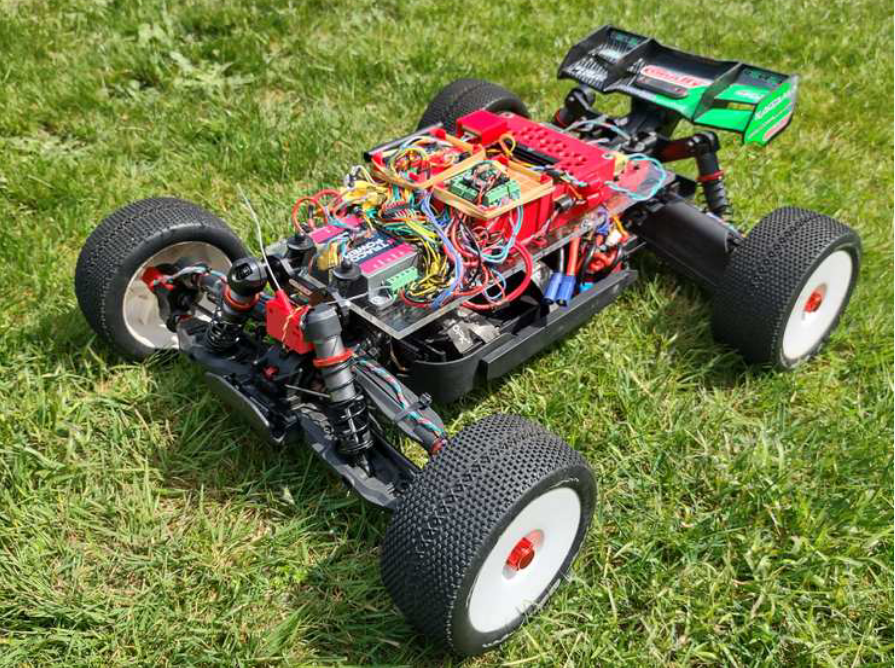
\includegraphics[width=0.5\columnwidth]{images/design/assembly/v1/full_assembly.png}
	\caption{
		TruggySense version 1.
	}
	\label{fig:truggysense_version_1}
\end{figure}

To solve this, most of the components shall be integrated on a custom-made Printed Circuit Board (PCB).
Besides this other expansions this project will aim to include are:
\begin{itemize}
    \item Support for Individual Wheel Drive (IDW).
    \item Expansion possibility to add redundancy.
    \item Integration of ROS2 (Robot Operating System 2).
\end{itemize}

\subsection{Available middleware}
Note that a previous attempt was made to integrate ROS2 on the TruggySense.
Alternatives for this include ArduPilot, PX4, ZeroMQ, and LCM (Lightweight Communications and Marshalling).
Each of them having their advantages and disadvantages:
\begin{itemize}
    \item ArduPilot and PX4 are competitors of each other, both boasting an open-source autopilot firmware.
          These projects were specifically designed for aerial vehicles, later adding support for land vehicles.
          With both ArduPilot and PX4 being designed for autonomy, which isn't suitable for Remote Controlled Vehicles (RCV);
          and having a high reliance on GPS data, which isn't always available in off-road situations.
    \item ROS2 as an open-source middleware framework, working with a Pub-Sub system.
          This project is known to have high latency or bandwidth budgeting, creating the need to alter the software for real-time applications.
    \item ZeroMQ and LCM are open-source messaging libraries, with LCM focussing on real-time data acquisition.
          These projects are both ethernet dependent, ZeroMQ working with TCP and LCM working with UDP.
          With ZeroMQ having no built-in reliability, needing to built your own reconnection and packet loss handling;
          and LCM acting more as a logger than a communication step between the controllers.
\end{itemize}

For this thesis we will continue on the assumption that ROS2 will be implemented, despite its latency issues.

\subsection{Conclusion}
Most of the ground work has been done, yet a small part of the documentation provided is either conflicting, false or non-existing.
Thus this will be an iterative project, first creating a prototype and based on the results and inevitable mishaps a full-fletched PCB will be created.
The goal of this project will be to create second iteration of the TruggySense (TSV2), that will provide a similar performance to the TSV1, but is easier to assemble.

\chapter{Modules and Sensors}       % ---------------------- Modules and Sensors ----------------------
\section{Framework layout} 
The TruggySense makes use of two controllers: A High Level Controller (HLC) and Low Level Controller (LLC).

The LLC will act as a Data Acquisition System (DAQ), control the base components of the RCV and communicate with other components.
The modules used for these purposes are:
\begin{table}[h!]
    \centering
    \begin{tabular}{p{0.3\textwidth}p{0.3\textwidth}p{0.3\textwidth}}
        Sensing: & Actuating: & Communicating: \\
        \begin{itemize}
            \item A motion sensor
            \item A GNSS/GPS
            \item Temperature sensors
            \item Four wheel encoders
        \end{itemize} &
        \begin{itemize}
            \item One to four Electronic Speed Controllers (ESC)
            \item A servo
        \end{itemize} &
        \begin{itemize}
            \item RC control communication
            \item Wireless data logging
        \end{itemize} \\
    \end{tabular}
\end{table}

\begin{figure}[h!]
    \centering
	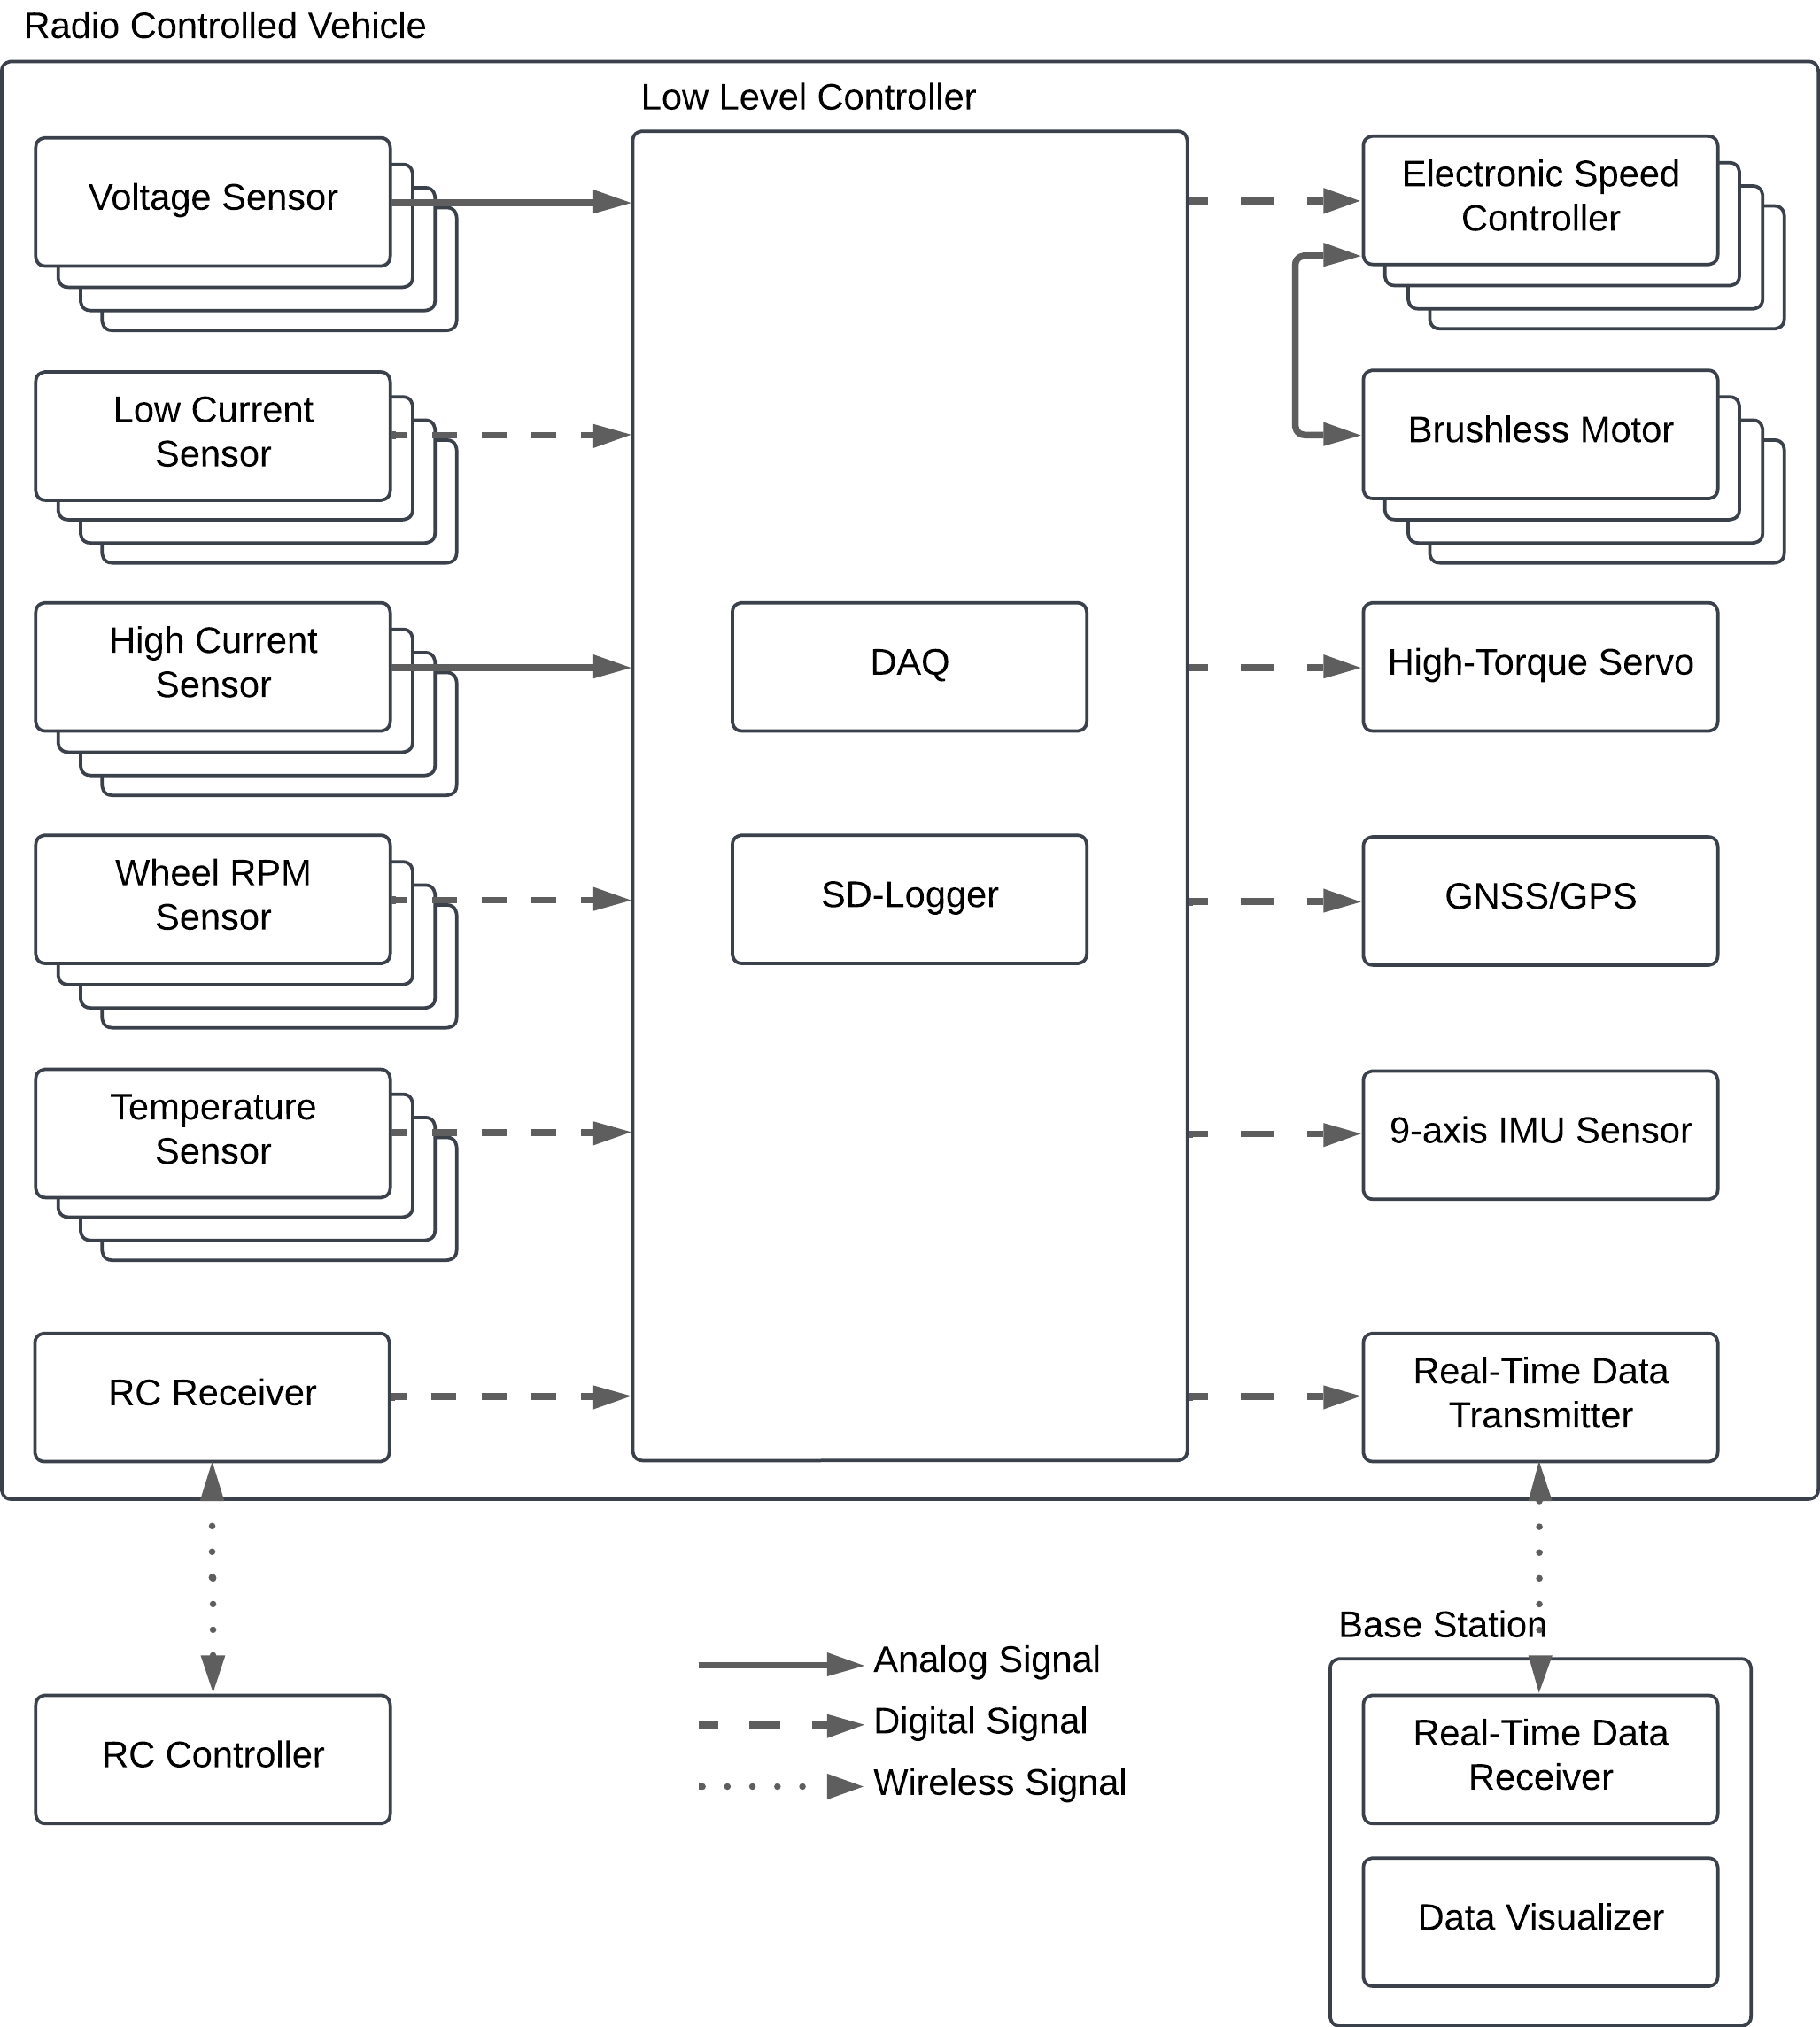
\includegraphics[width=0.5\columnwidth]{images/modules/hardware_architecture.png}
	\caption{
		Hardware architecture of the LLC.
	}
	\label{fig:hardware_architecture}
\end{figure}

The HLC on the other hand will be further expanded on in subsequent stages of this multiple thesis project, 
but it is meant to take the data from the LLC and return instructions to make it a autonomous vehicle.

\section{Low level controller}      % Controllers
\label{sec:LLC}
The module that was both documented and used in the TSV1, was the Teensy 4.1.

As previously discussed ROS2 is intended to be implemented.
This will be done on the HLC, but this is to0 robust for the LLC, thus \href{https://micro.ros.org/docs/overview/hardware/}{Micro-ROS} will be implemented.
This means that we only need to consider Micro-Ros compatible boards fot the LLC.
\HardwareTable
    {low_level_controller}
    {controller/low-level/data.csv}
    {L{4cm} c c r l r}{
        \textbf{Board} & \textbf{RAM} & \textbf{Flash} & 
        \multicolumn{2}{l}{\textbf{Available Pins}} & \textbf{Programmer} \\
    }{
        \href{\BoardURL}{\Component} &
        \RAM & \Flash & \PinHeaderColor{\PinHeaders} &
        \ExtraPins & \ProgrammerColor{\Programmer}
    }

\subsection{Restrictions}
This is an open-source project that any hobbyist should be able to assemble.
For these purposes the following should hold:
\RmLstWS
\begin{itemize}
    \item The LLC needs to be easy to attach and detach from the PCB, meaning that the dev-boards shall be used (unless the chip can easily be soldered on such as with the ESP32).
    \item Programming the software should be simple and available to every user. As such only boards supported by te ArduinoIDE will be used.
    \item The boards should be available on \href{https://www.digikey.be/en}{DigiKey}, \href{https://be.farnell.com/}{Farnell} or \href{https://www.mouser.be/}{Mouser} (and their price should be considered).
    \item The previous model of the TruggySense used the Teensy 4.1 as a LLC. This model contained all needed pins/peripherals to support the connected sensors and actuators, though it did not leave any for future expansions. Thus the LLC should have at least equal or more pins/peripherals available.
\end{itemize}
With these conditions the following boards will not be used:
\RmLstWS
\begin{multicols}{3}
    \begin{itemize}
        \item Renesas EK RA6M5
        \item Espressif ESP32
        \item Arduino Portenta H7
        \item Raspberry Pi Pico RP2040
        \item ROBOTIS OpenCR 1.0
        \item Teensy 3.2
        \item STM32L4 Discovery IoT
        \item Olimex LTD STM32-E407
        \item Arduino Zero
        \item ST NUCLEO-F446ZE
        \item ST NUCLEO-F746ZG
        \item ST NUCLEO-H743ZI
    \end{itemize}
\end{multicols}
\RmLstWS
\RmTabWS
\StockTable
    {low_level_controller}
    {/controller/low-level}
    {28/01/2026}
    {Kiwi}
    {Conrad}
\subsection{Conclusion}
This shows that the only viable option is the Teensy 4.1.
\RmTabWS
\begin{table}[h!]
    \centering
    \caption{Peripherals of Teensy 4.1 dev-board}
    \begin{adjustbox}{max width=\textwidth}
        \begin{tabular}{l c c c c c c c c c c}
            \toprule
                \textbf{Board} & \textbf{GPIO} & \textbf{ADC} &
                \textbf{Timers} & \textbf{PWM} & \textbf{UART} &
                \textbf{SPI} & \textbf{I2C} & \textbf{CAN} & \textbf{SDIO} \\
            \midrule
                \small{Teensy 4.1} & 42 & 
                \small{18$\times$12-bits pins} & \small{4$\times$32-bits} & 
                \small{35 pins} & 8 & 3 & 3 & 2 & 1 \\
            \bottomrule
        \end{tabular}
    \end{adjustbox}
    \label{tab:teensy_peripherals}
\end{table}
\subsection{Power management}
It is recommended to power Teensy 4.1 with a 5V power source, which its on board DC-to-DC converter will convert to 3V3.
A 3V3 could be connected to the 3V3 pin, but is not discouraged.
Its power consumption is estimated to be 100mA (not clear if this is for a 3V3 supply or a 5V supply).
And the maximum allowed power draw for peripherals, that draw power from it, is 250mA at 3V3.

We will assume for now that: the 100 the teensy draws 100mA after the 5V-to-3V3 conversion, and that the peripherals use 200mA of the allowed current.

\hspace{12pt} $P = 3.3V * I_{3V3} = 3.3V * (100mA + 200mA) \approx 1W$

\hspace{12pt} $ I_{5V} = \frac{P}{5V} = \frac{1W}{5V} = 200mA$
\section{High level controller}
\label{sec:HLC}
The module stated in the TSV1 documentation and used was the Nvidia Jetson Nano.
This component cannot be changed as a requirement and thus falls out of this projects scope.
\RmTabWS
\StockTable
    {board_components}
    {/controller/high-level}
    {28/01/2026}
    {Conrad}
    {Antratek}
\subsection{Power management}
The Nvidia Jetson Nano requires a minimum power source of 2A at 5V, but can demand 4A under load.
\newpage

\section{Motion}                    % Sensors
\label{sec:IMU}
In the documentation of the TSV1, on page 10, the following was stated regarding the orientation:

\Quoting{
    The motion of the vehicle will be a vital aspect of the system, since it determines the stability of the vehicle. 
    Therefore, it needs a sensor that can sens movements in the X, Y and Z direction. 
    For this, typically, an Inertial Measurement Unit (IMU) of some degree of freedom is used.
    In our setup, we'll use a 9-Degree-of-Freedom (9DOF) IMU sensor; including angular velocity, acceleration and orientation based on a compass or magnetic sensor.
}

The module that was both documented and used by the TSV1, was the \href{https://www.adafruit.com/product/4754}{BNO085}.
\HardwareTable
    {motion_sensor}
    {sensor/motion/data.csv}
    {L{2cm} L{2.5cm} L{1.5cm} r c l c}{
        \textbf{Sensor} &
        \textbf{Protocol} &
        \textbf{Package} &
        \multicolumn{3}{c}{\textbf{Supply range (V)}} &
        \textbf{Accuracy (DoF)} \\
    }{
        \Component &
        \ProtocolColor{\Protocol} &
        \PackageColor{\Package} &
        \MinSupply & - & \MaxSupply &
        \Accuracy
    }
\RmTabWS
\RmTabWS
\StockTable
    {motion_sensor}
    {/sensor/motion}
    {28/01/2026}
    {Kiwi}
    {Conrad}
\subsection{Conclusion}
Of the two viable options, that being the BNO085 and ICM-20948, the latter is the better choice.
This is due to its lower cost, being more available, smaller board footprint and not conflicting with any other I²C addresses of other modules (see Table~\ref{tab:i2c_address_table}), while still having the same amount of DoF.
\subsection{Power management}
The ICM-20948 requires a average power source of $\sim$5mA at 3V3.
\section{Position}
\label{sec:GPS}
In the documentation of the TSV1, on page 9, the following was stated regarding the positioning:

\Quoting{
    Absolute positioning can be used to estimate the speed of the vehicle. 
    This estimation can be combined with wheel encoders to give a more precise estimation of the actual vehicles speed.
}

The module that was selected in the TSV1, was the \href{https://nl.aliexpress.com/item/1005005211498523.html?spm=a2g0o.productlist.main.67.44796536yggUmW&algo_pvid=d08823a2-dccb-4cfa-b1e2-f92aa56e1174&algo_exp_id=d08823a2-dccb-4cfa-b1e2-f92aa56e1174-33&pdp_npi=4%40dis%21EUR%2114.59%2114.59%21%21%21108.56%21108}{QUESCAN G10A-F30}.
The module that was implemented was the M10FD.
\HardwareTable
    {position_sensor}
    {sensor/position/data.csv}
    {L{2.5cm} L{3.5cm} L{3cm} r c l c}{
        \textbf{Sensor} &
        \textbf{Protocol} &
        \textbf{Package} &
        \multicolumn{3}{c}{\textbf{Supply range (V)}} &
        \textbf{Accuracy (m CEP)} \\
    }{
        \Component &
        \ProtocolColor{\Protocol} &
        \PackageColor{\Package} &
        \MinSupply & - & \MaxSupply &
        \Accuracy
    }
\subsection{Restrictions}
Due to the wide range of modules, filtering will be required, thus the following should hold:
\RmTabWS
\begin{itemize}
    \item Higher accuracy is preferred, thus any module that has a \textgreater2m accuracy will not be considered unless the other options aren't viable.
    \item A smaller footprint is preferred.
    \item Protocols that can be chained together on a single bus, such as I²C and one-wire are preferred.
\end{itemize}
With these conditions the following boards will not be used:
\RmLstWS
\begin{multicols}{3}
    \begin{itemize}
        \item M10FD
        \item L86-M33
        \item PA1616D
        \item CAM-M8
        \item MAX-7
        \item MAX-M8
    \end{itemize}
\end{multicols}
\RmLstWS
\RmTabWS
\StockTable
    {position_sensor}
    {/sensor/position}
    {27/01/2026}
    {Kiwi}
    {Antratek}
\subsection{Conclusion}
Of the listed modules, the NEO-M9N-00B and TESEO-LIV3F are the only viable options.
Of the two viable options, that being the NEO-M9N-00B and TESEO-LIV3F, the latter is the better choice.
This is due to its lower cost, being more available, smaller board footprint and not conflicting with any other I²C addresses of other modules (see Table 2.26), while still having the smallest CEP.
\subsection{Power management}
The TESEO-LIV3F requires a average power source of $\sim$23mA at 3V3.
\section{Temperature}
\label{sec:TMP}
In the documentation of the TSV1, on page 4, the following was stated regarding the temperature sensor:

\Quoting{
    The primary objective of temperature measurements is to monitor the operational condition of all modules in terms of temperature. 
    When measuring temperature, it is possible to identify components nearing failure as well as equipment that may become too hot due to environmental factors or software-induced overheating.\\
    \hfill \break
    Temperature data can be collected at 100Hz. 
    However, in this system, such rapid measurements are unnecessary since we only monitor temperatures outside individual components. 
    Temperature readings must pass through the equipment before any significant increase is detected.
}

The module that was both documented and used by the TSV1, was the \href{https://www.digikey.be/nl/products/detail/analog-devices-inc-maxim-integrated/DS18B20/956983}{DS18B20+}.
Five of these sensors were daisy chained to each other and communicated using the one-wire protocol, with each of them being place against one of the following components:
Brushless motor, Electronic speed controller, Battery pack, Digital servo and High-level controller.
Though it was stated that the sensor for the digital servo was used for the Low-level-controller.
\HardwareTable
    {temperature_sensor}
    {sensor/temperature/data.csv}
    {L{3.5cm} L{3cm} L{1.5cm} r c l r c l c}{
        \textbf{Sensor} &
        \textbf{Protocol} &
        \textbf{Package} &
        \multicolumn{3}{c}{\textbf{Supply range (V)}} &
        \multicolumn{3}{c}{\textbf{Range (°C)}} &
        \textbf{Accuracy (°C)} \\
    }{
        \Component &
        \ProtocolColor{\Protocol} &
        \PackageColor{\Package} &
        \MinSupply & - & \MaxSupply &
        \TempMinTemperatureColor{\MinRange} & - & \MaxRange &
        +/- \Accuracy
    }
\subsection{Restrictions}
A digital sensor was used since sensors will be placed near high current carrier wires that run PWM pulses or the brushless motor, that operate on electromechanical principles.
This could cause significant disturbances to an analogue signal, making it less desirable - though it also could lead to packet loss in case of the digital sensors.

Besides this the pin count on the LLC is limited, making sensors that can be chained to the same bus more favorable.
For this purpose a separate PCB will be designed to make the chaining easier.
This means that the chosen component should be easily soldered using only a solder station.

Thus the following should be held in consideration when choosing a module:
\RmTabWS
\begin{itemize}
    \item Digital protocols are preferred.
    \item Protocols that can be chained together on a single bus, such as I²C and one-wire are preferred.
    \item The temperature sensors need to be mounted on the objects, thus modules that are encased cannot be used.
    \item The chip package should allow manual soldering.
\end{itemize}

With these conditions the following modules will not be used:
\RmTabWS
\begin{multicols}{3}
    \begin{itemize}
        \item DHT11
        \item DHT22
        \item LM35DZ/LM335/LM34
        \item BMP180
        \item TMP36
        \item BME280
    \end{itemize}
\end{multicols}
\RmLstWS
\RmTabWS
\StockTable
    {temperature_sensor}
    {/sensor/temperature}
    {19/01/2026}
    {Kiwi}
    {Otronic}
\subsection{Conclusion}
The LM75 will be chosen due to its low cost and its use of the I²C protocol, without coming into conflict with the addresses of other I²C modules (see Table~\ref{tab:i2c_address_table}).
\subsection{Power management}
There are five LM75 that each require a average power source of 1mA at 3V3 or 5V.
\section{Wheel speed}
\label{sec:ENC}
In the documentation of the TSV1, on page 6, the following was stated regarding the Wheel rotation sensor:

\Quoting{
    The speed of the wheels can be deducted through various approaches such as using a mirror and infra red light (bounce principle), use a white dot (or black) to give contrast and then use a color sensor, a light optic encoder disc or a magnet with a hall effect sensor. 
    This list goes on as many approaches are possible.
    \hfill \break \break
    In this case, the selected approach must endure in harsh conditions where dirt and water can enter the room quite often. 
    The rigidity of the wheel can also not be contaminated. Unbalanced wheels at high RPM’s can cause damage and instability.
    \hfill \break \break
    Therefore, some approaches must be eliminated such as the color sensor, infra-red and mirror - dirt can spoil the party - and optic encoders have an exception. 
    If we had the room to make sure the equipment was well maintained in a dust and water proof encasing, this could work.
    Unfortunate, the space is limited.
}

The module that was both documented and used by the TSV1, was the \href{https://www.mouser.be/ProductDetail/Diodes-Incorporated/AH3323A-P-B?qs=sGAEpiMZZMu5vlrqIFXt5W70N4F8p%252BYG6WxB6YCbiY1gGVb7iWJUbw%3D%3D}{AH3323A-P-B}.
Four of these Uni-Polar sensors were placed on the module, one on each wheel, due to magnetic flux being unaffected by water and dirt.
They provide either a '0' or a '1' if there is any magnetic flux detected, while not needing a reset, as the case with Bi-Polar sensors.

\HardwareTable
    {wheel_speed}
    {sensor/wheel/data.csv}
    {L{4.5cm} L{3cm} L{2.5cm} r c l c c c}{
        \textbf{Sensor} &
        \textbf{Protocol} &
        \textbf{Package} &
        \multicolumn{3}{c}{\textbf{Supply range (V)}} &
        \textbf{Input current (mA)} &
        \textbf{Output current (mA)} &
        \textbf{Accuracy (G)} \\
    }{
        \Component &
        \ProtocolColor{\Protocol} &
        \PackageColor{\Package} &
        \MinSupply & - & \MaxSupply &
        \MaxInA & \MaxOutA &
        \Accuracy
    }

\subsection{Restrictions}
Due to the limited space near the wheels, though hole packages are preferred (such a SIP-3).

Besides the package, the operating voltage should be 3V3, since the Teensy 4.1 isn't protected for 5V signals on its pins.
To convert any 5V signal, a circuit that can convert it to 3V3 would be required, which will only increase the cost and introduce more components that could possibly fail.

Thus the following should be held in consideration when choosing a module:
\RmLstWS
\begin{itemize}
    \item Though hole packages are preferred.
    \item Modules using a 3V3 supply are preferred 
\end{itemize}

With these conditions the following modules will not be used:
\RmLstWS
\begin{multicols}{2}
    \begin{itemize}
        \item TLE4905LE6433
        \item US5881LUA-AAA-000-BU
    \end{itemize}
\end{multicols}
\RmLstWS
\RmTabWS
\StockTable
    {wheel_sensor}
    {/sensor/wheel}
    {28/01/2026}
    {Kiwi}
    {Conrad}
\subsection{Conclusion}
The AH3323A-P-B is still the most accurate and more available than its counterpart.
Thus the AH3323A-P-B will be chosen.
\subsection{Power management}
There are four AH3323A-P-B that each require a average power source of 5mA at 3V3.

\section{Motor}                     % Actuators
\label{sec:MTR}
The module used in the TSV1 was the Corally Kuron 825.
This component cannot be changed as a requirement and thus falls out of this projects scope.

\noindent\textit{No stock of the Corally Kuron 825 was found on available distributors as of 27/01/2026.}

The Corally Kuron 825 requires a maximum power source of 185A between 11V1 and 22V2.
\section{Speed controller}
\label{sec:ESC}
The module used in the TSV1 was the Corally Torox 185.
This component cannot be changed as a requirement and thus falls out of this projects scope.

\noindent\textit{No stock of the Corally Torox 185 was found on available distributors as of 27/01/2026.}

The Corally Torox 185 requires a minimum power source of 100mA at 5V.
\section{Steering servo}
\label{sec:SRV}
The module used in the TSV1 was the DS3225 25KG servo.
This component cannot be changed as a requirement and thus falls out of this projects scope.

\noindent\textit{No stock of the DS3225 was found on available distributors as of 27/01/2026.}

The DS3225 25KG servo requires a minimum power source of 4mA at 5V in idle state, but while rotating it will have a peak current of 1.9A.

\section{RC Control}  % Communication
\label{sec:RCC}
The module stated in the TSV1 documentation and used was the FLySky \href{https://nl.aliexpress.com/item/1005006134316987.html?spm=a2g0o.productlist.main.15.95321a09nW14vW&algo_pvid=9092f028-b0a1-4945-84cc-a7fdfc72d3f0&algo_exp_id=9092f028-b0a1-4945-84cc-a7fdfc72d3f0-7&pdp_npi=4%40dis%21EUR%2141.97%2112.59%21%21%21312.28%2193.68%21%40211b813f17342694926984392e2043%2112000035914037103%21sea%21BE%21723903832%21X&curPageLogUid=dxkHTjTdY4Ll&utparam-url=scene%3Asearch%7Cquery_from%3A}{FS-X6B}, which communicates with a \href{https://nl.aliexpress.com/item/1005006860791905.html?spm=a2g0o.productlist.main.11.95321a09nW14vW&algo_pvid=9092f028-b0a1-4945-84cc-a7fdfc72d3f0&algo_exp_id=9092f028-b0a1-4945-84cc-a7fdfc72d3f0-5&pdp_npi=4%40dis%21EUR%2188.64%2139.89%21%21%21659.52%21296.80%21%40211b813f17342694926984392e2043%2112000044069229511%21sea%21BE%21723903832%21X&curPageLogUid=EwOXjJz6C5DD&utparam-url=scene%3Asearch%7Cquery_from%3A}{FS-I6X} module inside a remote.
This component cannot be changed as a requirement and thus falls out of this projects scope.

\noindent\textit{No stock of the FS-X6B was found on DigiKey, Farnell, Mouser, Kiwi Electronics, Conrad, Antratek or Otronic as of 27/01/2026.}
\subsection{Conclusion}
Since this is an external modules that cannot be integrated on the PCB, it is outside this project's scope to change this module.
Thus we'll continue using the FS-I6X and FS-X6B.
\subsection{Power management}
The FS-X6B requires a power source of 50mA at 5V while transmitting or receiving.
\section{Wireless logging}
\label{sec:LRC}
In the documentation of the TSV1, on page 11-12, the following was stated regarding the long range controller:

\Quoting{
    The communication between vehicle and base station will have a maximum of 500 m, since the FS-X6B transceiver has a range of 500m and 1500m under ideal conditions.
    Thus looking at modules that support longer ranges would hurt nobody.
    \hfill \break \break
    A connection can be setup in two ways.
    Either via a P2P connection with our own modules that connects the RCV and base station, or an access point onto the RCV itself where the user can connect to. 
    With this access point on the vehicle itself, direct communication can be established with any device that supports WiFi.
    This makes connection easier to the vehicle.
}

The module that was both documented and used by the TSV1, was the \href{https://nl.aliexpress.com/item/32783191387.html?spm=a2g0o.productlist.main.1.2bd17c8dH32Wl0&algo_pvid=7b9f4ab4-a0f9-48ab-8d7f-c15a7c529146&algo_exp_id=7b9f4ab4-a0f9-48ab-8d7f-c15a7c529146-0&pdp_npi=4%40dis%21EUR%215.57%213.46%21%21%215.69%213.53%21%402103}{E01-ML01DP5}.
This is a nRF24LO1 module with integrated PA/LNA, making it difficult to find on large distributor marketplaces - such as DigiKey, Farnell and Mouser - since they are mostly non-certified modules.
Thus possible alternatives should be looked towards:
\RmLstWS
\begin{itemize}
    \item nRF24LO1 modules work on 2.4GHz, have added circuits (PA/LNA) and use protocols of smaller size to boost their range.
    This means we could look towards other chips that use the same frequency range, so we have support of the WiFi infrastructure.
    Chips like these include the other nRF24LO1 modules and modules from the nRF52 with an external PA/PLA or optimized antenna.
    \item Sub-1GHz modules have a longer range and better penetration than 2.4GHz modules.
    Chips like these include the nRF905, TI CC11 and TI CC13 modules.
\end{itemize}

Wi-Fi/Bluetooth modules, such as the ESP32 or ATWINC1500, cannot be used with the same modifications as the nRF52.
The 2.4GHz radio is too tightly coupled to the Wi-Fi/Bluetooth protocols, that making changes is impossible.
This lowers the range of the modules drastically to but a few hundred meters at best.

Modules with a standard sub-1GHz protocol, such as LoRa, have the range, but might not have the needed infrastructure to support it (LoRa needs gateways) and have a limit on how many messages can be send per hour/day.
\begin{table}[h!]
    \centering
    \caption{Long range alternatives table}
    \begin{adjustbox}{max width=\textwidth}
        \begin{tabular}{l c c c c}
            \toprule
                \textbf{Module} & \textbf{Frequency} & \textbf{PA/LNA} & \textbf{Protocol} & \textbf{Estimated range} \\
            \midrule
                FLySky X6B  & 2.4 GHz & Moderate   & AFHDS 2A & $\sim$200-500m \\
                E01-ML01DP5 & 2.4 GHz & Integrated & ESB      & $\sim$800m-1.5 km \\
            \midrule
                CC11     & 433/868/915 MHz & Integrated & Software defined & \CommunicationRangeColor{$\sim$1-2km} \\
                CC13     & 433/868/915 MHz & Integrated & Software defined & \CommunicationRangeColor{$\sim$1-2km} \\
                CC25     & 2.4 GHz         & None       & Software defined & \CommunicationRangeColor{$\sim$50-100m} \\
                CC25     & 2.4 GHz         & External   & Software defined & \CommunicationRangeColor{$\sim$500-800m} \\
                ESP32    & 2.4 GHz         & None       & BLE/Wi-Fi        & \CommunicationRangeColor{$\sim$50-200m} \\
                nRF24    & 2.4 GHz         & None       & ESB              & \CommunicationRangeColor{$\sim$50-100m} \\
                nRF24L01 & 2.4 GHz         & Integrated & ESB              & \CommunicationRangeColor{$\sim$500m-1km} \\
                nRF52    & 2.4 GHz         & None       & BLE/Zigbee       & \CommunicationRangeColor{$\sim$50-100m} \\
                nRF52    & 2.4 GHz         & External   & BLE/Wi-Fi        & \CommunicationRangeColor{$\sim$500m-1km} \\
                nRF905   & 433/868/915 MHz & Moderate   & Hardware defined & \CommunicationRangeColor{$\sim$500m-1km} \\
            \bottomrule
        \end{tabular}
    \end{adjustbox}
    \label{tab:long_range_alternatives}
\end{table}
\RmTabWS
\RmTabWS
\HardwareTable
    {long_range_communication}
    {communication/nrf/data.csv}
    {L{3cm} L{3.5cm} L{3cm} r c l c c c}{
        \textbf{Sensor} & \textbf{Protocol} & \textbf{Package} & 
        \multicolumn{3}{c}{\textbf{Supply range (V)}} &
        \textbf{Frequency} & \textbf{Antenna} & \textbf{Range}\\
    }{
        \Component & \ProtocolColor{\Protocol} & 
        \PackageColor{\Package} &
        \MinSupply & - & \MaxSupply &
        \Frequency & \Antenna & \CommunicationRangeColor{\Range}
    }

\subsection{Restrictions}
For the module to be useful it first needs to have a longer range than the RC communication module (500m), and should even exceed this.
\StockTable
    {long_range_communication}
    {/communication/nrf}
    {01/02/2026}
    {Conrad}
    {Otronic}
\subsection{Conclusion}
The two viable options are the BDE-RFM208P and WIRL-WMB8 Metis-e.
Upon further research the \href{https://www.bdecomm.com/uploads/2021913/20210913173678807880.pdf}{BDE-RFM208P} needs a \href{https://www.ti.com/tool/LAUNCHXL-CC1352P#order-start-development}{TI CC1352P development kid} which would cost 50\$.
This isn't a software that is free to use software and thus falls out of the constraints of this project.
As for the \href{https://www.we-online.com/en/components/products/METIS-E}{WIRL-WMB8 Metis-e} can only be programmed using a software that is only available for Windows, and thus falls out of the constraints of this project.
\newpage
Since both the viable options are not available, we will return to the NRF24L01.
Note that these boards are only useful if a PA/PLA is present.
\RmFigWS
\begin{figure}[h!]
    \caption{Difference between PA/LNA and none ~\cite{Dejan2022}.}
    \centering
    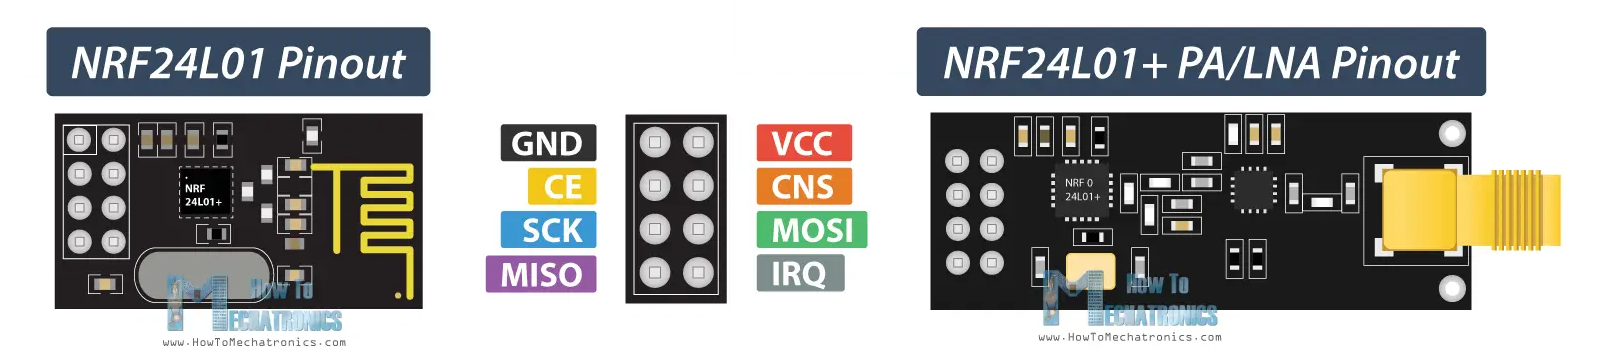
\includegraphics[width=0.69\textwidth, center]{images/modules/pa_pla_difference.png}
    \label{fig:pa_pla_difference}
\end{figure}
\RmFigWS
\subsection{Power management}
The NRF24L01 requires a power source of 13mA at 3V3 while transmitting or receiving.

\section{Supply}                    % Supply
The supply used in the TSV1 was the \href{https://www.amazon.com.be/Gens-ace-Batterie-connecteur-Connection/dp/B09YXRSTMT?source=ps-sl-shoppingads-lpcontext&psc=1}{Gens ace 4S Lipo Battery 5000mAh 14.8V 50C 4S Bashing RC Battery}.
When fully charged this module will provide a 16.8V supply that will diminish to 12.8V when discharging.
\RmTabWS
\begin{table}[h!]
    \centering
    \caption{Power draw estimation}
    \begin{adjustbox}{max width=\textwidth}
        \begin{tabular}{l r c c c c}
            \toprule
                \textbf{Module} & \textbf{Function} & \textbf{Quantity} & 
                \textbf{3V3 current (mA)} & \textbf{5V current (mA)} & 
                \textbf{5V load current (mA)} \\
            \midrule
                Teensy 4.1          & \hyperref[sec:LLC]{LLC}           & 1 &    & 200  & 200  \\
                NVIDIA JETSON NANO  & \hyperref[sec:HLC]{HLC}           & 1 &    & 2000 & 4000 \\
                ICM-20948           & \hyperref[sec:IMU]{Motion}        & 1 & 5  &      & \\
                TESEO-LIV3F         & \hyperref[sec:GPS]{Position}      & 1 & 23 &      & \\
                LM75                & \hyperref[sec:TMP]{Temperature}   & 5 & 1  &      & \\
                AH3323A-P-B         & \hyperref[sec:ENC]{Wheel speed}   & 4 & 5  &      & \\
                Torox 185           & \hyperref[sec:ESC]{Wheel Speed}   & 1 &    & 100  & 100  \\
                DS3225              & \hyperref[sec:SRV]{Servo}         & 1 &    & 4    & 1900 \\
                FS-X6B              & \hyperref[sec:RCC]{RC control}    & 1 &    & 50   & 50   \\
                nRF24L01            & \hyperref[sec:LRC]{Long range}    & 1 & 13 &      & \\
                ACS758              & \hyperref[sec:AMP]{Current}       & 1 & 4  &      & \\
                INA219              & \hyperref[sec:AMP]{Current}       & 4 & 1  &      & \\
            \midrule
                Total               &               &   & 74 & 2154 & 6250 \\
            \bottomrule
        \end{tabular}
    \end{adjustbox}
    \label{tab:power_draw_estimation}
\end{table}
\section{DC/DC converter}
\label{sec:power_conversion}
The modules stated in the TSV1 documentation were the \href{https://nl.aliexpress.com/item/1005006376332910.html?spm=a2g0o.productlist.main.1.69bf8p638p63NM&algo_pvid=98bb040f-81ae-4e6f-a6b8-e5eca0064604&algo_exp_id=98bb040f-81ae-4e6f-a6b8-e5eca0064604-0&pdp_npi=4%40dis%21EUR%214.81%211.39%21%21%2135.80%2110.38%21}{Mini560PRO-3.3V} and \href{https://nl.aliexpress.com/item/1005006376332910.html?spm=a2g0o.productlist.main.1.69bf8p638p63NM&algo_pvid=98bb040f-81ae-4e6f-a6b8-e5eca0064604&algo_exp_id=98bb040f-81ae-4e6f-a6b8-e5eca0064604-0&pdp_npi=4%40dis%21EUR%214.81%211.39%21%21%2135.80%2110.38%21}{Mini560PRO-5V}.
The modules that were used were the LA3484A and the TMDC 20-2411.

The entire system connected to the LLC will have a current draw of around 2.5A.
To make sure this current can be provided, a module that can provide at least 1.5 times that amount (3.75A) will be used.
The TMDC 20-2411 Isolated Module can provide a current of 4A, demands an 9-36V input - between which the battery's voltage swings remain - and can output a steady 5.1V.
This module might be replaced by its 40W (TMDC 40-2411) or 60W counterpart (TMDC 60-2411), depending on the current draw.

A benefit to this module is that the source and sink voltages are separated at both the positive and negative terminals.
That way the battery and motor can be connected to a PCB that is separated, both physically and with its ground plane, from the LLC PCB.
This will give the following benefits:
\RmLstWS
\begin{itemize}
    \item The logic board will be separated from the motor's return current, leading to less noise.
    \item Any drops in voltage or current spikes won't effect the 5V rail, leading to a stiffer supply.
\end{itemize}
\HardwareTable
    {DC/DC_converter}
    {power/converter/data.csv}
    {L{3cm} L{3cm} r c l r c l c}{
        \textbf{Sensor} & \textbf{Package} &
        \multicolumn{3}{c}{\textbf{Input voltage (V)}} &
        \multicolumn{3}{c}{\textbf{Output voltage (V)}} &
        \textbf{Max current (A)} \\
    }{
        \Component & \PackageColor{\Package} &
        \AboveValueColor{4.8}{\MinInV}  & - & \BelowValueColor{5}{\MaxInV} &
        \AboveValueColor{3.3}{\MinOutV} & - & \BelowValueColor{3.3}{\MaxOutV} &
        \BelowValueColor{0.2}{\MaxAmp}
    }
\subsection{Restrictions}
With these conditions the following boards will not be used:
\RmLstWS
\begin{multicols}{4}
    \begin{itemize}
        \item AMS1117-3.3
        \item AMS1117-5.0
        \item D45V5F5
        \item JW5068A
        \item LA3484A
        \item LM7805
        \item Mini560PRO-3.3V
        \item Mini560PRO-5V
        \item S13V20F5
        \item S7V8F5
        \item S9V11F5
        \item XL1509-5.0
        \item XL4015
        \item XL4016
    \end{itemize}
\end{multicols}
\RmLstWS
\RmTabWS
\StockTable
    {power_supply}
    {/power/converter}
    {02/02/2026}
    {Conrad}
    {Otronic}
\subsection{Conclusion}
There are four viable options: LM2596, MP2338GTL-Z, TPS62A0X, TPS631000DRLR.
Of these modules the LM2596 is the most expensive, both the board and its parts are readily available.
Besides that, all needed components of the board are easy to solder.
Thus the LM2596 will be used as an alternative to the integrated circuit provided on the LLC.
\section{Ampere meter}
\label{sec:AMP}
In the documentation of the TSV1, on page 8, the following was stated regarding the ampere meter sensor:

\Quoting{
    The current consumption of modules can give an indication on faulty hardware or even faulty software.
    It is more a monitoring value. Nevertheless, this ”monitoring” is vital in order to not overrun our hardware.
    \hfill \break \break
    For this, two methods of determining current consumption can be utilized:
    Shunt resistors, which measure the differential voltage across a resistor in series; 
    and Hall-effect sensors, which measure the current based on the magnetic field they create while passing through a conductor.
    \hfill \break \break
    We could divide high and low currents, where we measure the former with the hall effect sensing methodology and the latter with a shunt resistor.
}

The modules that wer both documented and used by the TSV1 were the \href{https://www.digikey.com/en/products/detail/allegro-microsystems/ACS758ECB-200B-PFF-T/2042748}{ACS758ECB-200B-PFF-T}, for high current, and \href{https://www.adafruit.com/product/1164}{INA169}, for low current.
\HardwareTable
    {high_ampere_meter}
    {sensor/current/data_high.csv}
    {L{1.5cm} L{4.5cm} L{3cm} r c l r c l r c l l}{
        \textbf{Sensor} &
        \textbf{Communication protocol} &
        \textbf{Package} &
        \multicolumn{3}{c}{\textbf{Supply range (V)}} &
        \multicolumn{3}{c}{\textbf{Readable voltage (V)}} &
        \multicolumn{3}{c}{\textbf{Readable current (A)}} &
        \textbf{Accuracy (mV/A)} \\
    }{
        \Component & \ProtocolColor{\Protocol} & 
        \PackageColor{\Package} &
        \MinSupply & - & \MaxSupply &
        \MinReadV & - & \MaxReadV &
        \MinReadA & - & \MaxReadA &
        \Accuracy   
    }
\RmTabWS
\RmTabWS
\HardwareTable
    {low_ampere_meter}
    {sensor/current/data_low.csv}
    {L{1.5cm} L{4.5cm} L{3cm} r c l r c l r c l}{
        \textbf{Sensor} &
        \textbf{Communication protocol} &
        \textbf{Package} &
        \multicolumn{3}{c}{\textbf{Supply range (V)}} &
        \multicolumn{3}{c}{\textbf{Readable voltage (V)}} &
        \multicolumn{3}{c}{\textbf{Readable current (A)}} \\
    }{
        \Component & \ProtocolColor{\Protocol} & 
        \PackageColor{\Package} &
        \MinSupply & - & \MaxSupply &
        \MinReadV & - & \MaxReadV &
        \MinReadA & - & \MaxReadA
    }

\subsection{Restrictions}
The motor has a power requirement of of 181A at a voltage between 11.1V and 22.2V, meaning the high current sensor needs to abide by this.

The remaining modules all work with either a 3V3 or 5V supply, but their current draw needs to be accounted for, since the INA-modules have a maximum current based on the Shunt-resistor.

With these conditions the following boards will not be used:
\RmLstWS
\begin{multicols}{2}
    \begin{itemize}
        \item ACS712
        \item ACS725
    \end{itemize}
\end{multicols}
\RmLstWS
\RmTabWS
\StockTable
    {amp_meter}
    {/sensor/current}
    {28/01/2026}
    {Kiwi}
    {Conrad}
\subsection{Conclusion}
For the high current application between the battery and the motor, the ACS758ECB-200U-PFF-T will be used as before.

For the low current applications between battery and computing board, the INA219 wil be used due to it supporting I²C without coming into conflict with the other I²C modules (see Table~\ref{tab:i2c_address_table}).
This will open three analogue ports up for later expansions.
Though slight modifications need to be made to these modules since their standard 100m\si{\ohm} (resulting in a maximum allowed current of 3.2A) will damage the INA-modules when the system is under load.

Instead of using four INA-modules, four will be implemented:
\RmLstWS
\begin{itemize}
    \item One for the overall current draw place at the input of the TMDC 20-2411.
    \item One for the HLC, which have a current draw between 2-4A.
    \item One for the RC-actuators, servo and motor control, which have a current draw between 100mA-2A.
    \item One for the LLC and its peripherals.
\end{itemize}

The INA219 can measure the voltage across a Shunt resistor, up to 320mV.
Thus the following rule should be followed:

\hspace{12pt} $I * R_{Shunt} < 320mV \Leftrightarrow R_{Shunt} < \frac{320mV}{I}$

\begin{table}[h!]
    \centering
    \caption{Current sensor modification}
    \begin{adjustbox}{max width=\textwidth}
        \begin{tabular}{l c rl rl rcl rcl}
            \toprule
                \textbf{Measuring} &
                \textbf{$I$} &
                \multicolumn{2}{c}{\textbf{$R_{Shunt}$}} &
                \multicolumn{2}{c}{\textbf{$V_{drop}$}} &
                \multicolumn{3}{c}{\textbf{Supply range (V)}} &
                \multicolumn{3}{c}{\textbf{Allowed supply (V)}} \\
            \midrule
                Overall logic current & 6.25A & $\frac{320mV}{6.25A} = 51.2m\Omega$ & $\Rightarrow R_{Shunt} = 50m\Omega$  & $ 6.25A * 50m\Omega $  & $= 312.5mV $ & 12.8 & - & 16.8 & 9    & - & 36 \\
                HLC                   & 4A    & $\frac{320mV}{4A} = 80m\Omega$      & $\Rightarrow R_{Shunt} = 50m\Omega$  & $ 4A * 50m\Omega $     & $= 200mV $   & 5.1  & - & 5.1  & 4.75 & - & 5.25 \\
                RC-actuators          & 2A    & $\frac{320mV}{2A} = 160m\Omega$     & $\Rightarrow R_{Shunt} = 100m\Omega$ & $ 2A * 100m\Omega $    & $= 200mV $   & 5.1  & - & 5.1  & 4.8  & - & 6.8 \\
                LLC + peripherals     & 200mA & $\frac{320mV}{200mA} = 1.6\Omega$   & $\Rightarrow R_{Shunt} = 100m\Omega$ & $ 200mA * 100m\Omega $ & $= 20mV $    & 5.1  & - & 5.1  & 4.8  & - & 5.5 \\
            \bottomrule
        \end{tabular}
    \end{adjustbox}
    \label{tab:current_sensor_modification_table}
\end{table}
This table shows that only two of the four INA-modules need their Shunt resistors replaced, and that by cutting their resistance in halve, they won't cause a voltage drop that will lead to the modules not functioning anymore.
\subsection{Power management}
There are four INA219 that each require a minimum power source of 1mA at 3V3, and one ACS758 that requires a minimum power source of 4mA at 3V3.
\section{Volt meter}
In the documentation of the TSV1, on page 7, the following was stated regarding the volt meter sensor:

\Quoting{
    Voltage monitoring is essential at several points in the system: 
    the total voltage of the battery pack, the individual cell voltages, and the voltages of the various power supplies.
    \hfill \break \break
    One approach is to measure these voltages directly using the Analogue to Digital Converter (ADC) on the Microcontroller Unit (MCU). 
    While this is a valid and straightforward method, analog signals are often susceptible to noise, which can distort the readings. 
    To mitigate this, additional hardware is needed to filter out unwanted noise.
    This can be achieved using analog components such as low-pass filters or inductive coils, or digitally using techniques like a moving average filter of size N.
    \hfill \break \break \newpage
    The chosen Teensy 4.1 MCU features 18 analog input pins, distributed across two ADC units. 
    For voltage measurements alone, a minimum of seven pins is needed: two for power sources, one for total battery voltage, and four for individual cell voltages. 
    While the ADC supports up to 12-bit resolution, it is generally recommended to use 10-bit resolution for stability and speed accordingly to the community. 
    This provides a usable range of \(2^{10}=1024\) levels, resulting in a voltage resolution of approximately \(\frac{3.3V}{1024bit}\simeq 3.22\frac{mV}{bit}\), assuming a reference voltage of 3.3V .
    Since many of the system voltages exceed 3.3V, voltage dividers must be used to scale the signals down to within the ADC’s readable range.
    After each voltage divider, a buffer stage (typically an op-amp configured as a voltage follower) should be added.
    This ensures the ADC sees a low-impedance source, while also preserving the integrity of the voltage divider's output.
}

The module that was selected in the TSV1, was the \href{https://www.adafruit.com/product/1083}{ADS1015}, but it also stated that it wouldn't use these and utilize the LLCs on-board ADCs.

\HardwareTable
    {volt_meter}
    {sensor/voltage/data.csv}
    {L{2cm} L{5cm} L{5cm} r c l r c l c}{
        \textbf{Sensor} &
        \textbf{Communication protocol} &
        \textbf{Package} &
        \multicolumn{3}{c}{\textbf{Supply range (V)}} &
        \multicolumn{3}{c}{\textbf{Output voltage (V)}} &
        \textbf{Accuracy} \\
    }{
        \Component &
        \ProtocolColor{\Protocol} &
        \PackageColor{\Package} &
        \MinSupply & - & \MaxSupply &
        \MinRange & - & \MaxRange &
        \Accuracy-bit
    }

\subsection{Restrictions}
Both of these sensors only have 4 I²C addresses, ranging from 0x48 to 0x4B.
Not only can they not support the 7 applications that need an ADC, but they also overlap with the other I²C modules (see Table~\ref{tab:i2c_address_table}).
\subsection{Conclusion}
Seven of the analogue pins of the LLC will be used in tandem with a buffer circuit that will convert any 5V signal to a safe 3V3.

\section{I²C address table overview}
\begin{table}[h!]
    \centering
    \caption{I²C address table}
    \begin{adjustbox}{max width=\textwidth}
        \begin{tabular}{l r c c c c c c c c c c c c c c c c c c c c}
            \toprule
                \textbf{Module} & \textbf{Function} & \textbf{\#} &
                \multicolumn{19}{c}{\textbf{Addresses}}\\
            \midrule
                BNO085      & Motion      & 0 &&&&&&&&&& 0x48 & 0x49 &&&&&&&&  \\
                ICM-20948   & Motion      & 1 &&&&&&&&&&&&&&&&&& 0x68 & \IICUses{0x69} \\
                NEO-M9N-00B & Position    & 0 &&&& 0x42 &&&&&&&&&&&&&&&  \\
                TESEO-LIV3F & Position    & 1 & \IICUses{0x3A} &&&&&&&&&&&&&&&&&  \\
                LM75        & Temperature & 5 &&&&&&&&&& 0x48 & 0x49 & 0x4A & \IICUses{0x4B} & \IICUses{0x4C} & \IICUses{0x4D} & \IICUses{0x4E} & \IICUses{0x4F} && \\
                INA219      & Current     & 4 && \IICUses{0x40} & \IICUses{0x41} & \IICForb{0x42} & \IICForb{0x43} & \IICUses{0x44} & \IICUses{0x45} & \IICForb{0x46} & \IICForb{0x47} & \IICForb{0x48} & \IICForb{0x49} & \IICForb{0x4A} & \IICForb{0x4B} & \IICForb{0x4C} & \IICForb{0x4D} & \IICForb{0x4E} & \IICForb{0x4F} && \\
            \bottomrule
        \end{tabular}
    \end{adjustbox}
    \label{tab:i2c_address_table}
\end{table}

Note that the INA219 can have 16 I²C addresses, but these depend on with which lines the A0 and A1 pins are connected (GND, VS, SDA or SCL).
Since the dev-board only allows for connection to GND and VS, the address range drops to 4 addresses.

\chapter{Module functionality}      % ---------------------- Module functionality ----------------------
\section{Protocols}
\subsection{ADC}
The LLC (Teensy 4.1) contains 14 ADC inputs.
These inputs are rated to allow voltages of up to 3.6V, but can only measure up to 3.3V.
To still be able to read the voltages of other rails, voltage deviders can be used.

\vspace{-18pt}
\begin{align}
    U_{out}                                   & = \frac{R_{2}}{R_{1} + R_{2}} \cdot U_{in} \\
    U_{out} \cdot (R_{1} + R_{2})             & = R_{2} \cdot U_{in} \\
    U_{out} \cdot R_{1} + U_{out} \cdot R_{2} & = R_{2} \cdot U_{in} \\
    U_{out} \cdot R_{1}                       & = R_{2} \cdot U_{in} - R_{2} \cdot U_{out} \\
    U_{out} \cdot R_{1}                       & = R_{2} \cdot (U_{in} - U_{out}) \\
    R_{2}                                     & = R_{1} \cdot \frac{U_{out}}{(U_{in} - U_{out})}
\end{align}
\vspace{-6pt}

With $R_{1}$ bridging between $U_{in}$ and $U_{out}$, and $R_{2}$ bridging between $U_{out}$ and GND.

It is best to use a 10kΩ - 100kΩ resitor value for $R_{1}$, to minimize the leak current, and to round the calculated value of $R_{2}$ to its closest E12 counterpart.

The LLC (Teensy 4.1) make use of 12-bit counters, resulting in $2^{n} = 2^{12} = 4096$ measurable voltage levels.
For this project this is set to 10-bit counters, resulting in 1024 measurable voltage level, meaning that the rounding error of the ADC can be found as follows:

\vspace{-18pt}
\begin{align}
    U_{per level} & = \frac{U_{cc}}{N} \\
                  & = \frac{3.3V}{1024} \\
                  & = 3.22mV
\end{align}
\vspace{-6pt}

\RmFigWS
\begin{figure}[h!]
    \centering
    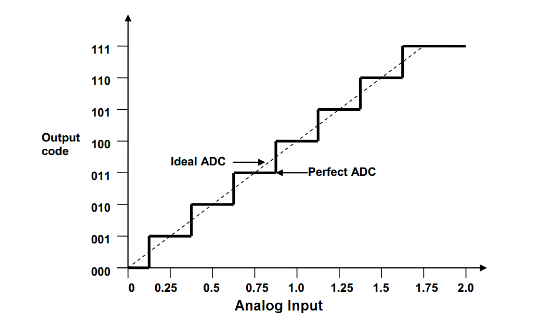
\includegraphics[width=0.5\textwidth, center]{images/explenations/adc.png}
    \caption{ADC voltage level conversion~\cite{Pefhany2017}.}
\end{figure}
\RmFigWS

This means that if we want to measure the 5V rail (ussually this is at 5.1V) dropping to 4.85V, that we would need a voltage devider of:

\vspace{-18pt}
\begin{align}
    R_{2} & = 10k\Omega \cdot \frac{3.3V}{(5.1V - 3.3V)} \\
          & = 18.33k\Omega \\
          & \approx 18k\Omega
\end{align}
\vspace{-6pt}

Our measured value at 4.85V then becomes:

\vspace{-18pt}
\begin{align}
    U_{out} & = \frac{18k\Omega}{10k\Omega + 18k\Omega} \cdot 4.85V \\
            & = 3.11786V \\
    U_{ADC} & = 3.11786V - (3.11786V \% 3.22mV) \\
            & = 3.11786V - 0.9mV\\
            & = 3.11696V
\end{align}
\vspace{-6pt}

If our software reverses the down-conversion with the measure data, we get a 0.0024V difference:

\vspace{-18pt}
\begin{align}
    U_{in} & = \frac{R_{1} + R_{2}}{R_{2}} \cdot U_{out} \\
           & = \frac{10k\Omega + 18k\Omega}{18k\Omega} \cdot 3.11696V \\
           & = 4.8486V
\end{align}
\vspace{-6pt}
\subsection{PWM}
The LLC (Teensy 4.1) contains 28 PWM outputs.
These outputs can generate a PWM at 3.3V.

The two most important aspects of a PWM signal are: its period (the dureation of the complete pulse, and the inverse of the frequency), and duty-cycle (a percentile of the period, in which the pulse is active).

\RmFigWS
\begin{figure}[h!]
    \centering
    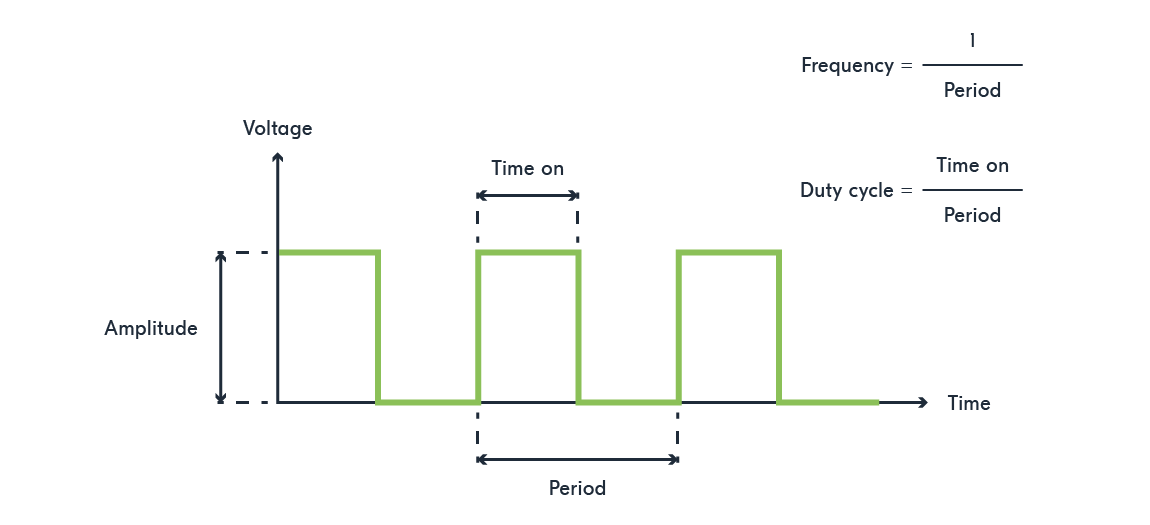
\includegraphics[width=0.60\textwidth, center]{images/explenations/pwm.png}
    \caption{PWM structure~\cite{Dev2026}.}
\end{figure}
\RmFigWS

\clearpage
\subsection{I2C}
The LLC (Teensy 4.1) contains 3 seperate I²C busses.
Each I²C bus allows one master node and multiple slave nodes to be attach simultaniously.
In our implementation, the LLC will always act as the I²C master.
I²C makes use of two lines: The SDA line (act as the data line) and the SCL line (provide a clock signal so that the modules are in sync).

\RmFigWS
\begin{figure}[h!]
    \centering
    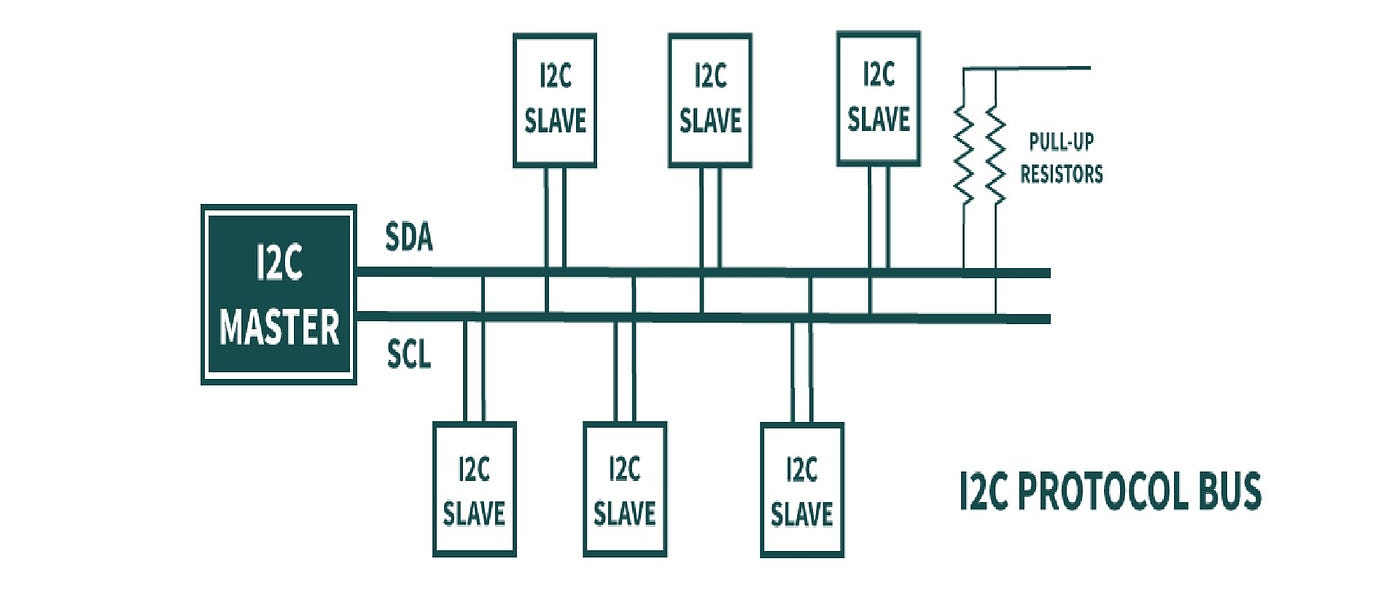
\includegraphics[width=0.60\textwidth, center]{images/explenations/i2c_setup.png}
    \caption{I²C bus layout~\cite{Ouiyzme2023}.}
\end{figure}
\RmFigWS

The master node will send out:
\RmLstWS
\begin{itemize}
    \item A start bit to initialize the conversation with the slave nodes.
    \item An address frame. All slaves will see this address, but only the slave to which the address belongs will answer.
    \item A bit that indicates if the master nodes wants to send or receive data.
    \item The acknowledgement of the slave.
    \item The data frames (one byte) the were either send or requested by the master node.
    \item Acknowledgement from the recipient.
    \item A stop bit to end the connection.
\end{itemize}
\RmLstWS

\RmFigWS
\begin{figure}[h!]
    \centering
    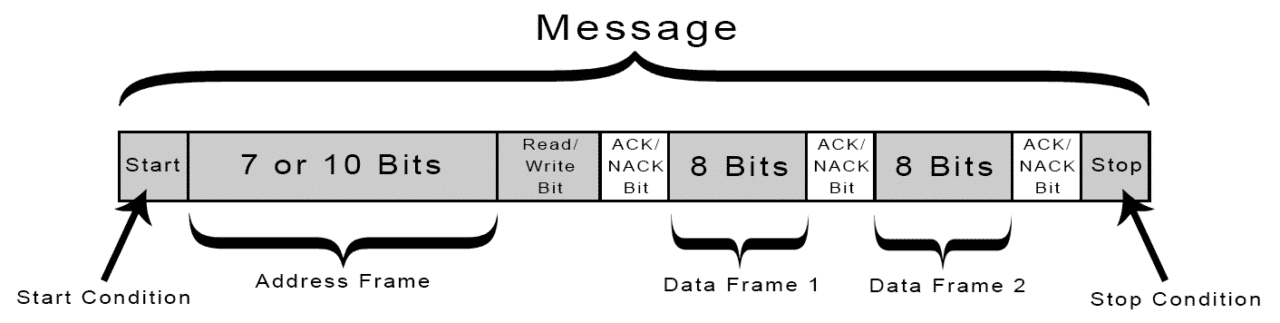
\includegraphics[width=0.60\textwidth, center]{images/explenations/i2c_signal.png}
    \caption{I²C message layout~\cite{Circuit2016}.}
\end{figure}
\RmFigWS

The standart speed supported by the LLC for I²C is 100kbps (kilo bits per second).
Using different modes this could be increased to 400kbps or 1Mbps.
\subsection{SPI}
The LLC (Teensy 4.1) contains 2 seperate SPI busses.
Each SPI bus allows for one master node and multiple slave nodes.
In our implementation, the LLC will always act as the SPI master.
SPI makes use of four lines:
\RmLstWS
\begin{itemize}
    \item The CS/SS (chip/slave select) line, will indicate with which slave the master will communicate.
          The master will need to provide a CS line for each slave on the same bus.
          It indicates when it wants to communicate with a specific slave, by setting the CS line LOW.
    \item The SCLK/SCK (clock) line, which acts as a reference on which the data is send and to keep all modules in sync.
    \item The MOSI (master out, slave in) line, is used when the master wants to send data to the slave.
    \item The MISO (master in, slave out) line, is used when the master wants to receive data from the slave.
\end{itemize}
\RmLstWS

\clearpage
\ImageComparison
    {SPI layout}
    {spi_layout}
    {{explenations/spi_setup.png}/{Bus layout~\cite{Microcontroller2026}}
    /{explenations/spi_signal.png}/{Signal example~\cite{Rohde2023}}}
\RmFigWS

The LLC has a reliable clock speed of 40MHz.
This means that it has a throughput of 40Mbps.
\subsection{UART}
The LLC (Teensy 4.1) contains 8 seperate UART busses.
Each UART bus allows for two nodes.
UART makes use of two lines: The TX (transmit) line and the RX (receive) line.
Note that the TX pin of node one needs to be connected to the RX pin of node two, and vice versa.

\RmFigWS
\ImageComparison
    {UART layout}
    {uart_layout}
    {{explenations/uart_setup.png}/{Bus layout~\cite{Kelvin2022}}
    /{explenations/uart_signal.png}/{Signal example~\cite{Kelvin2022}}}
\RmFigWS

Most UART modules use the default settings. These are a baud rate of 9600 --corresponding to a transmission speed of 9600 bits per second (bps)-- with an 8N1 configuration.
UART always starts with one start-bit, and the 8N1 notation indicates the following: '8' indicates eight data-bits are send per frame, 'N' indicates that no parity-bit is used, and '1' indicates one stop-bit is used.
This means that every byte needs 10 bits to be send, resulting in a transmission speed of 960 bytes per second (Bps) or a byte period of $\sim$1.04ms.
Both the baud rate and configuration can be changed, but in our implementation only the baud rate will be adjusted to 115200.
\section{Modules}
\subsection{LED}
An led will be added to the logic board, to indicate if the system has initialized correctly.

\RmFigWS
\begin{figure}[h!]
    \centering
    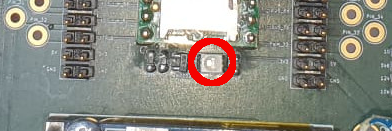
\includegraphics[width=0.60\textwidth, center]{images/explenations/led.png}
    \caption{Indicator led.}
\end{figure}
\RmFigWS

\clearpage
When this led is:
\RmLstWS
\begin{itemize}
    \item On, it indicates that the initialization is in progress.
    \item Off, it indicates that the initialization has failed.
    \item Toggles, it indicates that the initialization was succesfull and that the schedular is activated.
\end{itemize}
\RmLstWS
\subsection{Motor}
When using the Torox 185, make sure to set the system correctly.

\RmFigWS
\begin{figure}[h!]
    \centering
    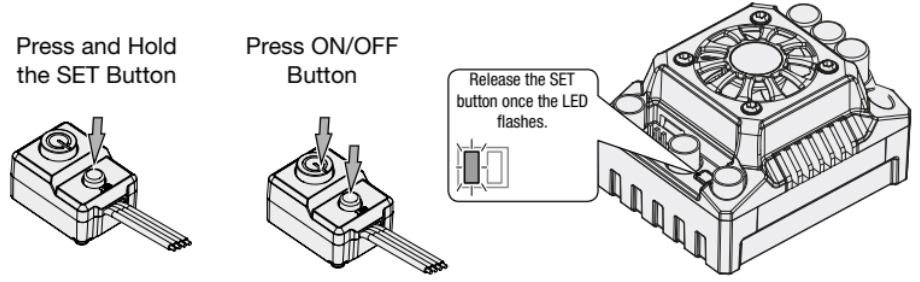
\includegraphics[width=0.60\textwidth, center]{images/explenations/esc.png}
    \caption{ESC module~\cite{Corally2026}.}
\end{figure}
\RmFigWS

First of all, we need to enable reverse driving.
This is done by pressing and holding both the ON/OFF and SET buttons, until the Green led toggles.
You are now in running mode.
In this mode the system will portray the configuration every 10 seconds using a blinking red led and beep.
The configuration is as follows:
\RmLstWS
\begin{itemize}
    \item 1 blink \rightarrow~Forward with brake.
    \item 2 blink \rightarrow~Forward / Reverse with brake.
\end{itemize}
\RmLstWS
Turn the system off to save the configuration.

To calibrate the system, first press the ON/OFF button.
A green led will blink 4 times, 1 for each LiPo cell it detects\footnote{It will just measure the voltage. If the voltage is above 14.8V, then you should get this effect.}.
Afterwards the red led will toggle constantly until the neutral position is administered.
This is done by providing a 50Hz PWM (20ms period), with an active time of 1500µs (1.5ms).
Once calibrated the led will stop toggling, and any PWM signal with a higher duty-cycle than the neutral position will activate the motor.
\subsection{FlySky}
% Add FlySky connect:   https://www.youtube.com/watch?v=q80QijmQzOI
% Remote Control:       https://youtu.be/JZQoHmLqZYg?si=V70LEDVfeEnfySdj
The first thing to do when using FlySky modules is to bind them.
To start this, on the reciever board, press the "Bind" Button (the button at the edge of the board), while powering on the module.
The led should be blinking quite fast now.
Now on the transitter module, press the "Bind" Button (the button next to the bottom left corner of the screen) and power it on.
The red led on the receiver should now be solid, this means that the modules are bound.
\href{https://www.youtube.com/watch?v=q80QijmQzOI}{Follow \textbf{this video} if needed.}

Now to set the auxilary ports.
The transmitter supports 14 channels that send a value between 1000 and 2000.
The first four channels are locked to the horizontal and vertical movement of the joysticks.
The other channels can be configured as followed:
\RmLstWS
\begin{itemize}
    \item Turn on the transmitter.
    \item Press and hold the "OK" button.
          This should open the menu.
    \item Choose "System setup" by pressing the "OK" button.
    \item Then use the "UP" and "DOWN" buttons to go to the bottom of the list and select "Aux. switches".
    \item Turn on the swithces you want to use.
    \item Press and hold "CANCEL" to save.
    \item Turn off the transmitter.
\end{itemize}

\begin{itemize}
    \item Turn on the transmitter back on.
    \item Press and hold the "OK" button, opening the menu.
    \item Choose "Functions setup".
    \item Scroll down to "Aux. channels".
    \item Use the "UP" and "DOWN" buttons to bind a switch to a channel.
    \item Press and hold "CANCEL" to save.
    \item Turn off the transmitter.
\end{itemize}
\RmLstWS
\href{https://www.youtube.com/watch?v=JZQoHmLqZYg}{Follow \textbf{this video} if needed.}

Note that for this project channel 5 is connected to SWA.
This switch acts as the deadswitch of the entire system.

\RmFigWS
\ImageComparison
    {FlySky system}
    {flysky_system}
    {{explenations/fs_x6b.png}/{Transmitter~\cite{FlySky2016}}
    /{explenations/fs_i6x.png}/{Receiver~\cite{Pete2026}}}
\RmFigWS
\subsection{GPS}
The GPS makes use of a u-blox module.
From this we can conlcude that the system uses the default configuration (baud rate 9600 and config 8N1), and that this can be changed using the \href{https://www.u-blox.com/en/product/u-center}{\textbf{u-center application}}.
The problem is that this application only runs on Windows, and that not all modules allow configuration changes to be saved to the flash.

Still the communication speed of the module needs to be altered since the default settings provide a byte period of $\sim$1.04ms, and the schedular of the system uses synchronous interrupts that repeat every 1ms.
If the communication speed was set to 115200, the byte period would become $\sim$86.81µs, making the schedular less of a problem.
This will be performed during the initialization of the system (before the schedular is activated).
By sending the right byte array the configuration can be altered (this will reset at power down).

The following configuration changes are sent at startup:
\RmLstWS
\begin{itemize}
    \item Disable the GLL, GSA, GSV, and VTG data.
          This data isn't used and therefore can be turned off.
    \item Set the update rate to 10Hz.
          This will provide us with more data.
    \item Set the baud rate to 115200.
\end{itemize}
\RmLstWS
\clearpage
\subsection{Wheel encoders}
The wheel encoders work using asynchronous interrupts.
When these hall-effect sensors detect a magnet they pull the signal line down.
A counter then keeps track of how many magnets have passed, and using the following formulas, the wheel can be determined:
\begin{align}
    t_\Delta &= \frac{t_1 - t_0}{1000} \\
    f_p      &= \frac{1}{t_\Delta} \\
    f_w      &= \frac{f_p \cdot n_p}{N_\text{mag}} \\
    \omega_w &= f_w \cdot 60 \\
    t_\Delta &= \frac{t_1 - t_0}{1000} \\
    f_w      &= \frac{1}{t_\Delta} \cdot \frac{n_p}{N_\text{mag}}\\
    \omega_w &= f_w \cdot 60
\end{align}
With $t\Delta$ representing the periode of the pulses (in seconds), $f_p$ the frequency of the pulse (in Herz), 
$X$ the number of magnets installed on the encoder ring, $\omega_w$ the rotational speed (in revolutions per second),
$d$ the diameter (in meters), $v$ the velocity (kilometer per hour), and $n_p$ denoting the number of pulses detected~\cite{Elsermans2025}.

\RmFigWS
\begin{figure}[h!]
    \centering
    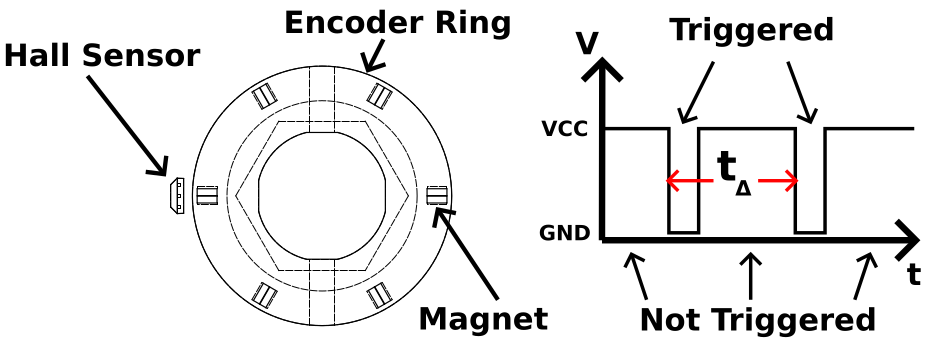
\includegraphics[width=0.40\textwidth, center]{images/explenations/encoder.png}
    \caption{Encoder ring structure~\cite{Elsermans2025}.}
\end{figure}
\RmFigWS
\subsection{IMU}
The IMU works over I²C and collects 9-DoF information, inlcuding 3-DoF accelerometer data, 3-DoF gyroscope data, and 3-DoF magnetometer data.
Each of the 3-DoF data sets are reperesented by a x, y, and z number.
These 9-DoF values can be converted to quaternion\footnote{A quaternion is another way of representing 3D rotation.} using a Mahony filter.
These are the steps:
\begin{enumerate}
    \item Timing & Sample Frequency:
        \begin{align}
            t_\Delta & = \frac{t_1 - t_0}{10^6} \\
            f_s      & = \frac{1}{t_\Delta}
        \end{align}
        With $f_s$ the sample frequency (in Herz).
    \item Normalise accelerometer data:
        \begin{align}
            a_{norm} & = \frac{1}{\sqrt{a_x^2 + a_y^2 + a_z^2}} \\
            a_x      & = a_x \cdot a_{norm} \\
            a_y      & = a_y \cdot a_{norm} \\
            a_z      & = a_z \cdot a_{norm}
        \end{align}
        With $a$ representing the normalized acceleration vector.
    \item Normalise magnetometer data:
        \begin{align}
            m_{norm} & = \frac{1}{\sqrt{m_x^2 + m_y^2 + m_z^2}}\\
            m_x      & = m_x \cdot m_{norm} \\
            m_y      & = m_y \cdot m_{norm} \\
            m_z      & = m_z \cdot m_{norm}
        \end{align}
        With $m$ representing the normalized magnetometer vector.
    \item Reference the data to the direction of Earth's magnetic field:
        \begin{align}
            h_x &= 2\!\left[m_x\!\left(\tfrac{1}{2} - q_2^2 - q_3^2\right) + m_y(q_1 q_2 - q_0 q_3) + m_z(q_1 q_3 + q_0 q_2)\right] \\
            h_y &= 2\!\left[m_x(q_1 q_2 + q_0 q_3) + m_y\!\left(\tfrac{1}{2} - q_1^2 - q_3^2\right) + m_z(q_2 q_3 - q_0 q_1)\right] \\
            b_x &= \sqrt{h_x^2 + h_y^2} \\
            b_z &= 2\!\left[m_x(q_1 q_3 - q_0 q_2) + m_y(q_2 q_3 + q_0 q_1) + m_z\!\left(\tfrac{1}{2} - q_1^2 - q_2^2\right)\right]
        \end{align}
        With $h$ representing the magnetic field vector, and $b$ Earth's magnetic field vector.
    \item Estimated direction of gravity and magnetic field
        \begin{align}
            \tfrac{1}{2}v_x &= q_1 q_3 - q_0 q_2 \\
            \tfrac{1}{2}v_y &= q_0 q_1 + q_2 q_3 \\
            \tfrac{1}{2}v_z &= q_0^2 - \tfrac{1}{2} + q_3^2 \\[6pt]
            \tfrac{1}{2}w_x &= b_x\!\left(\tfrac{1}{2} - q_2^2 - q_3^2\right) + b_z(q_1 q_3 - q_0 q_2) \\
            \tfrac{1}{2}w_y &= b_x(q_1 q_2 - q_0 q_3) + b_z(q_0 q_1 + q_2 q_3) \\
            \tfrac{1}{2}w_z &= b_x(q_1 q_3 + q_0 q_2) + b_z\!\left(\tfrac{1}{2} - q_1^2 - q_2^2\right)
        \end{align}
        With $v$ representing the gravity vector, and $w$ estimated magnetic field vector.
    \item Find the error (Cross Product):
        \begin{align}
            \tfrac{1}{2}e_x &= (a_y \cdot \tfrac{1}{2}v_z - a_z \cdot \tfrac{1}{2}v_y) + (m_y \cdot \tfrac{1}{2}w_z - m_z \cdot \tfrac{1}{2}w_y) \\
            \tfrac{1}{2}e_y &= (a_z \cdot \tfrac{1}{2}v_x - a_x \cdot \tfrac{1}{2}v_z) + (m_z \cdot \tfrac{1}{2}w_x - m_x \cdot \tfrac{1}{2}w_z) \\
            \tfrac{1}{2}e_z &= (a_x \cdot \tfrac{1}{2}v_y - a_y \cdot \tfrac{1}{2}v_x) + (m_x \cdot \tfrac{1}{2}w_y - m_y \cdot \tfrac{1}{2}w_x)
        \end{align}
        With $e$ representing the error vector.
    \item Apply integral feedback:
        \begin{align}
            I_x &\mathrel{+}= \frac{2K_i \cdot \tfrac{1}{2}e_x}{f_s} \\
            g_x &\mathrel{+}= I_x \\
            I_y &\mathrel{+}= \frac{2K_i \cdot \tfrac{1}{2}e_y}{f_s} \\
            g_y &\mathrel{+}= I_y \\
            I_z &\mathrel{+}= \frac{2K_i \cdot \tfrac{1}{2}e_z}{f_s} \\
            g_z &\mathrel{+}= I_z
        \end{align}
        With $I$ representing the integral feedback accumulation, and $g$ representing the gyroscope vector.
    \item Apply proportional feedback: 
        \begin{align}
            g_x &\mathrel{+}= 2K_p \cdot \tfrac{1}{2}e_x \\
            g_y &\mathrel{+}= 2K_p \cdot \tfrac{1}{2}e_y \\
            g_z &\mathrel{+}= 2K_p \cdot \tfrac{1}{2}e_z
        \end{align}
    \item Add the new values to the quaternions:
        \begin{align}
            q_0 &\mathrel{+}= \left(-q_1 g_x - q_2 g_y - q_3 g_z\right)\frac{\Delta t}{2} \\
            q_1 &\mathrel{+}= \left(\phantom{-}q_0 g_x + q_2 g_z - q_3 g_y\right)\frac{\Delta t}{2} \\
            q_2 &\mathrel{+}= \left(\phantom{-}q_0 g_y - q_1 g_z + q_3 g_x\right)\frac{\Delta t}{2} \\
            q_3 &\mathrel{+}= \left(\phantom{-}q_0 g_z + q_1 g_y - q_2 g_x\right)\frac{\Delta t}{2}
        \end{align}
\end{enumerate}
With the constatnts $\Delta t = \frac{1}{f_s}, \qquad 2K_p = 2.0, \qquad 2K_i = 0.005$.

These quaternions can then be converted to Euler/orientation angles, using the following code:
\begin{enumerate}
    \item Quaternion Normalisation
        \begin{align}
            r         &= \frac{1}{\sqrt{q_0^2 + q_1^2 + q_2^2 + q_3^2}} \\
            \hat{q}_i &= q_i \cdot r \quad \text{for } i \in \{0, 1, 2, 3\}
        \end{align}
    \item Euler Angles from Quaternion
        \begin{align}
            \phi   &= \frac{360}{2\pi}\arctan\!\left(\frac{2(q_0 q_1 + q_2 q_3)}{1 - 2(q_1^2 + q_2^2)}\right) \\[6pt]
            \theta &= \frac{360}{2\pi}\arcsin\!\left(2(q_0 q_2 - q_3 q_1)\right) \\[6pt]
            \psi   &= \frac{360}{2\pi}\arctan\!\left(\frac{2(q_0 q_3 + q_1 q_2)}{1 - 2(q_2^2 + q_3^2)}\right)
        \end{align}
\end{enumerate}
With the constatnts $\frac{360}{2\pi} = \frac{180}{\pi} \approx 57.296 \quad \text{(radians to degrees)}$.

The orientation angles of the modules are always noted on top off them.
Make sure that they are in the correct orientation compared to the chassis.

\RmFigWS
\begin{figure}[h!]
    \centering
    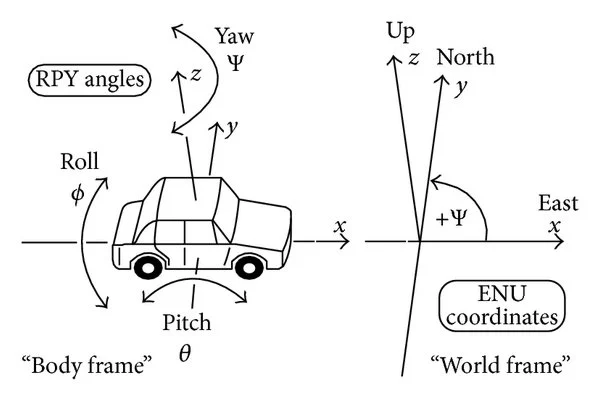
\includegraphics[width=0.378\textwidth, center]{images/explenations/orientation_angles.png}
    \caption{Orientation angles~\cite{Yi2015}.}
\end{figure}
\clearpage
\subsection{SD-card}
The LLC provides SD-card intregation, thus we can implement persistent data.
The default way to store the gathered data is in a .bin file.
To study the data, support for both .csv and .json files has been added.
The .json files are needed by the matlab scripts that generate the graphs later used.

Make sure that the SD-cards are formated in NTFS.
\subsection{nRF24L01}
This module makes use of the SPI protocol.
The thing to look out for is that it has both a CS and CE pin.
Neither of these pins need to be connected to the CS pin of the LLC, they only have to be connected to a PWM pin.
Note that in the code these pins have to be altered to match the hardware.

This project only got the receiver module to work, while it was attached to an Arduino UNO.
Here is the sketch that was used:
\begin{lstlisting}[style=platformio]
/*
* Arduino Wireless Communication Tutorial
*       Example 1 - Receiver Code
*                
* by Dejan Nedelkovski, www.HowToMechatronics.com
* 
* Library: TMRh20/RF24, https://github.com/tmrh20/RF24/
*/

#include <SPI.h>
#include <nRF24L01.h>
#include <RF24.h>

RF24 radio(7,8); // CE, CSN 7, 8

const byte address[6] = "00001";

void setup() {
  Serial.begin(115200);
  pinMode(LED_BUILTIN, OUTPUT);
  digitalWrite(LED_BUILTIN, LOW);
  
  while (!Serial) { }
  Serial.println("Receiver on");
  digitalWrite(LED_BUILTIN, HIGH);
  
  if (!radio.begin()) {
    Serial.println("radio.begin() FAILED — SPI not working");
    while(1);
  }
  if (!radio.isChipConnected()) {
    Serial.println("nRF24L01 not detected! Check wiring/power.");
    // while (1);  // halt
  } else
    Serial.println("Chip connected OK");
  radio.openReadingPipe(0, address);
  radio.setPALevel(RF24_PA_MIN);
  radio.setChannel(76);
  //radio.setAutoAck(false);
  //Serial.println("=== Radio Config ===");
  //radio.printDetails();   // dumps all registers
  //Serial.println("=== Listening ===");
  radio.startListening();
}

void loop() {
  // Serial.println("Listening...");  // temporary debug line
  /*if (radio.available()) {
    char text[32] = "";
    radio.read(&text, sizeof(text));
    Serial.println(text);
  }*/
  if (radio.available()) {
    uint8_t chunk[32] = {0};
    radio.read(&chunk, sizeof(chunk));
    
    uint8_t chunkIndex = chunk[0];
    if (chunkIndex == 0) Serial.println();
    Serial.print("Read chunk ");
    Serial.print(chunkIndex);
    Serial.print(":\t");
    
    for (int j = 0; j < 32; j++) {
      if (chunk[j] < 0x10) Serial.print("0");
      Serial.print(chunk[j], HEX);
      Serial.print(" ");
    }
    
    Serial.println();
  }
}
\end{lstlisting}

\chapter{Prototype Design}          % ---------------------- Prototype design ----------------------
\section{Logical design}
\RmFigWS
\begin{figure}[h!]
    \caption{TruggySense logic interaction between modules}
    \centering
    
\includegraphics[width=1\textwidth, center]{images/design/lucidchart/prototype/logic_layout.png}
\end{figure}
\newpage
\section{Power design}
\RmFigWS
\begin{figure}[h!]
    \caption{TruggySense power interaction between modules}
    \centering
    
\includegraphics[width=1\textwidth, center]{images/design/lucidchart/prototype/power_layout.png}
\end{figure}
\RmFigWS
\section{KiCAD}
KiCAD 9.0 was used to design the PCBs.
The guide below will show how to install KiCAD and showcase the base functionalities.
\subsection{Guide}
\label{sec:kicad_guide}
\subsubsection{Install KiCAD}
The installation for Windows can be found using \href{https://www.kicad.org/download/windows/}{this link}.

The installation for Linux (Debian and Ubuntu) can be done using the following commands:
\begin{lstlisting}[style=cmd]
# Install KiCad:
    sudo apt update && sudo apt install -t kicad kicad-symbols kicad-footprints kicad-packages3d

# Verify success:
    kicad --version
\end{lstlisting}
\RmLstWS\RmTabWS
\subsubsection{Add component library}
% Logic for the row count
\newcount\TotalRows                 % Create a CSV row variable
\TotalRows=0                        % Set it to 0
\csvreader[head to column names]{./databases/design/download.csv}{}{
    \global\advance\TotalRows by 1  % Increment for every CSV row
}
%\the\TotalRows                      % Show the row count
% Half row rounded up
\newcount\HalfRow                   % Create a half row variable
\HalfRow=\numexpr\TotalRows/2\relax
%\the\HalfRow                        % Show the row count
% Next row
\newcount\NextRow
\NextRow=\numexpr\HalfRow+1\relax
%\the\NextRow                        % Show the row count

\Needspace{10\baselineskip}
\begin{table}[h!]
    \centering
    \caption{Component usage overview}
    \begin{minipage}[t]{0.47\textwidth}
        \centering
        \begin{tabular}{p{0.47\textwidth} p{0.47\textwidth}}
            \toprule
                \textbf{Component} & \textbf{Used in} \\
            \midrule
                \csvreader[
                    head to column names,
                    late after line=\\,
                    range=0-\HalfRow,
                ]{./databases/design/download.csv}{}{
                    \href{\CompURL}{\Component} & \UsedIn
                }
            \bottomrule
        \end{tabular}
    \end{minipage}
    \hfill
    \begin{minipage}[t]{0.47\textwidth}
        \centering
        \begin{tabular}{p{0.47\textwidth} p{0.47\textwidth}}
            \toprule
                \textbf{Component} & \textbf{Used in} \\
            \midrule
                \csvreader[
                    head to column names,
                    late after line=\\,
                    range=\NextRow-\TotalRows,
                ]{./databases/design/download.csv}{}{
                    \href{\CompURL}{\Component} & \UsedIn
                }
            \bottomrule
        \end{tabular}
    \end{minipage}
\end{table}
\RmTabWS
\begin{enumerate}[label*=\arabic*., nosep]
    \item From the main project window.
    \item Click the "preferences" tab.
    \item Click "Manage Symbols Library".
    \begin{enumerate}[label*=\arabic*., nosep]
        \item Click "Add existing library to the table" (folder-icon on the bottom left).
        \item Go to the \verb|.kicad_sym| file and select it.
        \item Click "OK".
    \end{enumerate}
    \item Click "Manage Footprint Library".
    \begin{enumerate}[label*=\arabic*., nosep]
        \item Click "Add existing library to the table" (folder-icon on the bottom left).
        \item Go to the \verb|.kicad_sym| file and select its folder.
        \item Click "OK".
    \end{enumerate}
    \item Open the schematic and press 'A'.
    \item Choose the symbol and dropt it into the schematic.
    \item Double click on the component.
    \item Change the footprint.
\end{enumerate}

Add shortcuts to the right files to make your life easier.
For Debian users this can be done as follows:
\begin{lstlisting}[style=cmd]
# Connect the repo symbol directory to that of the installation:
    ln -s ~/<path_to_repo>/TruggySense/cad/KiCAD/library ~/.local/share/kicad/9.0/symbols/

# Connect the repo footprint directory to that of the installation:
    ln -s ~/<path_to_repo>/TruggySense/cad/KiCAD/library ~/.local/share/kicad/9.0/footprints/
\end{lstlisting}
\subsubsection{Schematic hot keys}
\RmLstWS
\begin{multicols}{3}
    \begin{itemize}[label={}]
        \IconItem{kicad/icons/schematic/annotate}{Annotate schematic}
        \IconItem{kicad/icons/schematic/rules_check}{Electrical rules check}
        \IconItem{kicad/icons/schematic/assign}{Assign footprint}
        \IconItem{kicad/icons/schematic/bom}{Bill of materials}
        \IconItem{kicad/icons/schematic/pcb}{PCB editor}
        \IconItem{kicad/icons/schematic/symbol}{A - Add symbol}
        \IconItem{kicad/icons/schematic/power}{P - Add power symbol}
        \IconItem{kicad/icons/schematic/wire}{W - Wire routing}
        \IconItem{kicad/icons/schematic/float}{Q - Add unconnected pins}
        \IconItem{kicad/icons/schematic/global_label}{L - Add global label}
        \IconItem{kicad/icons/schematic/sheet_label}{H - Add hierarchical label}
        \IconItem{kicad/icons/schematic/sheet}{S - Draw hierarchical sheet}
    \end{itemize}
\end{multicols}
\RmLstWS\RmLstWS\RmLstWS
\subsubsection{Link footprint to symbol}
\RmLstWS
\begin{enumerate}[label*=\arabic*., nosep]
    \item Open the "Symbol Editor".
    \item Open the desired symbol.
    \item Click "File" \textgreater~"Symbol properties".
    \item Assign a default footprint.
\end{enumerate}
\RmLstWS\RmLstWS
\subsubsection{Make a component inactive}
\RmLstWS
Inactive component for non repetition of component reference. Double click component and check:
\RmLstWS
\begin{itemize}
    \item Exclude from simulation
    \item Exclude from bill of materials
    \item Exclude from board
    \item Do not populate
\end{itemize}
\RmLstWS\RmLstWS
\subsubsection{PCB hot keys}
\RmLstWS
\begin{multicols}{3}
    \begin{itemize}[label={}]
        \IconItem{kicad/icons/board/setup}{Board setup}
        \IconItem{kicad/icons/board/3D}{ALT+3 - 3D viewer}
        \IconItem{kicad/icons/board/import_parts}{F8 - Update from schematic}
        \IconItem{kicad/icons/board/rules_check}{Design rules checker}
        \IconItem{kicad/icons/board/schematic}{Scheamtic editor}
        \IconItem{kicad/icons/board/wire}{X - Route track}
        \IconItem{kicad/icons/board/via}{Ctrl+Shift+X - Place via}
        \IconItem{kicad/icons/board/filled_zone}{Ctrl+Shift+Z - Filled zone}
        \IconItem{kicad/icons/board/rules_zone}{Ctrl+Shift+K - Rules area}
        \IconItem{kicad/icons/board/line}{Ctrl+Shift+L - Draw line}
        \IconItem{kicad/icons/board/arc}{Ctrl+Shift+A - Draw arc}
        \IconItem{kicad/icons/board/text}{Ctrl+Shift+T - Draw text}
        \item V - Switch between top and bottom copper layer
        \item + - Switch to the next copper layer
        \item - - Switch to the previous copper layer
    \end{itemize}
\end{multicols}
\RmLstWS\RmLstWS\RmLstWS
\subsubsection{Update PCB from schematic}\RmLstWS
To add new components, check both "Replace footprints..." and "Update footprint".

To delete old components, check "Delete footprints...".

To reattach footprints to their symbol, check \textbf{only} "Re-link footprints...".
\RmLstWS
\subsubsection{Change board layer amount}
\RmLstWS
Got to: PCB design \textgreater~Board setup \textgreater~Board stackup \textgreater~Physical stackup \textgreater~Copper Layers = 4
\RmLstWS
\subsection{File structure}
\label{sec:kicad_file_structure}
As mentioned before (see section \hyperref[sec:power_conversion]{2.13 DC/DC converter}), 
PCB that contains the connection to the battery and motor will be split from the PCB containing all the logic components.
This can be seen by the files:
\RmLstWS
\begin{enumerate}[label*=\arabic*., nosep]
    \item Logic board
    \item Power board
\end{enumerate}

Of these two, the logic board makes multiple uses of the IO-protection circuits:
\RmLstWS
\begin{enumerate}[label*=\arabic*., nosep]
    \item Buffer
    \item Input
    \item Output
\end{enumerate}
\RmLstWS
By referring to these files when making a new sheet, any change made to one of the protection circuits, will be made to all of the same type.
Note that the low-pass filter/voltage divider sketch also belongs to this category.

The layout files, are footprints of modules that could not be found online. These include:
\RmLstWS
\begin{enumerate}[label*=\arabic*., nosep]
    \item nRF24L01
    \item PIM448
\end{enumerate}
\RmLstWS
Note that these files will be deleted in the next version because the PIM448 will be added to the library of footprints, 
and the current nRF24L01 footprint (in use) accommodates for both the nRF24 modules with a built in antenna and external antenna.
This is because while designing the part and logic PCB, I knew that the "L01" specified that the modules had a longer range,
but what I didn't know was that this referred to only the modules with an external antenna (as seen in \hyperref[fig:pa_pla_difference]{Figure 2.1}).

The remaining sketches are self made designs. These include both recreations and original designs:
\RmLstWS
\begin{enumerate}[label*=\arabic*., nosep]
    \item INA219 recreation
    \item LM2596 recreation
    \item Position sensor
    \item Temperature sensor
\end{enumerate}
\RmLstWS
The recreations give a wider choice of options, since the modules aren't always available, 
but components often are (as can be seen in both \hyperref[tab:power_supply_available_stock]{Table 2.18} and \hyperref[tab:amp_meter_available_stock]{Table 2.19}).
\newpage
\subsection{Schematic}
\subsubsection{Logic board}
\RmFigWS
These are the schematics of the logic board:
\begin{figure}[h!]
    \caption{TruggySense logic board electrical schematics}
    \centering
    
\includegraphics[width=1\textwidth, center]{images/design/kicad/schematic/v2/logic.png}
\end{figure}

\RmFigWS
Note that the "ADC"-schematic is the same as the LP-filter/voltage divider schematic.
\ImageComparison
    {TruggySense logic board communication circuits electrical schematics}
    {logic_coms_schematics}
    {{design/kicad/schematic/v2/logic_i2c.png}/{I²C circuit design (TruggySense v2)}
    /{design/kicad/schematic/v2/logic_uart.png}/{UART circuit design (TruggySense v2)},
    {design/kicad/schematic/v2/logic_spi.png}/{SPI circuit design (TruggySense v2)}
    /{design/kicad/schematic/v2/logic_pwm.png}/{PWM circuit design (TruggySense v2)},
    {design/kicad/schematic/v2/logic_input.png}/{Various communications design (TruggySense v2)}
    /{design/kicad/schematic/v2/logic_pins.png}/{Pin header design (TruggySense v2)}}
\RmFigWS
Note that both types of \href{https://electronics.stackexchange.com/a/186182}{UART voltage conversion} have been used in this project.
Bidirectional for the IBUS line, and unidirectional for the USB line.
\newpage
\subsubsection{Power board}
\RmFigWS
This is the schematics of the power board:
\begin{figure}[h!]
    \caption{TruggySense power board electrical schematics}
    \centering
    
\includegraphics[width=0.32\textwidth, center]{images/design/kicad/schematic/v2/power.png}
\end{figure}
\RmFigWS
\subsubsection{Sensor boards}
\RmLstWS
This is the schematics of the sensor boards:
\ImageComparison
    {TruggySense external sensor boards electrical schematics}
    {sensor_schematics}
    {{design/kicad/schematic/v2/sensor_position.png}/{Position sensor design (TruggySense v2)}
    /{design/kicad/schematic/v2/sensor_temperature.png}/{Temperature sensor design (TruggySense v2)}}
\RmFigWS
\newpage
\subsubsection{IO-protection}
\RmLstWS
This is the schematics of the IO-protection circuits:
\ImageComparison
    {TruggySense IO-protection electrical schematics}
    {io_protection_schematics}
    {{design/kicad/schematic/v2/io_protection_input.png}/{Input design (TruggySense v2)}
    /{design/kicad/schematic/v2/io_protection_buffer.png}/{Buffer design (TruggySense v2)},
    {design/kicad/schematic/v2/io_protection_output.png}/{Output design (TruggySense v2)}
    /{design/kicad/schematic/v2/lpf_voltage_divider.png}/{LP-filter/voltage divider design (TruggySense v2)}}
\RmFigWS
\subsubsection{Recreations}
\RmLstWS
This is the schematics of the recreated board layout:
\ImageComparison
    {Recreated electrical schematics}
    {recreation_schematics}
    {{design/kicad/schematic/v2/ina219.png}/{INA219 design (TruggySense v2)}
    /{design/kicad/schematic/v2/lm2596.png}/{LM2596 design (TruggySense v2)}}
\newpage
\subsubsection{Fixes}
The Teensy 4.1 only functions on 3V3 logic, with a maximum current output of 4mA.
Thus 5V modules such as the FLySky-X6B, DS3225, or any motor would be impossible without conversion to 5V.
Besides that the if a modules, such as the FLySky-X6B, would communicate back to the LLC, than its ports would be damaged.
And finally, any module connected to an input pin of the LLC can have surge currents or interference from surrounding modules, thus filters and IO protection will be required.

\NoteCreate{overvoltage}{Overvoltage is the raising of voltage beyond the design limit of the circuit.~\cite{Wikipedia2026_Overvoltage}}
\NoteCreate{transient}{A transient event involves abrupt changes in voltage and/or current.~\cite{Keysight2025}}
\NoteCreate{ESD}{Electrostatic discharge (ESD) is a sudden and momentary release of the stored static electricity between two differently-charged objects.~\cite{Wikipedia2026_ESD} This can drastically increase the voltage on a trace for a short time.}
\paragraph{Input protection}
\ComponentTable{explenations/io_protection_input.csv}
The zener-diode will enter its breakdown quickly, but turn on slowly (µs); while TVC-diode will breakdown slowly and turn on fast (ns).
When these two are placed together in this circuit and ESD occurs, then the zener-diode conducts and heats up, while the TVS cannot fully engage due to the zener-diode.
That is why the zener-diode needs to be removed.
It is meant to keep an unchanging line stable, but this input is continuously changing, making it a hindrance instead of a help.
\ImageComparison
    {TruggySense input protection electrical schematic}
    {io_protection_input_schematic}
    {{design/kicad/schematic/v1/io_protection_input.png}/{Old input design (TruggySense v1)}
    /{design/kicad/schematic/v2/io_protection_input.png}/{New input design (TruggySense v2)}}
\paragraph{Protection buffer}
\ComponentTable{explenations/io_protection_buffer.csv}
The source of the buffer is set to 5V.
This means that the buffer 5V signals into the LLC (which can only handle 3V3 signals).

Besides that an input resistor will be added with similar functions to the output resistors.
Decoupling the capacitance of the input and protecting against ESD.
\ImageComparison
    {TruggySense protection buffer electrical schematic}
    {io_protection_buffer_schematic}
    {{design/kicad/schematic/v1/io_protection_buffer.png}/{Old buffer design (TruggySense v1)}
    /{design/kicad/schematic/v2/io_protection_buffer.png}/{New buffer design (TruggySense v2)}}
\newpage
\paragraph{Output protection}
\ComponentTable{explenations/io_protection_output.csv}
The circuit of R2, R3 and Q1 are redundant.
The Teensy can control the optocoupler using its own IO.

The 3V3 and 5V circuits have Galvanic Isolation due to the optocoupler.
\ImageComparison
    {TruggySense output protection electrical schematic}
    {io_protection_output_schematic}
    {{design/kicad/schematic/v1/io_protection_output.png}/{Old output design (TruggySense v1)}
    /{design/kicad/schematic/v2/io_protection_output.png}/{New output design (TruggySense v2)}}
\newpage
\paragraph{Input voltage devider/low-pass filter}
\ComponentTable{explenations/lpf_voltage_devider.csv}
The output voltage of the voltage divider can be calculated as follows:  
$V_{OUT} = V_{IN} * \frac{R_{X.2}}{R_{X.1}+R_{X.2}}$

The cut-off frequency of the low-pass filter, in version v1, can be calculated as follows:
$f_{c} = \frac{1}{2\pi*R_{X.1}*C_{X}}$
This is faulty since the $R_{X.2}$ resistor will have an effect on this low-pass filter.
The calculations should be as follows:
\href{https://electronics.stackexchange.com/a/281434}{$f_{c} = \frac{R_{X.1}+R_{X.2}}{2\pi*R_{X.1}*R_{X.2}*C_{X}}$}

\begin{table}[h!]
    \centering
    \caption{LPF correction table}
    \begin{adjustbox}{max width=\textwidth}
        \begin{tabular}{c c c c c c c}
            \toprule
                \textbf{Rail} & 
                \textbf{Old $R_{X.2}$} & \textbf{Estimated $f_{c}$} & 
                \textbf{$R_{X.2} + R_{X.3}$} & \textbf{Calculated $C_{X}$} & 
                \textbf{Rounded $C_{X}$} & \textbf{New $f_{c}$} \\
            \midrule
                \textbf{3.3V}  &  82k\si{\ohm} & \textbf{17.86Hz} &  165k\si{\ohm} & 1.13µF & \textbf{1.15µF} & 14.68Hz \\
                \textbf{4.2V}  &  33k\si{\ohm} & \textbf{20.74Hz} & 36.9k\si{\ohm} & 1.35µF & \textbf{1.35µF} & 14.98Hz \\
                \textbf{5.0V}  &  18k\si{\ohm} & \textbf{24.76Hz} & 17.6k\si{\ohm} & 1.66µF & \textbf{1.68µF} & 14.86Hz \\
                \textbf{8.4V}  & 6.1k\si{\ohm} & \textbf{42.01Hz} & 6.49k\si{\ohm} & 2.70µF & \textbf{2.70µF} & 14.98Hz \\
                \textbf{12.6V} & 3.3k\si{\ohm} & \textbf{64.14Hz} & 3.57k\si{\ohm} & 4.03µF & \textbf{4.00µF} & 15.12Hz \\
                \textbf{16.8V} & 2.2k\si{\ohm} & \textbf{88.26Hz} & 2.47k\si{\ohm} & 5.38µF & \textbf{5.38µF} & 14.94Hz \\
            \bottomrule
        \end{tabular}
    \end{adjustbox}
    \label{tab:lpf_correction_table}
\end{table}
\ImageComparison
    {TruggySense input voltage divider/low-pass filter electrical schematic}
    {lpf_voltage_divider_schematic}
    {{design/kicad/schematic/v1/lpf_voltage_divider.png}/{Old LP filter design (TruggySense v1)}
    /{design/kicad/schematic/v2/lpf_voltage_divider.png}/{New LP filter design (TruggySense v2)}}
\newpage
\subsection{PCB}
\subsubsection{Logic board}
\RmLstWS
This is the board design of the logic board:
\RmFigWS
\begin{figure}[h!]
    \caption{TruggySense logic board PCB-design}
    \centering
    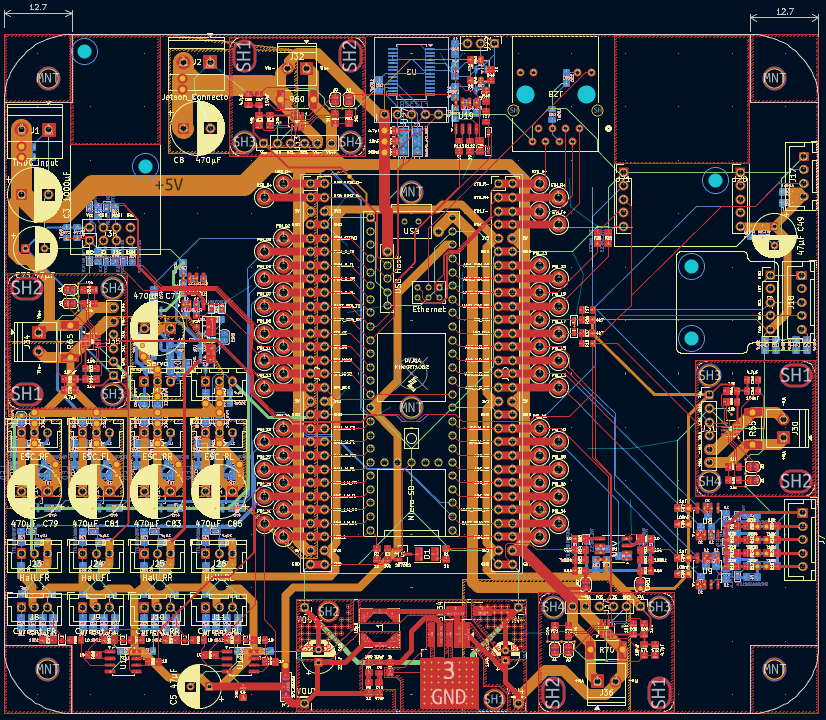
\includegraphics[width=1\textwidth, center]{images/design/kicad/board/v2/logic.png}
\end{figure}
\RmFigWS

The PCB makes use of four layers (explanations can be found \href{https://www.allpcb.com/blog/pcb-design/how-to-design-a-multi-layer-navigation-pcb-for-complex-systems.html}{here}):
\RmLstWS
\begin{enumerate}[nosep]
    \item Primary signal layer
    \item Ground plane
    \item Power plane (both 3V3 and 5V)
    \item Secondary signal layer
\end{enumerate}
\newpage
\subsubsection{Power board}
\RmLstWS
This is the board design of the power board:
\RmFigWS
\begin{figure}[h!]
    \caption{TruggySense power board PCB-design}
    \centering
    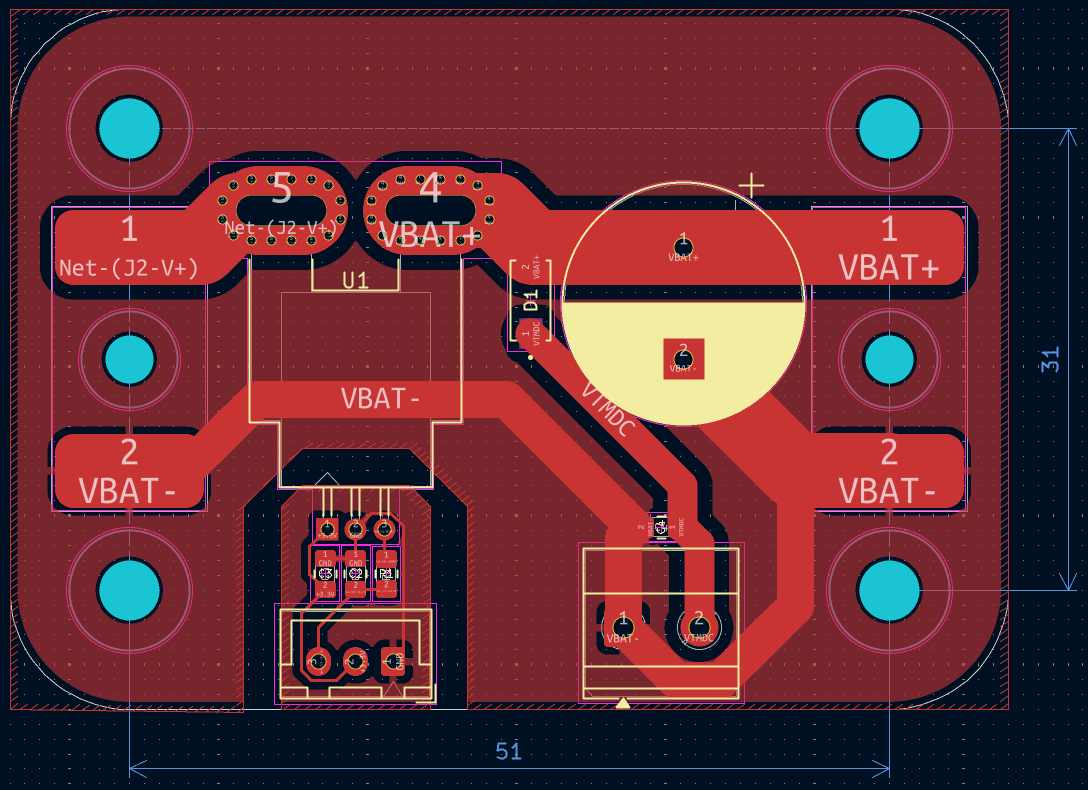
\includegraphics[width=0.333\textwidth, center]{images/design/kicad/board/v2/power.png}
\end{figure}
\RmFigWS

An important thing to note is that, to support a 200A current, the traces need a thickness of 389mm and copper thickness of 105µm.
This can be calculated using the following tools:
\RmLstWS
\begin{itemize}
    \item KiCAD calculation tool
    \item \href{https://www.advancedpcb.com/en-us/tools/trace-width-calculator/}{AdvancedPCb trace width calculator}
    \item \href{https://www.digikey.be/en/resources/conversion-calculators/conversion-calculator-pcb-trace-width}{DigiKey trace width calculator}
    \item \href{https://db-electronic.com/en/pcb-manufacturing_s54.htm}{Copperthickness conversion table}
\end{itemize}
\RmLstWS
Thus additional solid core copper wiring will be used to support this current.
\subsubsection{GPS board}
\RmLstWS
This is the board design of the GPS board:
\RmFigWS
\begin{figure}[h!]
    \caption{TruggySense GPS/GNSS board PCB-design}
    \centering
    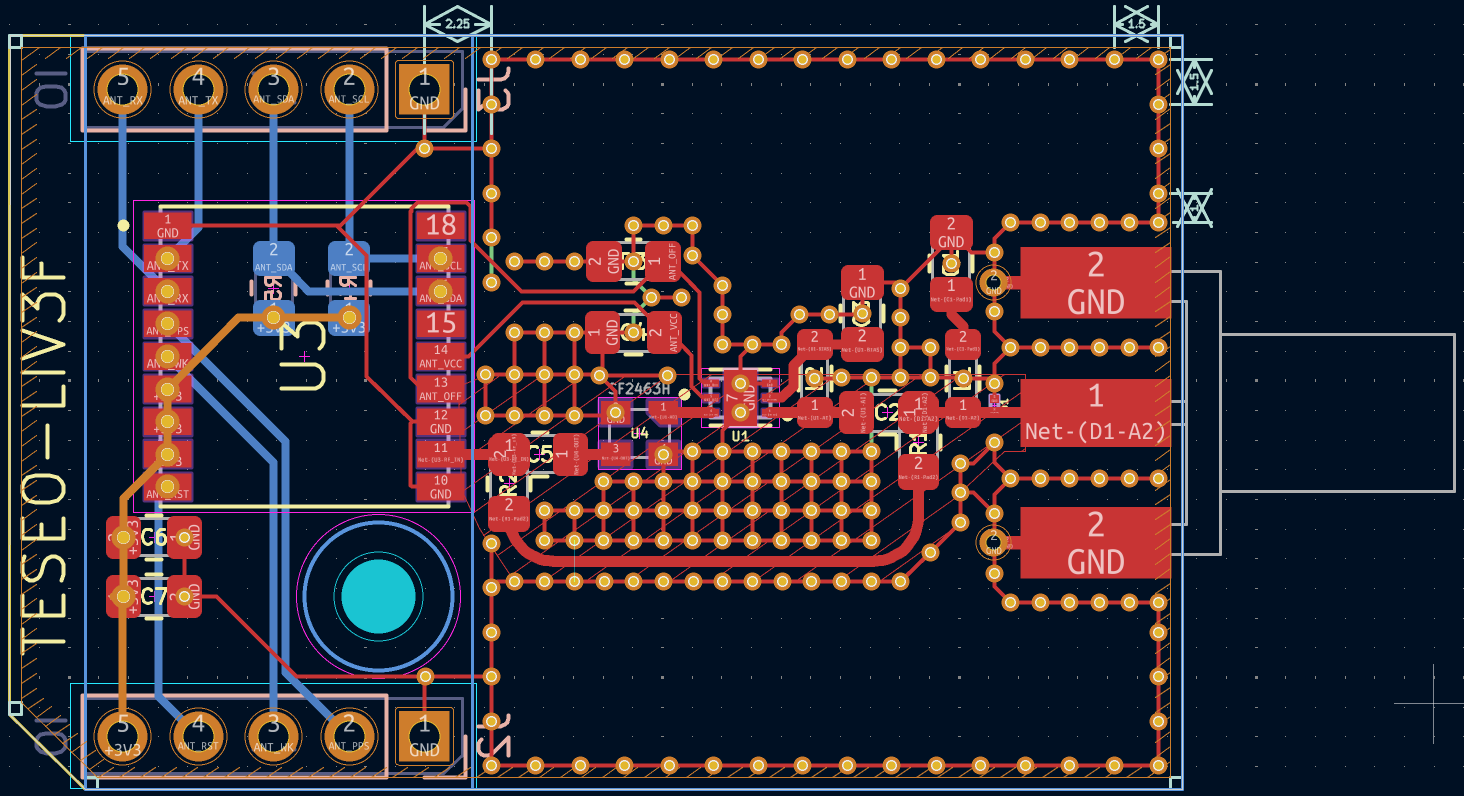
\includegraphics[width=0.5\textwidth, center]{images/design/kicad/board/v2/sensor_position.png}
\end{figure}
\RmFigWS

With the KiCAD calculation tool we can determine the size of the tracks so the input impedance is 50\si{\ohm}.
In this tool we need to select
\begin{itemize}
    \item High speed
    \item Transmission lines
    \item Transmission line type
    \item Coplaner wave guide w/ ground plane
\end{itemize}

Using the PCB editor's measuring tool, we know the length of the track is 22.1mm.
For the substrate we will use frequently used industry standard parameters: A thickness of 35µm and height of 480µm.
From the \href{URL}{datasheet of the TESEO-LIV3F} we know that the system works around 1575.4MHz.

The resulting width of the traces then must be 378µm.

Note that this board is also four layered, the same as the logic board.
\subsubsection{Temperature sensor board}
\RmLstWS
This is the board design of the temperature sensor board:
\RmFigWS
\begin{figure}[h!]
    \caption{TruggySense logic board PCB-design}
    \centering
    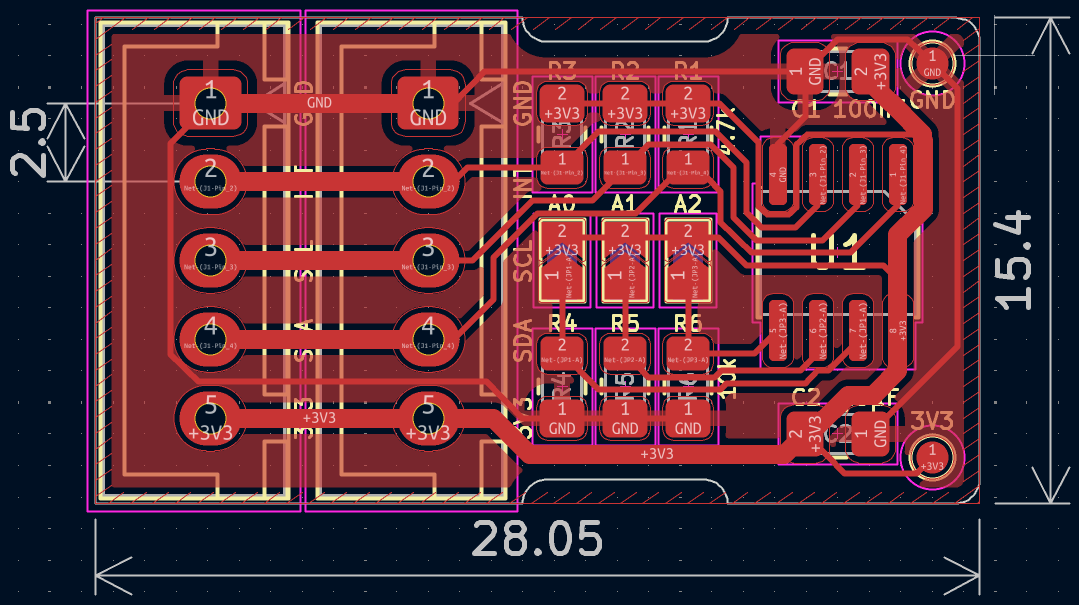
\includegraphics[width=0.5\textwidth, center]{images/design/kicad/board/v2/sensor_temperature.png}
\end{figure}
\RmFigWS
\subsubsection{Board recreations}
These components had low stock of the boards modules, but had high stock of their components.
Thus in case the boards aren't available, these boards will be implemented on the logic board.
\RmFigWS
\ImageComparison
    {Board recreations}
    {board_recreations}
    {{design/kicad/board/v2/ina219.png}/{Recreation of the INA219 board}
    /{design/kicad/board/v2/lm2596.png}/{Recreation of the LM2596 board}}
\RmFigWS
\subsubsection{Board layouts}
\RmLstWS
These boards had no footprint that could be found online, so one was made:
\RmFigWS
\ImageComparison
    {Board layouts}
    {board_layouts}
    {{design/kicad/board/v2/layout_nrf24l01.png}/{Recreation of the nRF24L01 board layout}
    /{design/kicad/board/v2/layout_pim448.png}/{Recreation of the PIM448 board layout}}
\RmFigWS
\newpage
\section{Assembly}
\subsection{Board assemblies}
\ImageComparison
    {TruggySense assembled logic board}
    {logic_board_assembly}
    {{design/assembly/v2/logic_board_top.png}/{Logic board top}
    /{design/assembly/v2/logic_board_bottom.png}/{Logic board bottom}}
\RmFigWS
\ImageComparison
    {TruggySense assembled power board}
    {power_board_assembly}
    {{design/assembly/v2/power_board_top.png}/{Power board top}
    /{design/assembly/v2/power_board_bottom.png}/{Power board bottom}}
\RmFigWS
Note that solid copper wires, with a core surface of 2.5mm², should be used to connect the positive and negative terminals of the EC5 connectors.

\begin{figure}[h!]
    \centering
    \begin{minipage}[c]{0.4\textwidth}
        \centering
        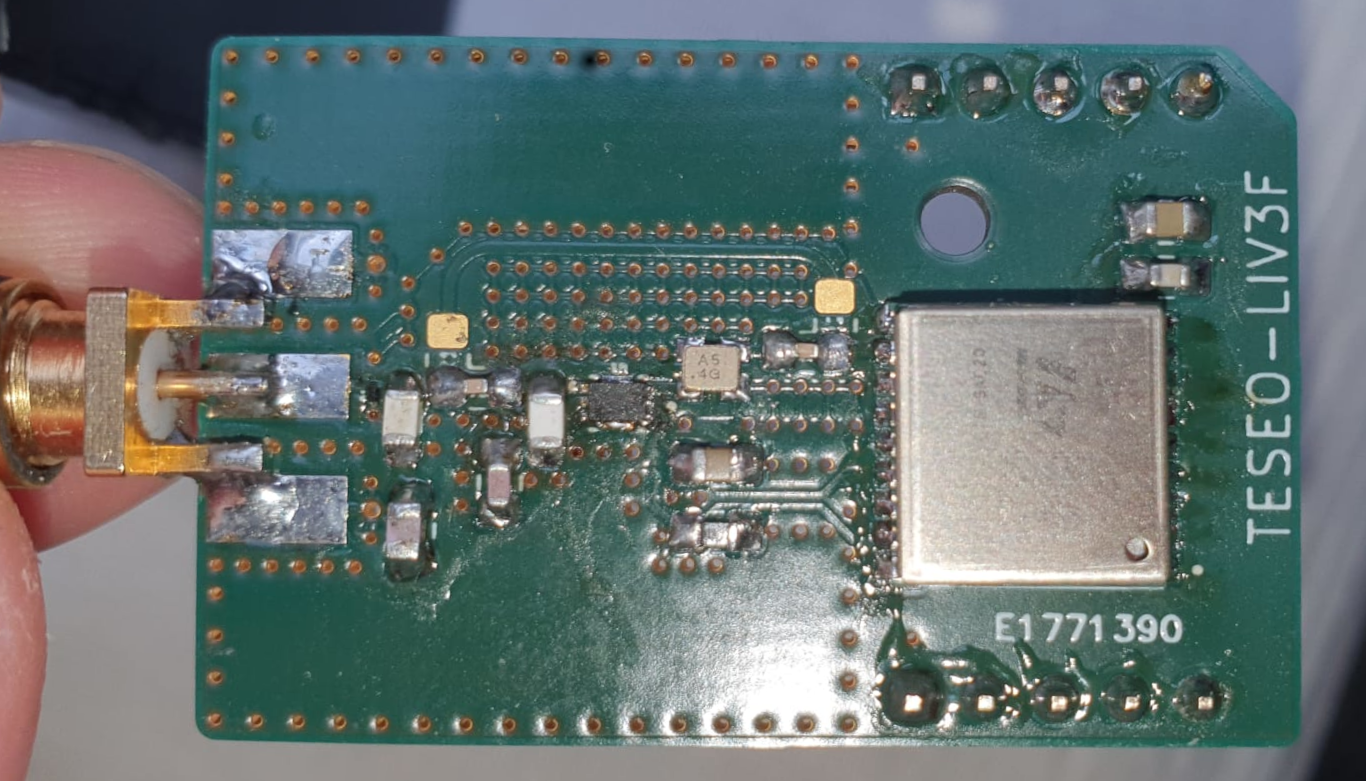
\includegraphics[width=\textwidth]{images/design/assembly/v2/position_board.png}
        \caption{TruggySense assembled GNSS/GPS board}
    \end{minipage}
    \hspace{1.5cm}
    \begin{minipage}[c]{0.33\textwidth}
        \centering
        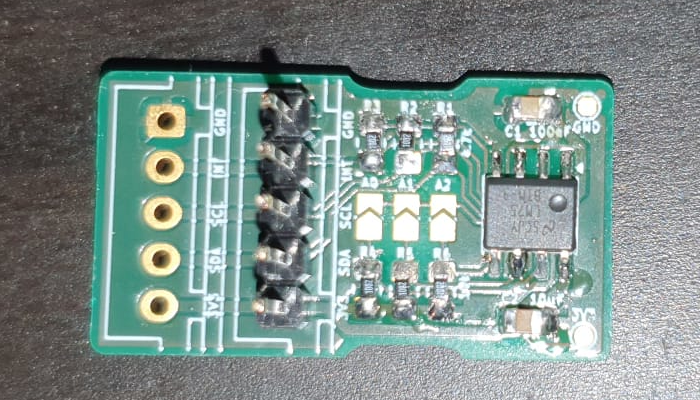
\includegraphics[width=\textwidth]{images/design/assembly/v2/temperature_sensor.png}
        \caption{TruggySense assembled temperature sensor}
    \end{minipage}
\end{figure}
\RmFigWS
Note that the address of the temperature sensor module increases by shorting the address pads.
\newpage
\subsection{PCB faults}
These are the problems of the prototype boards:
\begin{table}[h!]
    \centering
    \caption{Faults of the prototype PCBs}
    \centering
    \begin{tabular}{p{0.13\textwidth} p{0.85\textwidth}}
        \toprule
            \textbf{Board} & \textbf{Faults} \\
        \midrule
            \raisebox{-3.33mm}{Logic:} & 
            \begin{itemize}
                \item The antenna of the GNSS/GPS module cannot be attached, while the HLC is attached, due to limited space.
                \item The ethernet pins of the LLC can only be attached if the teensy board is directly soldered to the PCB.
                      Thus making ethernet connectivity impossible.
                \item The option to connect the teensy's USB host pins should be removed since the LLC should never be the host device.
                \item The PCB is to large to allow all modules on the vehicle.
                      Besides that a large open gap is still present on the right side of the PCB.
                \item The extra USB port obstructs the LLC's usb port.
                \item The buffer circuits only have a operating range between 0.65V and 2.65V.
                      Thus they should be removed.
                \item The ADC pads for the 3.3V and 5V are by default disconnected.
                      They should be connected by default.
                \item The FlySky module functions on 5V, but gives a uart signal of max 3.3V.
                \item The RS232FL circuit doesn't function.
                \item TLE4095 uses 5V logic.
                \item Pins 28 to 31 aren't analogue inputs, thus the high current sensors do not work.
                \item The TVS diodes interfere with the digital protocol signals (UART, SPI, I²C).
            \end{itemize} \\
            \raisebox{-3.33mm}{Power:} & 
            \begin{itemize}
                \item Only supports 1 motor.
                \item There is no clear line for the battery's positive and negative terminals to be connected to the needed modules (via a solid core copper wire).
                \item The high current sensor can only handle up to 10nF capacitors on its line, lest it will malfunction.
                \item The 5V logic of the high current sensor is more reliable.
                      A 56kOhm and 100kOhm voltage divider was added to support this logic.
            \end{itemize} \\
            \raisebox{-3.33mm}{GNSS/GPS:} & 
            \begin{itemize}
                \item The board is to thick for the antenna.
                      Use through holes next time.
                \item The board is designed for a passive antennas, but these are hard to find for GNSS/GPS's.
                      Since the board doesn't support active antennas, the board is unusable.
            \end{itemize} \\
            \raisebox{-3.33mm}{Temperature:} & 
            \begin{itemize}
                \item The sensor is on the same side as the components.
                      To make sure none of the components's pads make contact with metal, and short, Kapton tape was added.
                      Change te module so that the sensor is on the opposite side of the components.
            \end{itemize} \\
        \bottomrule
    \end{tabular}
\end{table}
\newpage
\subsection{PCB fixes}
The following images illustrate the components that were not needed or malfunctioned.
The red crosses cover components/circuits that can be removed, while keeping the system functional.
The blue lines represent, shorts that have to be soldered to make the system functional.
Finally, the white squares represent the pin headers to connect certain modules to:
\begin{enumerate}
    \item The ACS756 high current sensor is connected to pin 22 (analog pin).
    \item The GY-NEO6M GPS is connected to the UART 5 pins.
    \item The BNO085 IMU is connected to the I²C pins.
    \item The FS-X6B remote control receiver is connected to the UART 8 pins.
\end{enumerate}
Note that all these modules require a 5V souce.
\ImageComparison
    {TruggySense altered logic board}
    {altered_logic_board_assembly}
    {{design/assembly/edits/logic_board_top.png}/{Logic board top}
    /{design/assembly/edits/logic_board_bottom.png}/{Logic board bottom}}
\RmFigWS

A voltage devider was added to the circuit, with $R_1 = 56k\Omega$ and $R_2 = 100k\Omega$.
\begin{figure}[h!]
    \caption{TruggySense altered supply board}
    \centering
    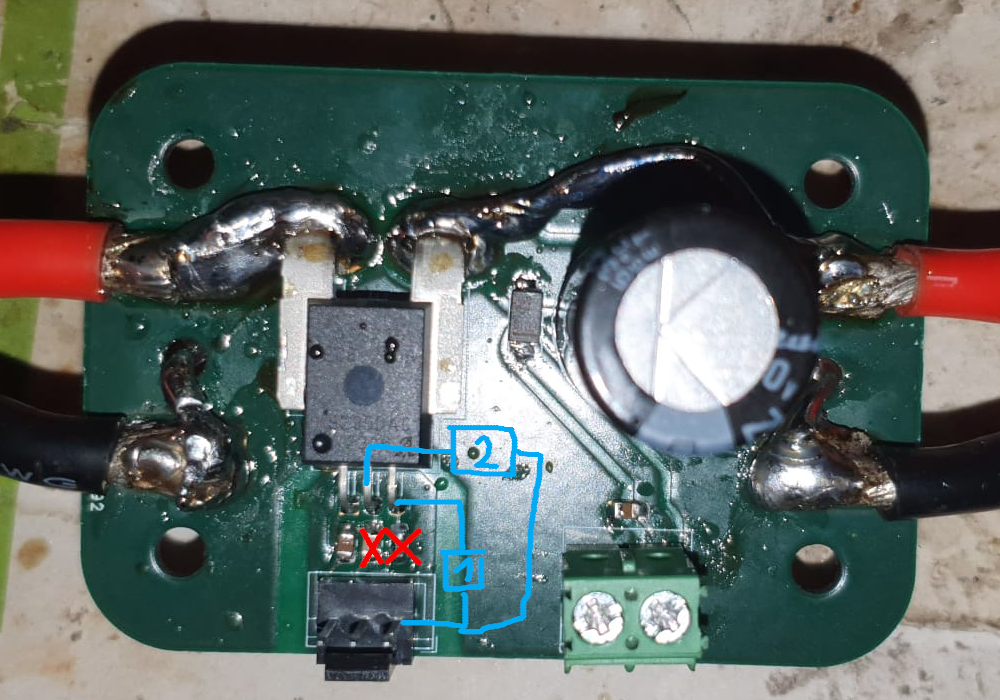
\includegraphics[width=0.4\textwidth, center]{images/design/assembly/edits/power_board.png}
\end{figure}
\clearpage

Add Kapton tape to the temperature sensor board to make sure that no short-circuits occur when placed against metal.
Use angled GPIO headers on the back of the board to daisy chain the modules together.
\ImageComparison
    {TruggySense altered temperature sensor board}
    {altered_temperature_board_assembly}
    {{design/assembly/edits/temperature_sensor_top.png}/{Temperature sensor board top}
    /{design/assembly/edits/temperature_sensor_bottom.png}/{Temperature sensor bottom}}
\subsection{BOM}
\label{sec:kicad_bom}
To install the plugin for the interactive BOM. Go to:

Main KiCAD screen \textgreater~Tools Tab \textgreater~Plugin and content manager \textgreater~Interactive Html BOM

Click: "Install" then "Apply Pending Changes"

Click here to see the interactive BOM:
\begin{itemize}
    \item \href{../../cad/KiCAD/v2/1_logic_board/bom/ibom.html}{Logic board}
    \item \href{../../cad/KiCAD/v2/2_power_board/bom/ibom.html}{Power board}
    \item \href{../../cad/KiCAD/v2/sensor_position/bom/ibom.html}{GPS/GNSS board}
    \item \href{../../cad/KiCAD/v2/sensor_temperature/bom/ibom.html}{Temperature sensor}
\end{itemize}

Note that the GPS has been replaced by the \href{https://www.otronic.nl/nl/gps-module-gy-neo6mv2-met-antenne-voor-a-140568422.html}{\textbf{GY-NEO6MV2}} and that the IMU by the \href{https://www.digikey.be/nl/products/detail/adafruit-industries-llc/4754/13426653?s=N4IgTCBcDaIEIDkDyAGAHAVhAXQL5A}{\textbf{BNO085}}.

These are the components to not add:
\begin{table}[h!]
    \centering
    \caption{Components that should be excluded from the BOM.}
    \begin{tabular}{p{1cm} p{2.2cm} p{7cm} p{3.5cm}}
        \toprule
            \textbf{Board} & \textbf{Component} & \textbf{Reference} & \textbf{Reason} \\
        \midrule
            Logic   & Capacitor   & C3.1, 3.2, C11, C12, C65, C66, C67, C68, C69, C70, C71, C72 & Included on dev-board \\
            Logic   & Connector   & J30, J32, J34, J36 & Included on dev-board \\
            Logic   & Diode       & D2 & Included on dev-board \\
            Logic   & Inductor    & L1 & Included on dev-board \\
            Logic   & Resistor    & R2.1, R2.2, R6, R53, R54, R55, R56, R57, R58, R59, R60, R61, R62, R63, R64, R65, R66, R67, R68, R69, R70, R71, R72 & Included on dev-board \\
            Logic   & Sensor      & U2, U4, U5, U6, U7 & Included on dev-board \\
        \midrule
            Logic   & Capacitor   & C25, C26, C27, C28, C29, C30, C31, C32, C33, C34, C35, C36, C37, C38, C39, C40, C45, C46, C47, C48, C61, C62, C63, C64, C86, C87, C88, C89, C92, C93, C94, C95, C96, C97, C98, C99 & Broken circuit \\
            Logic   & Connector   & J8, J9, J10, J11, J19, J20, J21, J22, J27, J29 & Broken circuit \\
            Logic   & Diode       & D3, D10, D11, D12, D13, D19, D20, D21, D22, D23, D24, D25, D26, D27, D28, D29, D30, D31 & Broken circuit \\
            Logic   & Fuse        & F7, F8, F9, F10, F23, F24, F25, F26, F27, F28 & Broken circuit \\
            Logic   & Module      & U3, U8, U9, U10, U11, U12, U18, U19 & Broken circuit \\
            Logic   & Resistor    & R25, R26, R27, R28, R29, R30, R31, R32, R33, R34, R35, R36, R39, R40, R41 R42, R43, R44, R45, R46, R47, R52, R73, R74, R75, R76, R77, R78, R79, R80, R81, R82, R83, R84, R85, R86, R87, R88, R89, R90, R91, R92, R108, R109, R110, R111, R112, R113, R114, R115 & Broken circuit \\
            Logic   & Transistor  & Q2, Q3, Q4, Q5 & Broken circuit \\
        \midrule
            Power   & Capacitor   & C2 & Broken circuit \\
            Power   & Resistor    & R1 & Broken circuit \\
        \midrule
            GPS     & Capacitor   & C1, C2, C3, C4, C5, C6, C7 & Broken circuit \\
            GPS     & Connector   & J1, J2, J3 & Broken circuit \\
            GPS     & Diode       & D1 & Broken circuit \\
            GPS     & Inductor    & L1, L2 & Broken circuit \\
            GPS     & Module      & U1, U3, U4 & Broken circuit \\
            GPS     & Resistor    & R1, R2, R3, R4, R5 & Broken circuit \\
        \bottomrule
    \end{tabular}
    \label{tab:exclude_from_bom}
\end{table}

This is the BOM with the components above removed:
\Needspace{10\baselineskip}     % Set table not prematurely overflow to next page
\begin{table}[h!]
    \centering
    \caption{Bill of materials of the TruggySense v2}
    \begin{adjustbox}{max width=\textwidth, max height=1\textheight}
        \begin{tabular}{l r c c}
            \toprule
                \textbf{Component} & \textbf{Value} & \textbf{Qty} & \textbf{Footprint} \\
            \midrule
                \csvreader[
                    head to column names,
                    late after line=\\,
                ]{./databases/design/bom/prototype.csv}{}{
                    \href{\PurchaseLink}{\Component} & 
                    \href{\PurchaseLink}{\Value} &
                    \href{\PurchaseLink}{\Qty} & 
                    \Footprint
                }
            \bottomrule
        \end{tabular}
    \end{adjustbox}
    \label{tab:bill_of_materials}
\end{table}
\clearpage
\newpage
\section{FreeCAD}
FreeCAD 1.0.0 was used for the 3D-designs.
The guide below will show how to install FreeCAD and showcase the base functionalities.
\subsection{Guide}
\label{sec:freecad_guide}
\subsubsection{Install FreeCAD}
The installation for Windows can be found using \href{https://www.freecad.org/downloads.php}{this link}.

The installation for Linux (Debian and Ubuntu) can be done using the following commands:
\begin{lstlisting}[style=cmd]
# Install KiCad:
    sudo apt update && sudo apt install -t freecad

# Verify success:
    freecad --version
\end{lstlisting}
\subsubsection{Create a base}
To create a project follow this \href{https://www.youtube.com/watch?v=E14m5hf6Pvo&t=45s}{guide}.
The base steps are as follows:
\RmLstWS
\begin{enumerate}[nosep]
    \item Create a project
    \item Create a sketch
    \item Select the XY-plane
    \item Create the base form off the object (we will subtract parts from it later)
    \item Add constraints (if all lines are green everything is ok)
    \item Exit the sketch and select "PAD"
    \item Select the face you want to edit, and create a new sketch (this will align itself the right way)
\end{enumerate}
\RmLstWS
Make sure to reduce the Degrees of Freedom (DoF), of the sketch, as much as possible.
\subsection{Designs}
\subsubsection{Unchanged designs}
These are the designs that were taken from the TSV1, without any changes:
\RmFigWS
\begin{figure}[h!]
    \caption{Rear mount for the base plate}
    \centering
    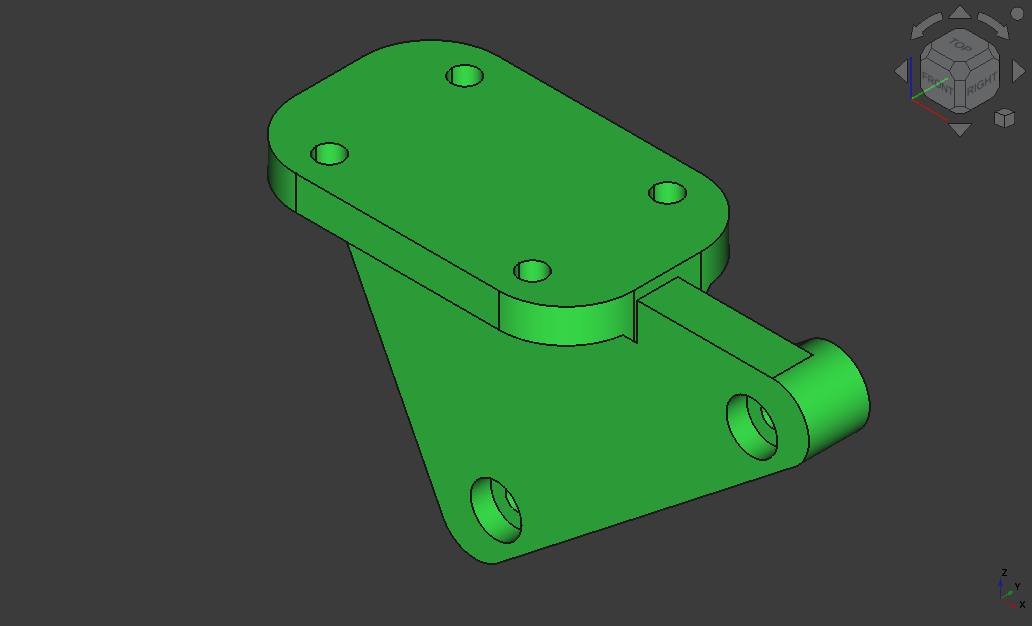
\includegraphics[width=0.5\textwidth, center]{images/design/freecad/renders/v1/rear_mount.png}
\end{figure}
\newpage

\begin{figure}[h!]
    \caption{Encoder ring at the wheel base}
    \centering
    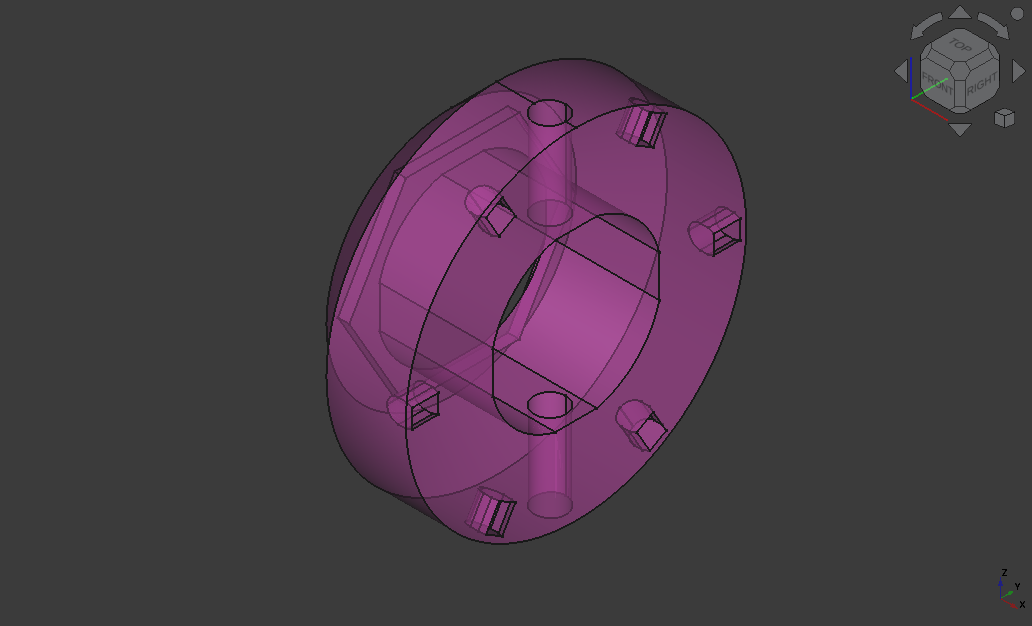
\includegraphics[width=0.5\textwidth, center]{images/design/freecad/renders/v1/encoder_ring.png}
\end{figure}
\RmFigWS

When opening this document, the amount of magnet slots (and with that precision) can be altered by changing the variable under:
wheel\_encoder \textgreater~encoder\_rin \textgreater~encoder\_mag \textgreater~PolarPattern.

\RmFigWS
\ImageComparison
    {Encoder sensor holder}
    {encoder_holder_design}
    {{design/freecad/renders/v1/front_encoder.png}/{Front holder (TruggySense v1)}
    /{design/freecad/renders/v1/rear_encoder.png}/{Rear holder (TruggySense v1)}}
\RmFigWS

Note that these encoder parts should disappear when the custom made wheels/motors are designed.

\begin{figure}[h!]
    \caption{Motor mechanism}
    \centering
    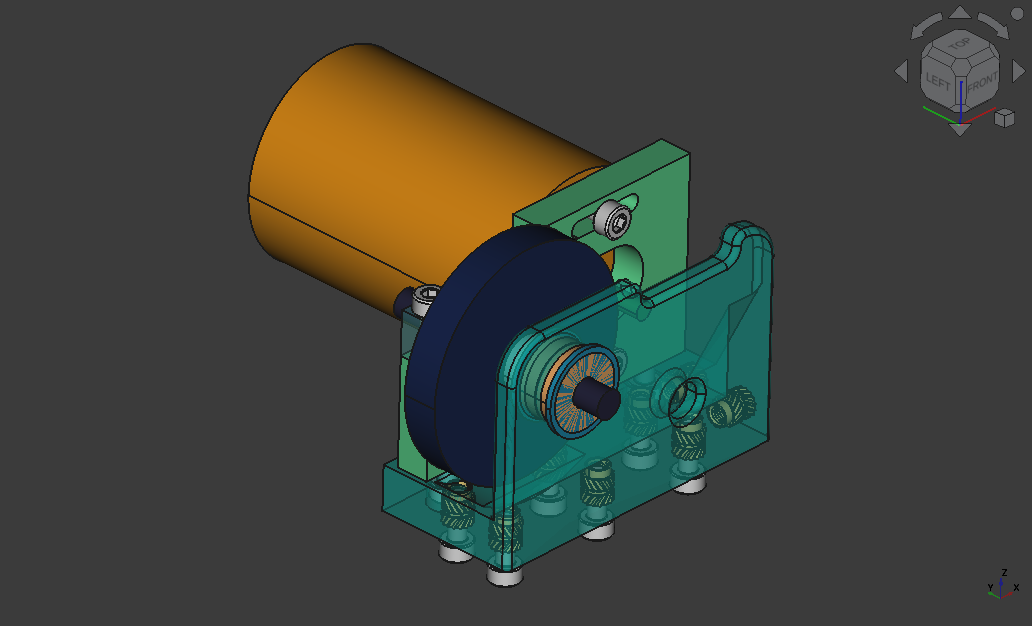
\includegraphics[width=0.5\textwidth, center]{images/design/freecad/renders/v1/motor_mechanism.png}
\end{figure}
\RmFigWS

Note that the motor mount parts should disappear when the custom made wheels/motors are designed.

\begin{figure}[h!]
    \caption{Casing for the RC communication module}
    \centering
    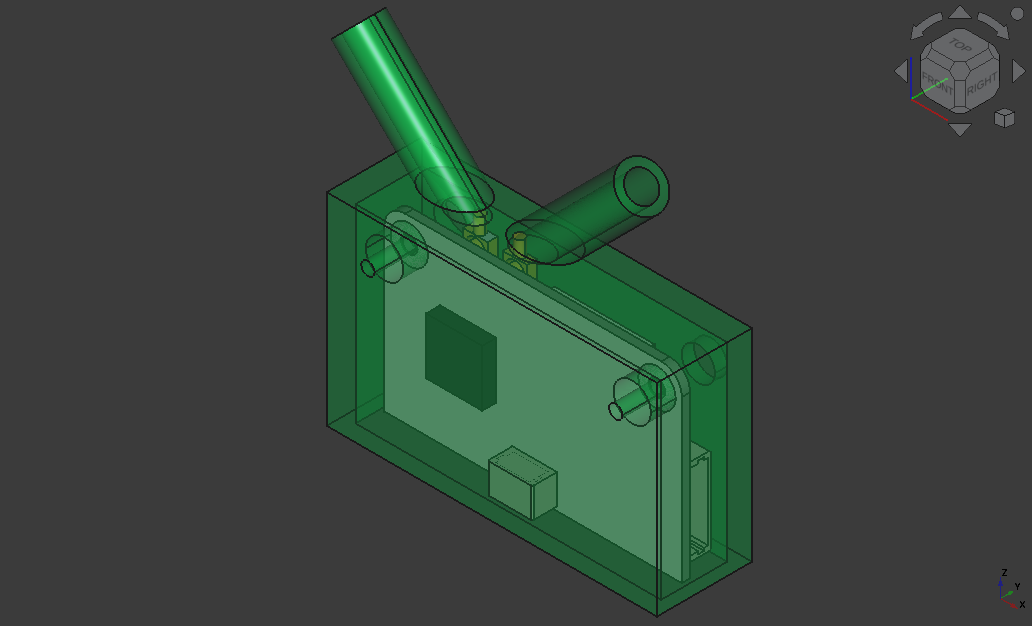
\includegraphics[width=0.5\textwidth, center]{images/design/freecad/renders/v1/x6b_case.png}
\end{figure}
\begin{figure}[h!]
    \caption{Cable clamp}
    \centering
    
\includegraphics[width=0.5\textwidth, center]{images/design/freecad/renders/v1/cable_manager.png}
\end{figure}
\RmFigWS
\begin{figure}[h!]
    \caption{Nvidia Jeston Nano casing lid}
    \centering
    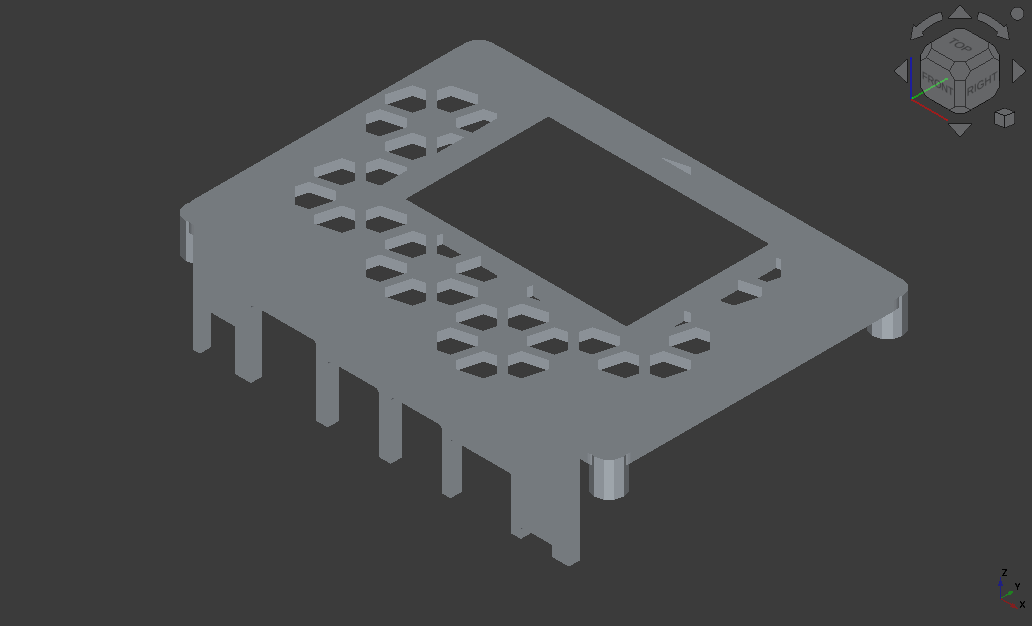
\includegraphics[width=0.5\textwidth, center]{images/design/freecad/renders/v1/jetson_lid.png}
\end{figure}
\RmFigWS
\newpage
\subsubsection{Altered designs}
These are the designs that were taken from the TSV1, but were altered:
\RmFigWS
\ImageComparison
    {Nvidia Jeston Nano casing}
    {jetson_case_design}
    {{design/freecad/renders/v1/jetson_case.png}/{TruggySense v1}
    /{design/freecad/renders/v2/jetson_case.png}/{TruggySense v2}}

\ImageComparison
    {Tube clamps}
    {tube_clamp_design}
    {{design/freecad/renders/v1/tube_clamp_wide.png}/{Wide tube clamp (TruggySense v1)}
    /{design/freecad/renders/v2/tube_clamp_wide.png}/{Wide tube clamp (TruggySense v2)},
    {design/freecad/renders/v1/tube_clamp_short.png}/{Short tube clamp (TruggySense v1)}
    /{design/freecad/renders/v2/tube_clamp_long.png}/{Long tube clamp (TruggySense v2)}}

\ImageComparison
    {Base plate}
    {base_plate_design}
    {{design/freecad/renders/v1/base_plate.png}/{TruggySense v1}
    /{design/freecad/renders/v2/base_plate.png}/{TruggySense v2}}

\newpage
\subsubsection{New designs}
These are the new designs for the TruggySense v2:
\RmFigWS
\begin{figure}[h!]
    \caption{TMDC 20-2411 holder}
    \centering
    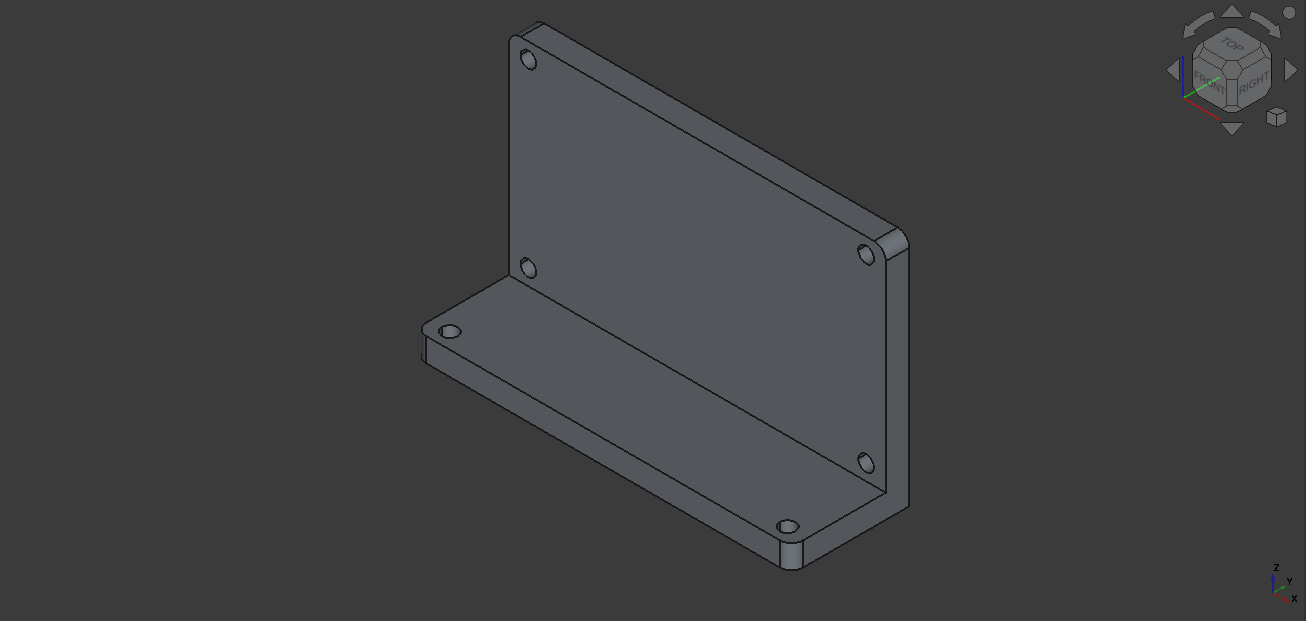
\includegraphics[width=0.5\textwidth, center]{images/design/freecad/renders/v2/tmdc_holder.png}
\end{figure}
\newpage
\section{Metalcut}
\label{sec:metalcut_guide}
Laser cutting can be done at the University of Antwerp G.Z.0.62.

The material used is 6mm thick Acrylic/PMMA.
To cut this we must first render the .dxf file in a program called \textbf{Metalcut}.
Once the file is imported look at the right side of the screen and enter the following values:
\RmLstWS\RmLstWS\RmLstWS
\begin{itemize}
    \item Power 85\%
    \item Speed 12mm/s
\end{itemize}
\RmLstWS
Note that these values change depending on the material and its thickness.
For any material located in the room, the settings have been noted in an excel file that is either located on the computer or in the browser.

Before we export the file we need to simulate it.
If there is any overlap or unusual cutting, follow these steps:
\begin{multicols}{5}
    \RmLstWS
    \begin{itemize}[label={}]
        \item \small Select all
        \IconItem{metalcut/icons/delete_overlap}{\small Delete overlap}
        \IconItem{metalcut/icons/combine_curve}{\small Combine curve}
        \IconItem{metalcut/icons/cut_optimize}{\small Cut optimize}
        \IconItem{metalcut/icons/simulate}{\small Simulate}
    \end{itemize}
\end{multicols}
\RmLstWS\RmLstWS
If the simulation looks good your can export the file to a ".rd".

Follow these steps for the laser cutter:
\RmLstWS
\begin{itemize}
    \item On the panel:
    \begin{itemize}
        \item Put USB in UDisk slot
        \item Turn big red twisting knob
    \end{itemize}
    \item On the menu:
    \begin{itemize}
        \item Press file
        \item Press uDisk
        \item Load file in mem
        (If file name is already present, clear local mem files)
    \end{itemize}
    \item On the panel:
    \begin{itemize}
        \item Press the reset button
    \end{itemize}
    \item On the menu:
    \begin{itemize}
        \item Go to main menu
        \item Put laser in top right corner (= origin) using the arrow buttons.
        \item Adjust the height
    \end{itemize}
    \item On the panel:
    \begin{itemize}
        \item Turn on the laser power
    \end{itemize}
    \item On the menu:
    \begin{itemize}
        \item Press start
    \end{itemize}
    \item \textcolor{red}{\textbf{!!! Keep watch over the cut until completion. !!!}}
    \item Check the cut without moving the plate.
    If the cut hasn't completely gone through, re-run the program.
\end{itemize}
\RmFigWS
\ImageComparison
    {Laser cutter}
    {laser_cutter}
    {{design/metalcut/laser_cutter_panel.png}/{Laser cutter panel}
    /{design/metalcut/laser_cutter_menu.png}/{Laser cutter menu}}
\newpage
\section{Structural assembly}
\subsection{Wheel assembly}
The first thing that needs modification, are the wheels.
To detach the wheel, use a 17mm wrench to remove the hub cap.
Afterwards, install the new wheel hubs, with a 10mm extension, by removing the hub pin (indicated by the blue arrow).
\ImageComparison
    {Wheel hub assembly}
    {wheel_hub}
    {{design/assembly/steps/wheel/1.png}/{Wheel}
    /{design/assembly/steps/wheel/2.png}/{Wheel hub}}

The images below indicate how the encoder should be mounted onto the wheel hub.
\begin{figure}[h!]
    \centering
    \caption{Encoder assembly}
    \begin{subfigure}{0.32\textwidth}
        \centering
        
\includegraphics[width=\textwidth]{images/design/assembly/steps/wheel/3.png}
        \caption{Render of the full encoder assembly}
    \end{subfigure}
    \hfill
    \begin{subfigure}{0.32\textwidth}
        \centering
        
\includegraphics[width=\textwidth]{images/design/assembly/steps/wheel/4.png}
        \caption{Sensor placement in holder}
    \end{subfigure}
    \hfill
    \begin{subfigure}{0.32\textwidth}
        \centering
        
\includegraphics[width=\textwidth]{images/design/assembly/steps/wheel/5.png}
        \caption{Full encoder assembly}
    \end{subfigure}
\end{figure}

Note that the front and back use slightly different sensor holder.
\newpage
\subsection{Base plate assembly}
Mount the bottom of the Jetson case to the base plate, using the screws indicated by the arrows.
\begin{figure}[h!]
    \caption{Jeston case mounted to base plate}
    \centering
    
\includegraphics[width=0.6\textwidth, center]{images/design/assembly/steps/plate/1.png}
\end{figure}

Mount the Jetson to its case, and the \href{https://makerworld.com/en/models/48790-gps-gy-gps6mv2-module-case-neo-6m#profileId-107595}{\textbf{GPS}} and \href{https://www.thingiverse.com/thing:6326703}{\textbf{IMU}} to the jetson lid, using the screws indicated by the arrows.
\begin{figure}[h!]
    \caption{Jetson mounted to the case, and the GPS and IMU mounted to the lid}
    \centering
    
\includegraphics[width=0.6\textwidth, center]{images/design/assembly/steps/plate/2.png}
\end{figure}

Place the Jetson case lid, to the rest of the casing.
Attach the temperature sensor in the heatsink of the Jetson, while keeping space for the fan.
Then mount the fan, fasten the lid, and attach the logic board to the base plate, using the screws indicated by the arrows.
\begin{figure}[h!]
    \caption{Full mount of the Jetson case and logic board}
    \centering
    
\includegraphics[width=0.6\textwidth, center]{images/design/assembly/steps/plate/3.png}
\end{figure}

\newpage
\subsection{Base plate mounts assembly}
There are holes located at the rear of the chassis that could be use to attach a mounting point for the base plate.
\begin{figure}[h!]
    \centering
    \caption{Rear base plate mount}
    \begin{subfigure}{0.32\textwidth}
        \centering
        
\includegraphics[width=\textwidth]{images/design/assembly/steps/mount/1.png}
        \caption{Chassis without mount}
    \end{subfigure}
    \begin{subfigure}{0.32\textwidth}
        \centering
        
\includegraphics[width=\textwidth]{images/design/assembly/steps/mount/2.png}
        \caption{Chassis with mount}
    \end{subfigure}
\end{figure}

Clamps can then be used to attach the base plate to the center axis of the chassis.
\begin{figure}[h!]
    \caption{The brackets attachted to the main axis of the chassis}
    \centering
    
\includegraphics[width=0.6\textwidth, center]{images/design/assembly/steps/mount/3.png}
\end{figure}

\subsection{Remote control receiver mounting}
Attach the remote control receiver to the front of the chassis.
\begin{figure}[h!]
    \caption{Remote control receiver mounting}
    \centering
    
\includegraphics[width=0.4\textwidth, center]{images/design/assembly/steps/other/1.png}
\end{figure}

\newpage
\subsection{Car assembly}
Place the battery into its slot and attach the temperature sensors on the ESC, motor, servo, and battery, as indicated by the arrows.
\begin{figure}[h!]
    \caption{TruggySense chassis construction}
    \centering
    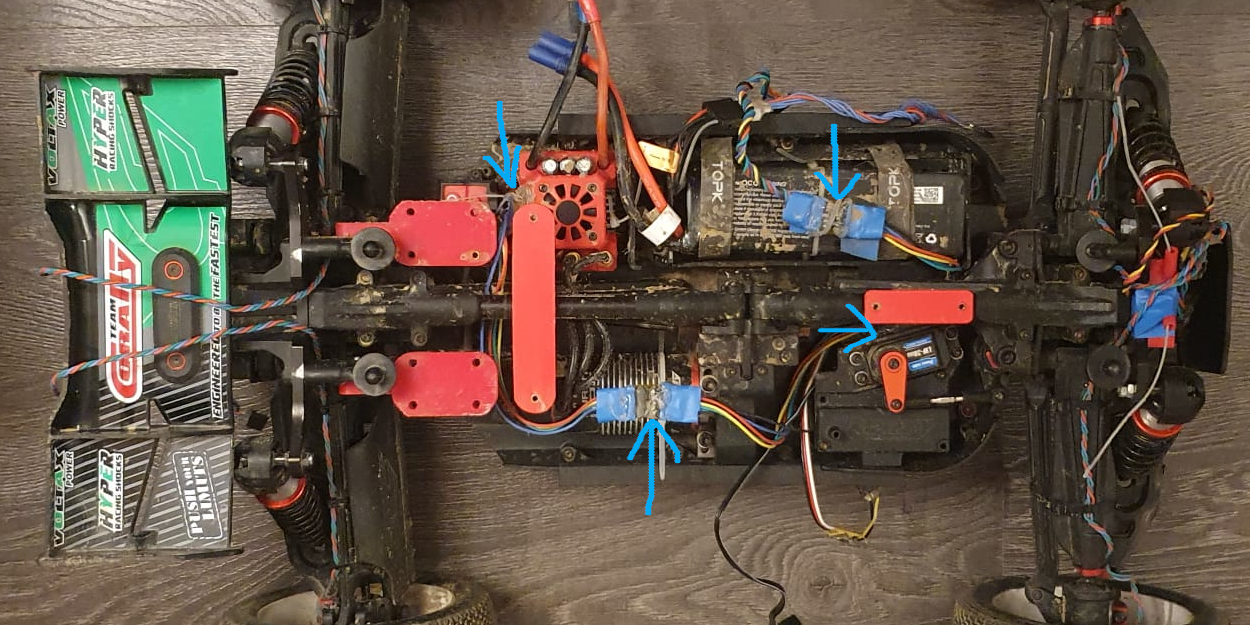
\includegraphics[width=0.6\textwidth, center]{images/design/assembly/steps/car/1.png}
\end{figure}

Afterwards, the base can be slided onto the brackets.
\begin{figure}[h!]
    \caption{TruggySense chassis with base plate assembly}
    \centering
    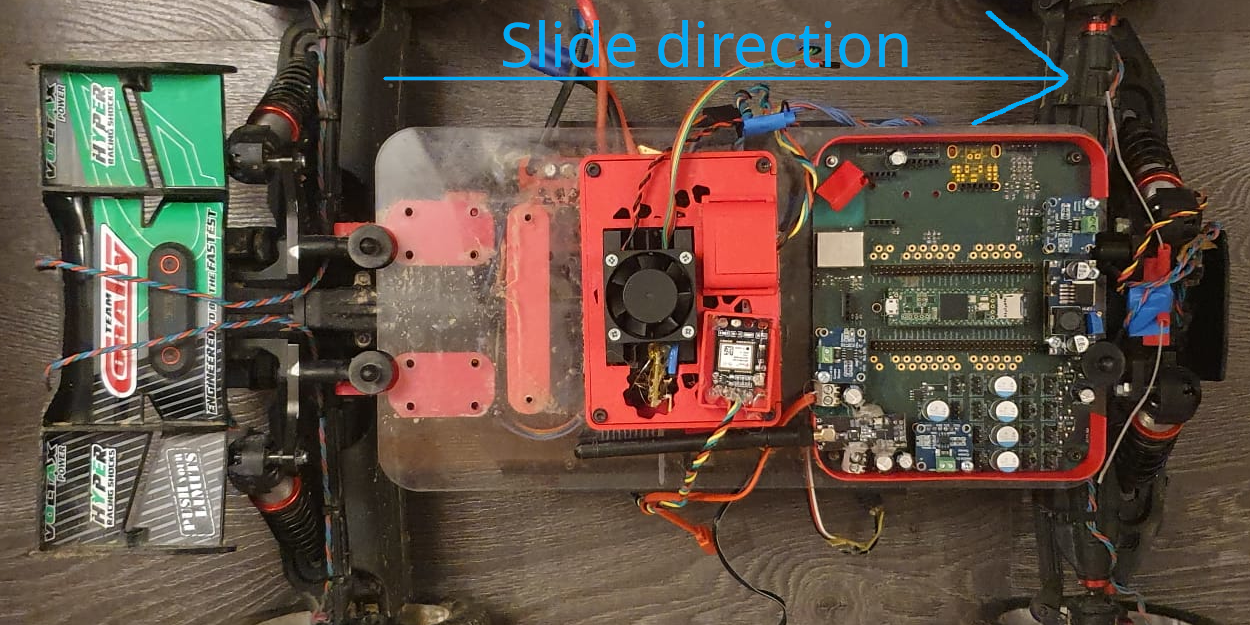
\includegraphics[width=0.6\textwidth, center]{images/design/assembly/steps/car/2.png}
\end{figure}

Fixate the base plate by attaching the screws, as indicated by the arrows.
\begin{figure}[h!]
    \caption{Fixated the base plate to the chassis}
    \centering
    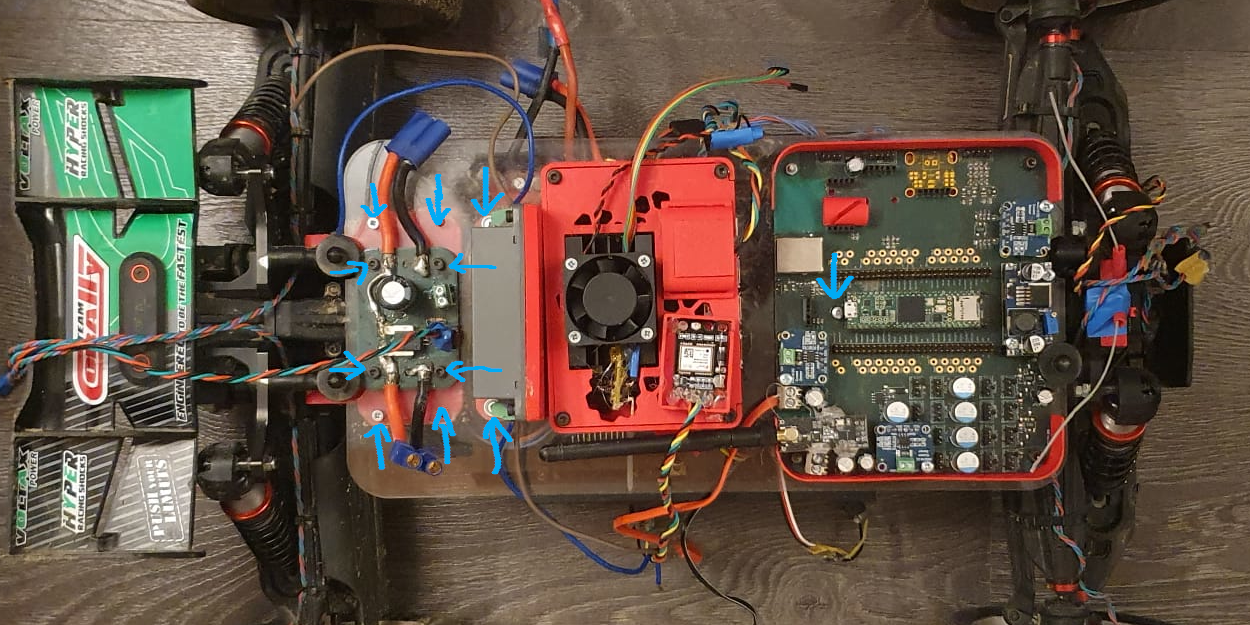
\includegraphics[width=0.6\textwidth, center]{images/design/assembly/steps/car/3.png}
\end{figure}

\newpage
Connect all cables to their designated pins.
For any alteration, see Fig.~\ref{fig:altered_logic_board_assembly}.
\begin{figure}[h!]
    \caption{Cables connected}
    \centering
    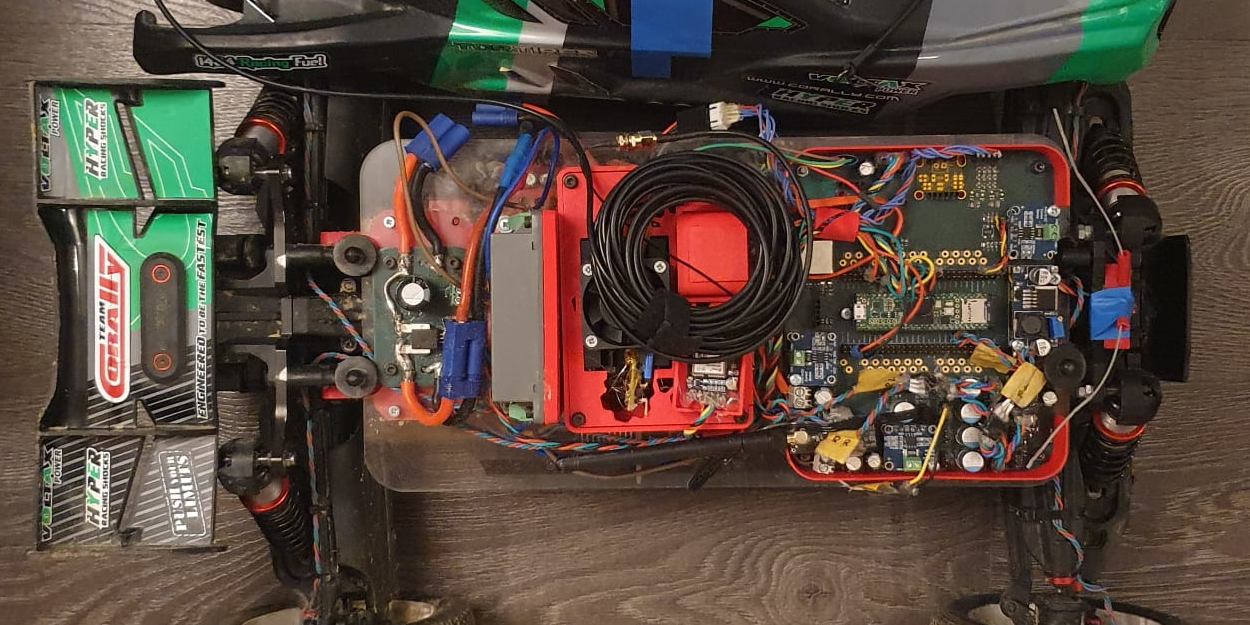
\includegraphics[width=0.6\textwidth, center]{images/design/assembly/steps/car/4.png}
\end{figure}

Attach the lid using the mounting pins, as indicated bu the arrows.
Start with the rear of the cart.
\begin{figure}[h!]
    \caption{Lid attached}
    \centering
    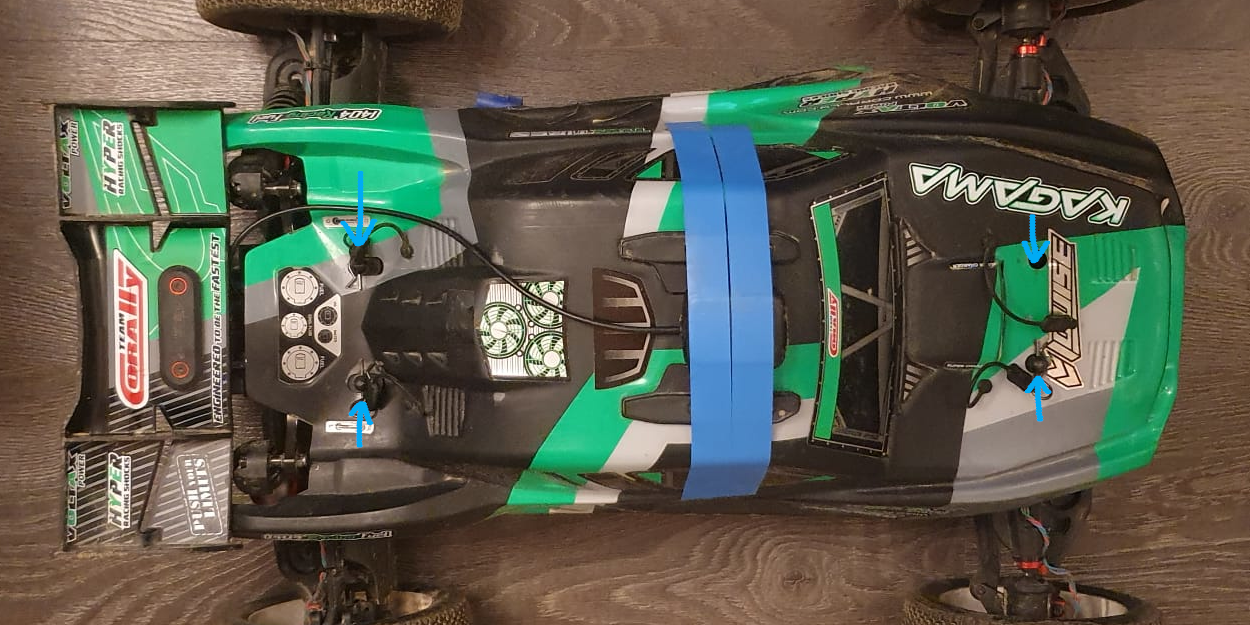
\includegraphics[width=0.6\textwidth, center]{images/design/assembly/steps/car/5.png}
\end{figure}

\chapter{Finalized Design}          % ---------------------- Finalized design ----------------------
\section{Logical design}
\RmFigWS
\begin{figure}[h!]
    \caption{TruggySense logic interaction between modules}
    \centering
    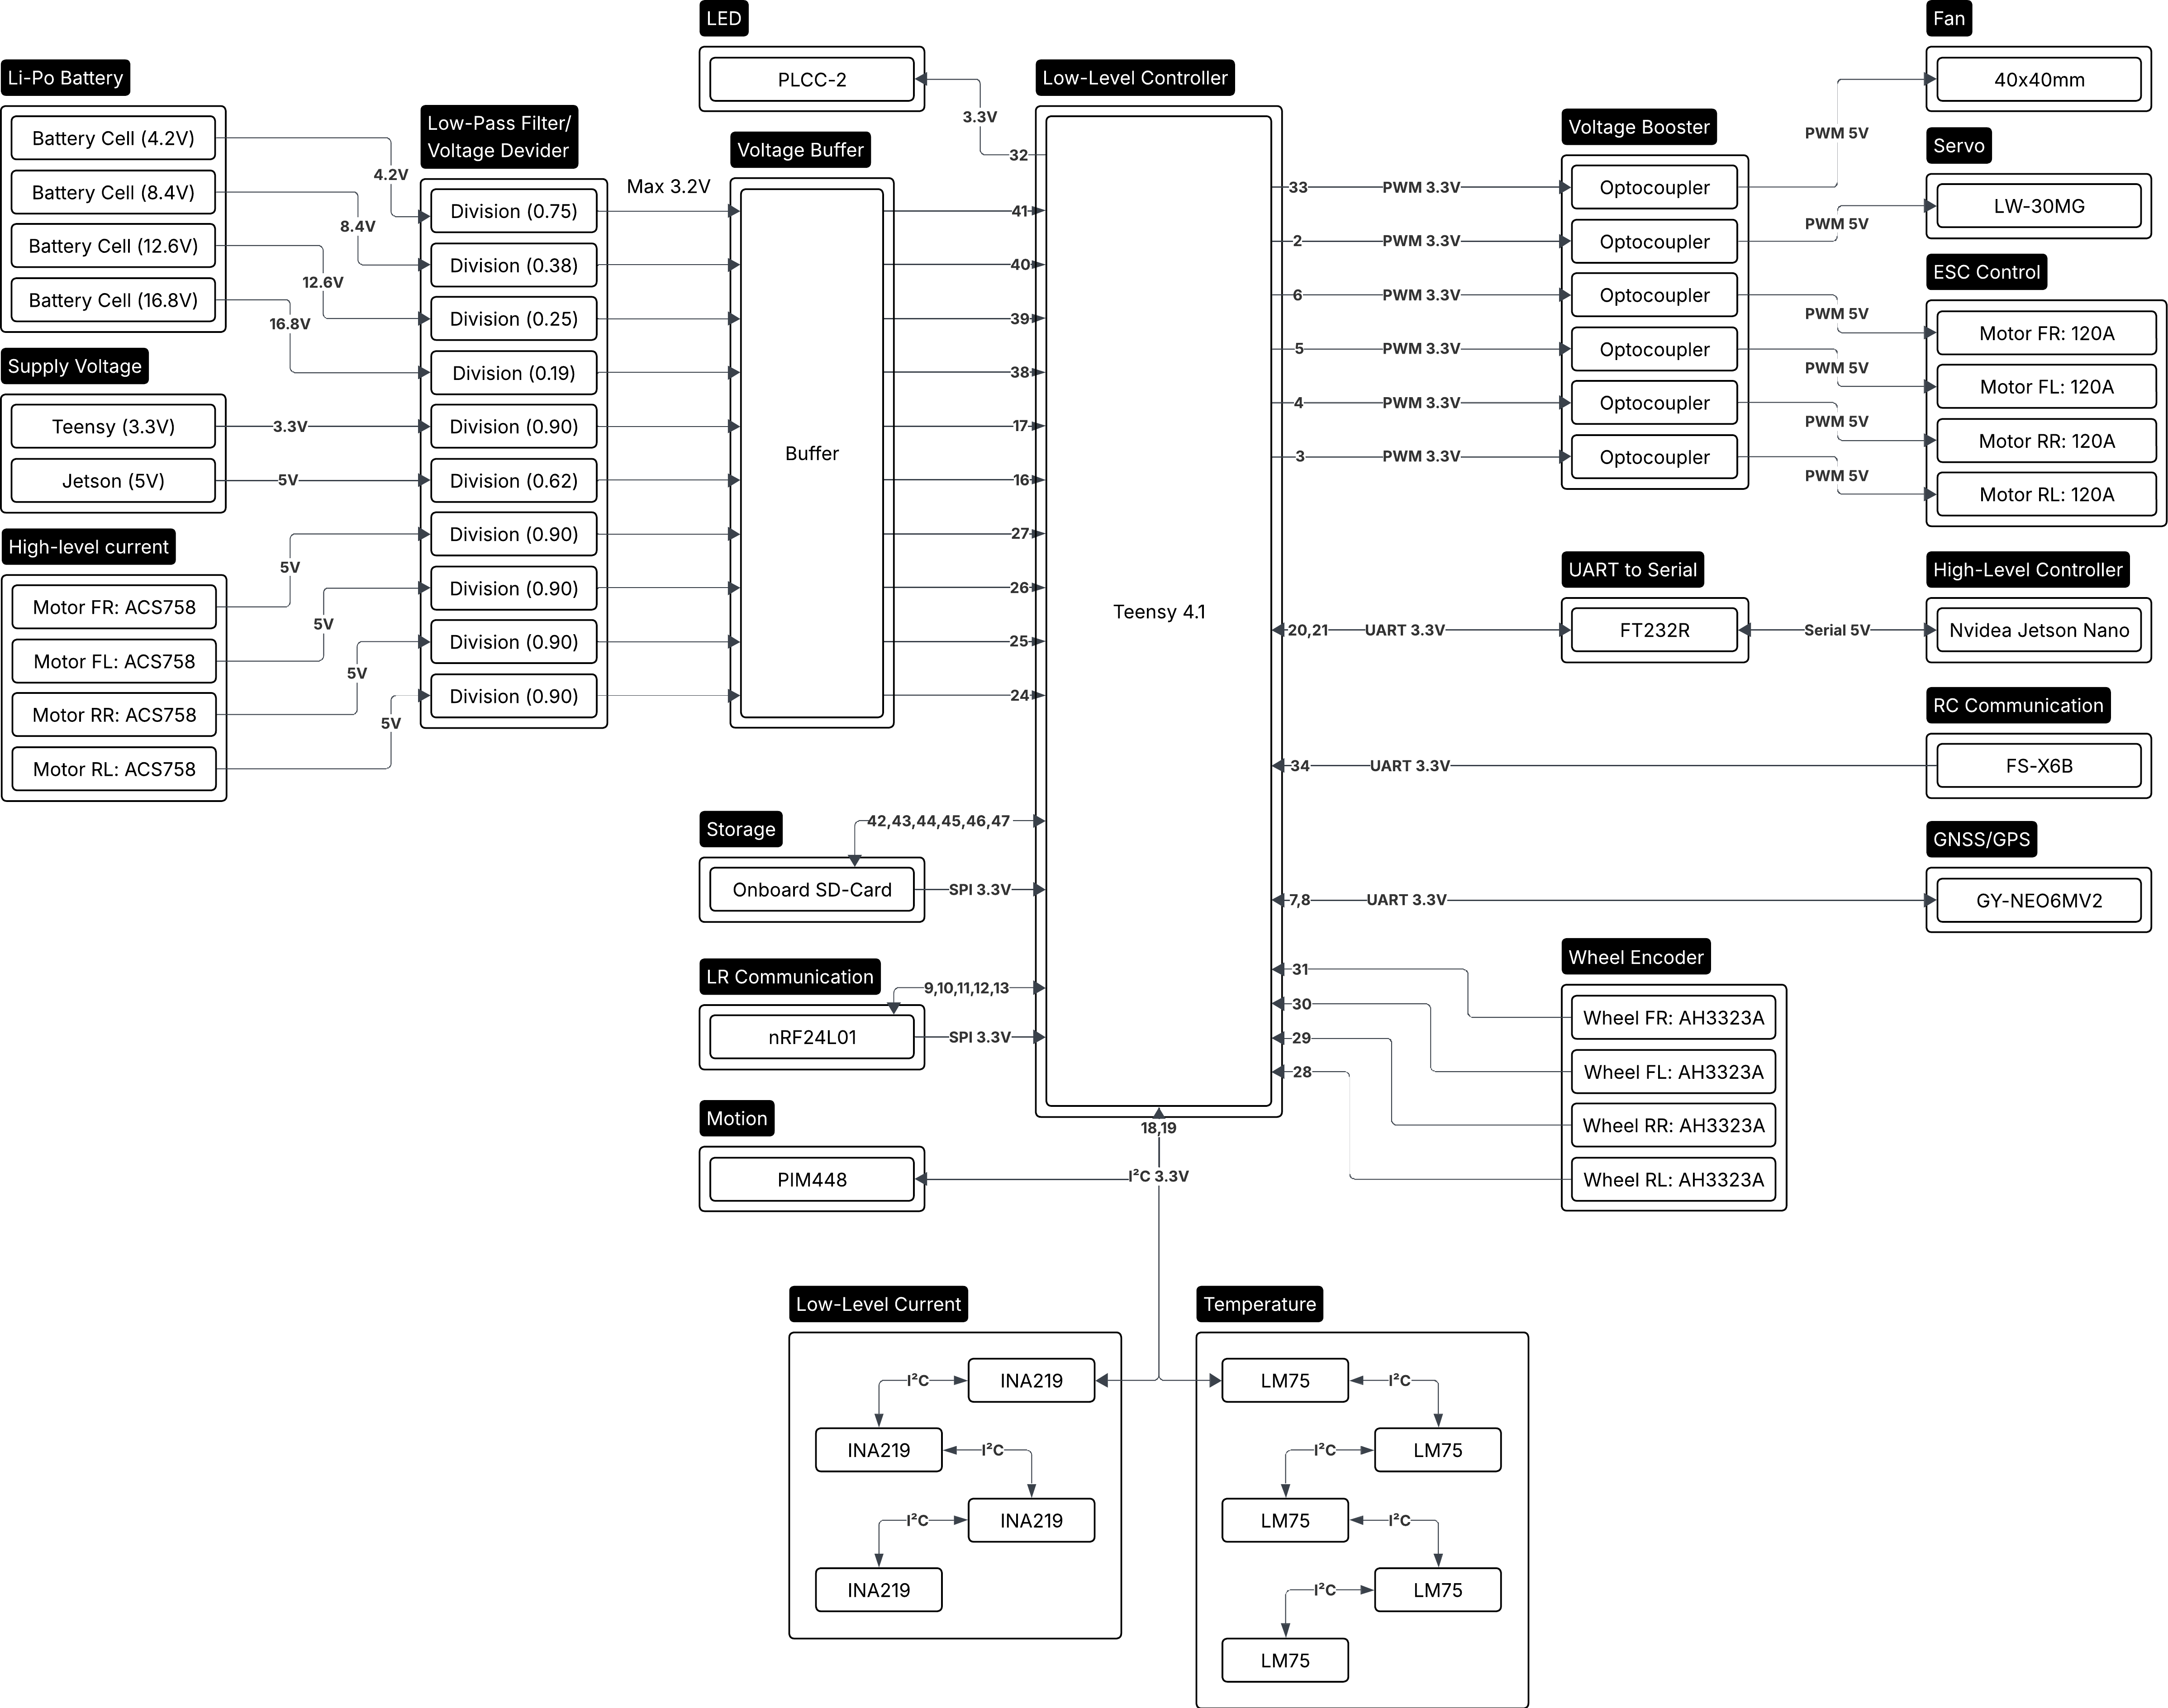
\includegraphics[width=1\textwidth, center]{images/design/lucidchart/finalized/logic_layout.png}
\end{figure}
\newpage
\section{Power design}
\RmFigWS
\begin{figure}[h!]
    \caption{TruggySense power interaction between modules}
    \centering
    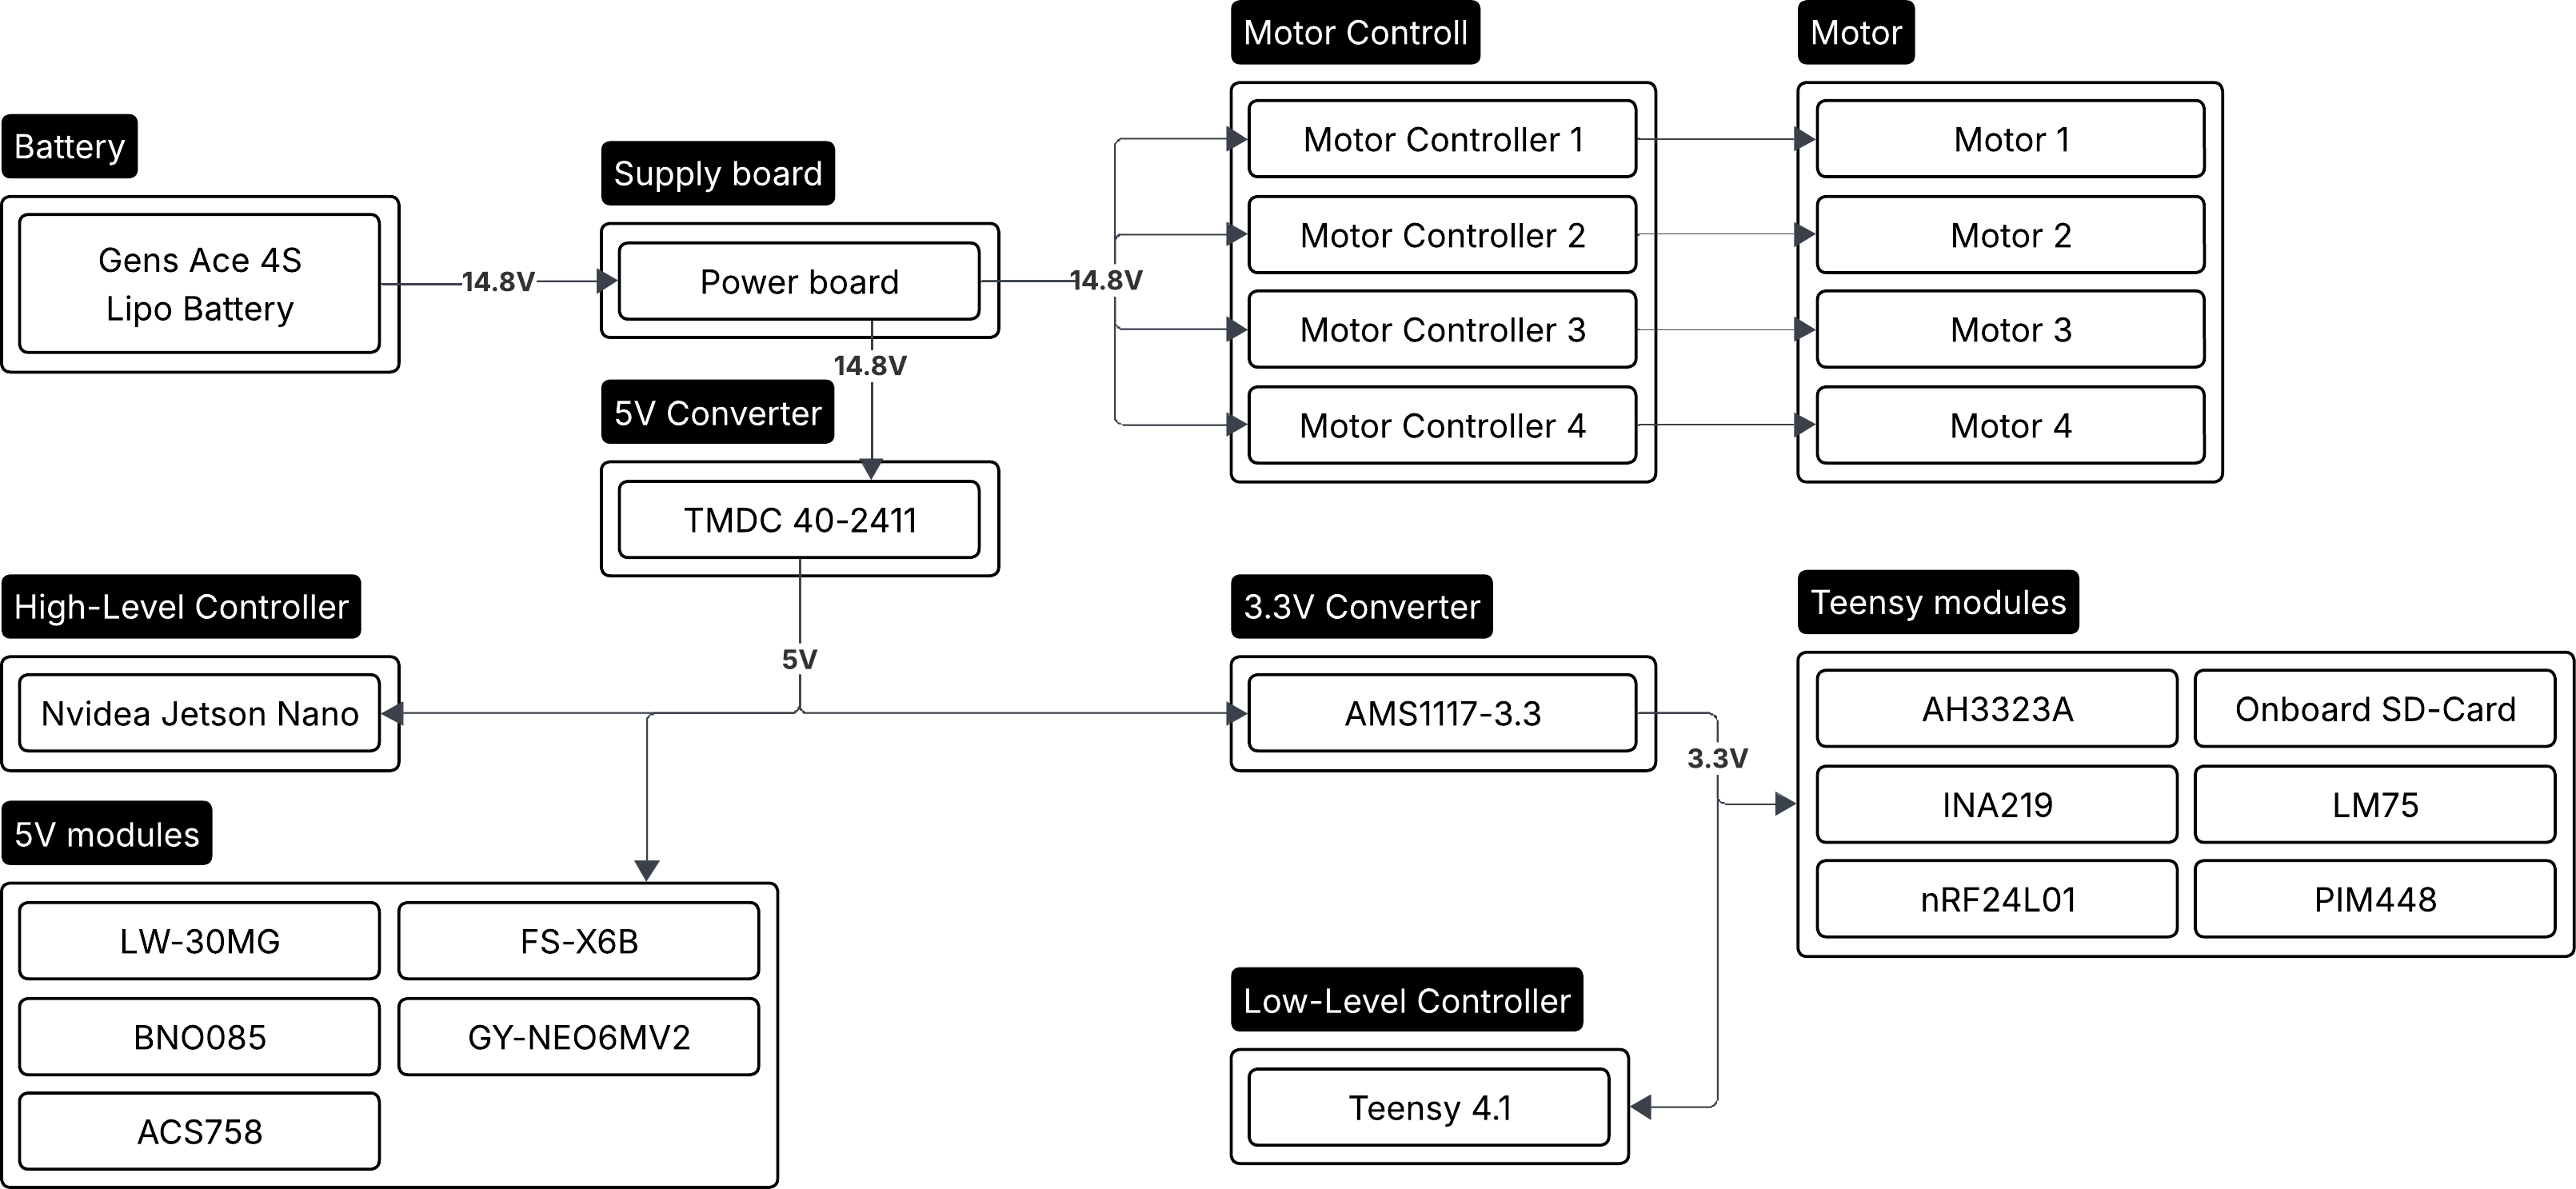
\includegraphics[width=1\textwidth, center]{images/design/lucidchart/finalized/power_layout.png}
\end{figure}
\RmFigWS
\section{KiCAD}
KiCAD 9.0 was used to design the PCBs.
The guide for this can be found in chapter~\ref{sec:kicad_guide}.

\subsection{File structure}
The file structure is similar to that of the prototype in chapter~\ref{sec:kicad_file_Structure}.
Only the modules that aren't used anymore, aren't present and the files with just a PCB sketch have been converted to footprints.
This removes the:
\RmLstWS
\begin{enumerate}[label*=\arabic*., nosep]
    \item IO-protection buffer
    \item nRF24L01
    \item PIM448
    \item LM2596 recreation
    \item Position sensor
\end{enumerate}

Leaving the following files:
\RmLstWS
\begin{enumerate}[label*=\arabic*., nosep]
    \item Logic board
    \item Power board
    \item IO-protection input
    \item IO-protection output
    \item INA219 recreation
    \item Temperature sensor
\end{enumerate}

\newpage
\subsection{Schematic}
The main difference compared to the prototype schematic, is that all the schematics in the directory are now part of the logic board schematic.
\RmFigWS
This is main the schematics for the logic board:
\begin{figure}[h!]
    \caption{TruggySense logic board electrical schematics}
    \centering
    
\includegraphics[width=1\textwidth, center]{images/design/kicad/schematic/v3/logic_board.png}
\end{figure}
\RmFigWS

The sub schematics are as follows:
\RmFigWS
\begin{figure}[h!]
    \caption{TruggySense power board electrical schematics}
    \centering
    
\includegraphics[width=0.65\textwidth, center]{images/design/kicad/schematic/v3/supply_board.png}
\end{figure}
\RmFigWS

\RmFigWS
\ImageComparison
    {TruggySense external sensor boards electrical schematics}
    {sensor_schematics}
    {{design/kicad/schematic/v3/temperature_board.png}/{Temperature sensor design (TruggySense v2)}
    /{design/kicad/schematic/v3/low_current_board.png}/{Low current sensor design (TruggySense v2)}}
\RmFigWS

\clearpage
\RmFigWS
\ImageComparison
    {TruggySense logic board communication circuits electrical schematics}
    {logic_coms_schematics}
    {{design/kicad/schematic/v3/logic_i2c.png}/{I²C circuit design (TruggySense v2)}
    /{design/kicad/schematic/v3/logic_uart.png}/{UART circuit design (TruggySense v2)},
    {design/kicad/schematic/v3/logic_spi.png}/{SPI circuit design (TruggySense v2)}
    /{design/kicad/schematic/v3/logic_various.png}/{Various communions design (TruggySense v2)},
    {design/kicad/schematic/v3/logic_pwm.png}/{PWM circuit design (TruggySense v2)}
    /{design/kicad/schematic/v3/logic_pins.png}/{Pin header design (TruggySense v2)}}
\RmFigWS

\RmFigWS
\ImageComparison
    {TruggySense IO-protection electrical schematics}
    {io_protection_schematics}
    {{design/kicad/schematic/v3/io_protection_input.png}/{Input design (TruggySense v2)}
    /{design/kicad/schematic/v3/io_protection_output.png}/{Output design (TruggySense v2)}}
\RmFigWS

\newpage
\subsection{PCB}
\subsubsection{Design rules}

\vspace{-12pt}
Click on the board setup icon 
\includegraphics[width=0.0378\textwidth]{images/design/kicad/icons/board/setup.png}.

Click open "Board Stackup"~\textgreater "Physical Stackup", and set the copper layers to 6.
The final PCBs make use of a six-layer topology:

\vspace{6pt}
\centerline{Signal | GND | 3V3 and 5V | 5V alternatives | GND | Signal}

Using this method, every component has a ground reference in close proximity.
Furthermore, both source planes have an adjacent ground plane, forming a distributed capacitor, as the FR4 layer acts as a dielectric, filtering high-frequency noise.

As for the track design rules, certain standard values were applied to the signal lines, low power lines, and high power lines (as displayed in Tab.~\ref{tab:pcb_design_rules}).
The trace widths $W$ can be determined using equation~\ref{eq:track_width}~~~\cite{Daems2023,IPC1998}.

\vspace{-18pt}
\begin{align}
    \label{eq:track_current}
    I 													  & = k \cdot \Delta T^{0.44} \cdot (W \cdot H)^{0.725} \\
	\frac{I}{k \cdot \Delta T^{0.44}} 					  & = (W \cdot H)^{0.725} \\
	(\frac{I}{k \cdot \Delta T^{0.44}})^{\frac{1}{0.725}} & = W \cdot H \\
	W 													  & = \frac{1}{H} \cdot (\frac{I}{k \cdot \Delta T^{0.44}})^{\frac{1}{0.725}}
\end{align}

\vspace{-6pt}
Since the middle layers of the PCB stack are reserved for either supply or ground planes, the traces will be on the outside, resulting in k = 0.048.
As for the temperature rise $\Delta T$ and track thickness $t$ (or $H$), standard values of 10°C and 0.035mm or 1.378 mil (1oz. copper) were used, respectively.

\vspace{-18pt}
\begin{align}
    W & = \frac{1}{1.378} \cdot \left(\frac{I}{0.048 \cdot 10^{0.44}}\right)^{\frac{1}{0.725}} \\
    \label{eq:track_width}
	  & = \frac{1}{1.378} \cdot \left(\frac{I}{0.1322}\right)^{1.379}
\end{align}

\vspace{-6pt}
This also means that a track width of $\sim$0.45m would be needed to allow a current of 200A.
Thus, a solid copper wire, with a core surface of 2.5mm², will be added to support the high current provided by the battery.

As for the vias, these should be as small as possible, while having enough surface to support the current that will pass through them.
This can be determined using equation~\ref{eq:via_current}.

\vspace{-18pt}
\begin{align}
    \label{eq:via_surface}
    A & = A_{hole} - A_{hole - copper} \\
	  & = \pi \cdot (r_{hole}^{2} - (r_{hole} - t)^{2}) \\
	  & = \pi \cdot (r_{hole}^{2} - (r_{hole}^{2} - 2 \cdot r_{hole} \cdot t + t^{2})) \\
	  & = \pi \cdot (2 \cdot r_{hole} \cdot t - t^{2}) \\
	  & = \pi \cdot t \cdot (2 \cdot r_{hole} - t) \\
	  & = \pi \cdot t \cdot (d_{hole} - t)
\end{align}

\vspace{-6pt}
Substituting it into equation~\ref{eq:track_current} gives us:

\vspace{-18pt}
\begin{align}
    d_{hole} & = t + \frac{1}{\pi \cdot t} \cdot \left(\frac{I}{k \cdot \Delta T^{0.44}}\right)^{\frac{1}{0.725}} \\
	\label{eq:via_current}
             & = 1.378 + 0.231 \cdot \left(\frac{I}{0.1322}\right)^{1.3793}
\end{align}

\vspace{-6pt}
The pad diameter will be twice the hole diameter, to ensure a good connection between the via and layers.

Finally, for spacing, a 0.13mm clearance should suffice for the signal and low power lines~~\cite{Daems2023}.
As for the high power lines, a clearance of at least 1mm is used to make sure that the ground plane of the logic board and supply board can never connect to each other.

\begin{table*}[!h]
	\centering
	\caption{PCB Design Rules}
	\begin{tabular}{lcccccccc}
		\toprule
			Line type & \multicolumn{2}{c}{Power}   						& \multicolumn{2}{c}{Traces} 					     & \multicolumn{3}{c}{Vias}   						                             & Spacing \\
					  &	\scriptsize{Voltage (V)} & \scriptsize{Current (A)} & \scriptsize{Width (mil)} & \scriptsize{Width (mm)} & \scriptsize{Hole (mil)}  & \scriptsize{Hole (mm)} & \scriptsize{Diameter (mm)} & \scriptsize{Clearance (mm)} \\
		\cmidrule(lr){2-3}\cmidrule(lr){4-5}\cmidrule(lr){6-8}\cmidrule(lr){9-9}
			\small{Signal}     & \textless 5.1  & \textless 0.1 & 0.494 & 0.0125 & 1.535 & 0.039 & 0.078 & 0.13 \\
			\small{Low power}  & \textless 5.1  & \textless 2   & 30.76 & 0.7814 & 11.17 & 0.284 & 0.568 & 0.26 \\
			\small{High power} & \textless 16.8 & \textless 200 & 17647 & 448.22 & 5619  & 142.7 & 285.4 & 1.3  \\
		\bottomrule
	\end{tabular}
	\label{tab:pcb_design_rules}
\end{table*}

Click open "Design Rules"~\textgreater "Pre-defined Sizes", and add the values to the table.

Click open "Design Rules"~\textgreater "Net Classes", and change the clearance of the default net class, then apply the logic for the High power lines.

\vspace{-6pt}
\subsubsection{Design}
Since all schematics are part of the same project, the same goes for the PCB.
\RmFigWS
\begin{figure}[h!]
    \caption{TruggySense logic board PCB-design}
    \centering
    \includegraphics[width=1\textwidth, center]{images/design/kicad/board/v3/PCB.png}
\end{figure}
\RmFigWS

The PCB makes use of four layers (explanations can be found \href{https://www.allpcb.com/blog/pcb-design/how-to-design-a-multi-layer-navigation-pcb-for-complex-systems.html}{here}):
\RmLstWS
\begin{enumerate}[nosep]
    \item Primary signal layer
    \item Ground plane
    \item Primary supply plane (both 3V3 and 5V)
    \item Secondary supply plane (variations of the 5V rail)
    \item Ground plane
    \item Secondary signal layer
\end{enumerate}
\newpage
\section{Assembly}
An assembly of the finalized design wasn't possible within the time scope of this project.
Thus a 3D-render will be provided:
\RmFigWS
\begin{figure}[h!]
	\centering
	\subfloat[PCB top view]{
		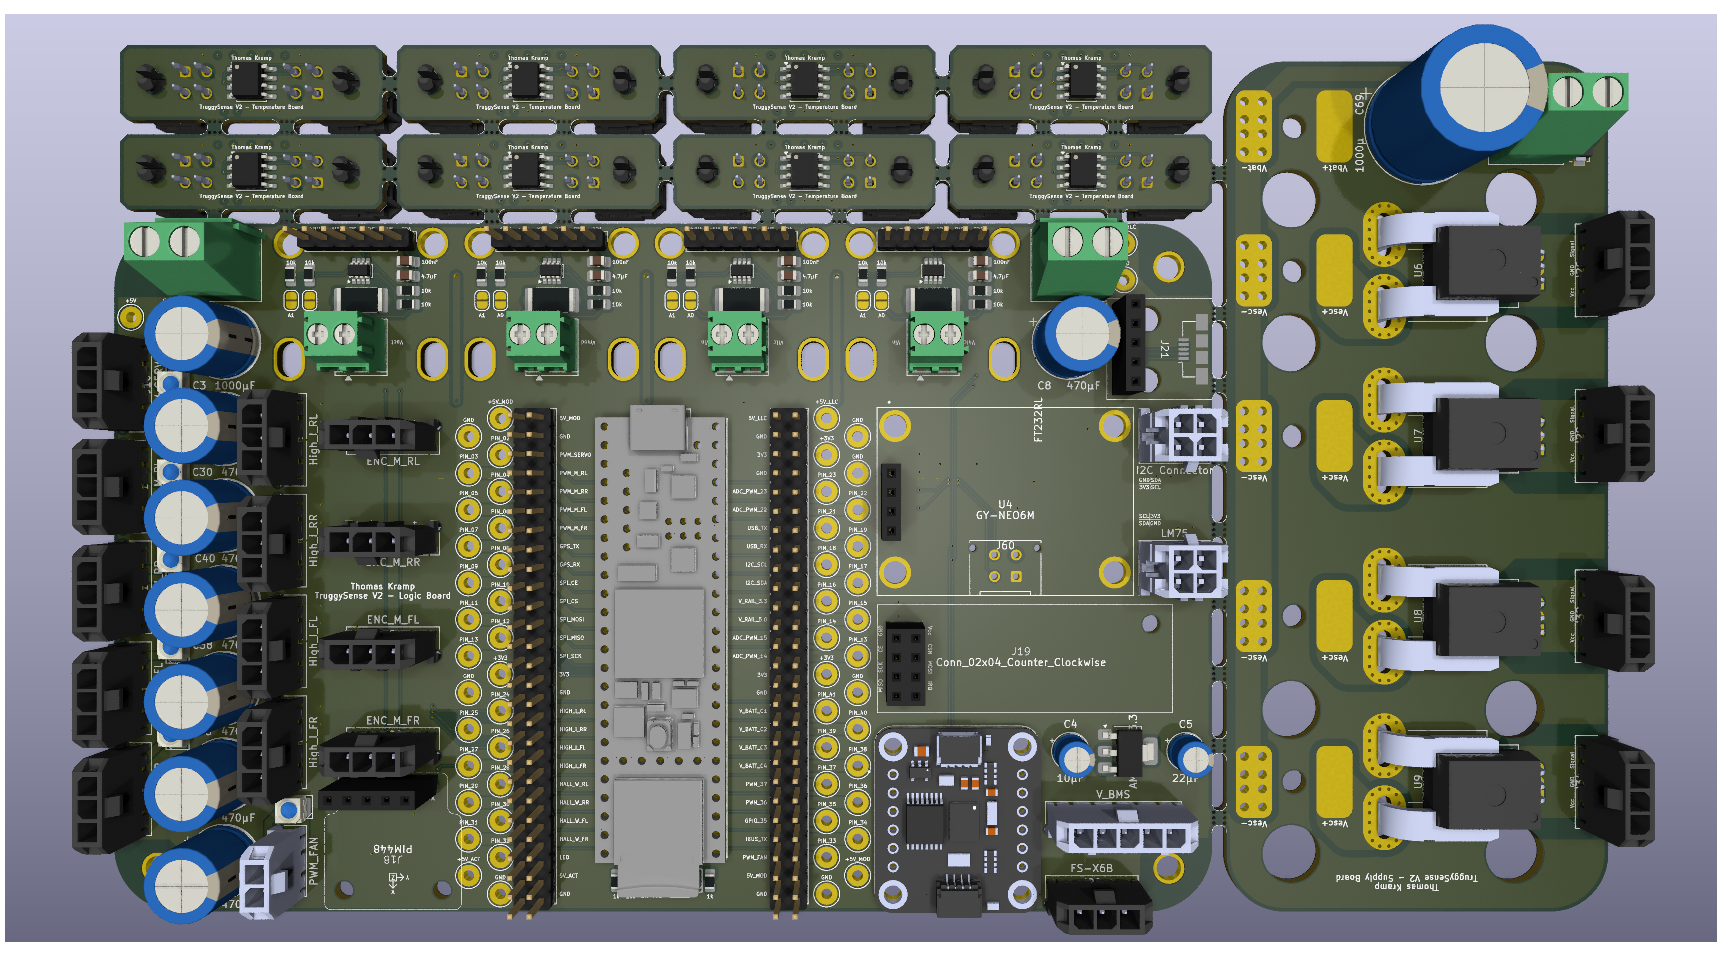
\includegraphics[width=1\textwidth, center]{images/design/assembly/v3/pcb_top.png}
	} \hfil
	\subfloat[PCB bottom view]{
		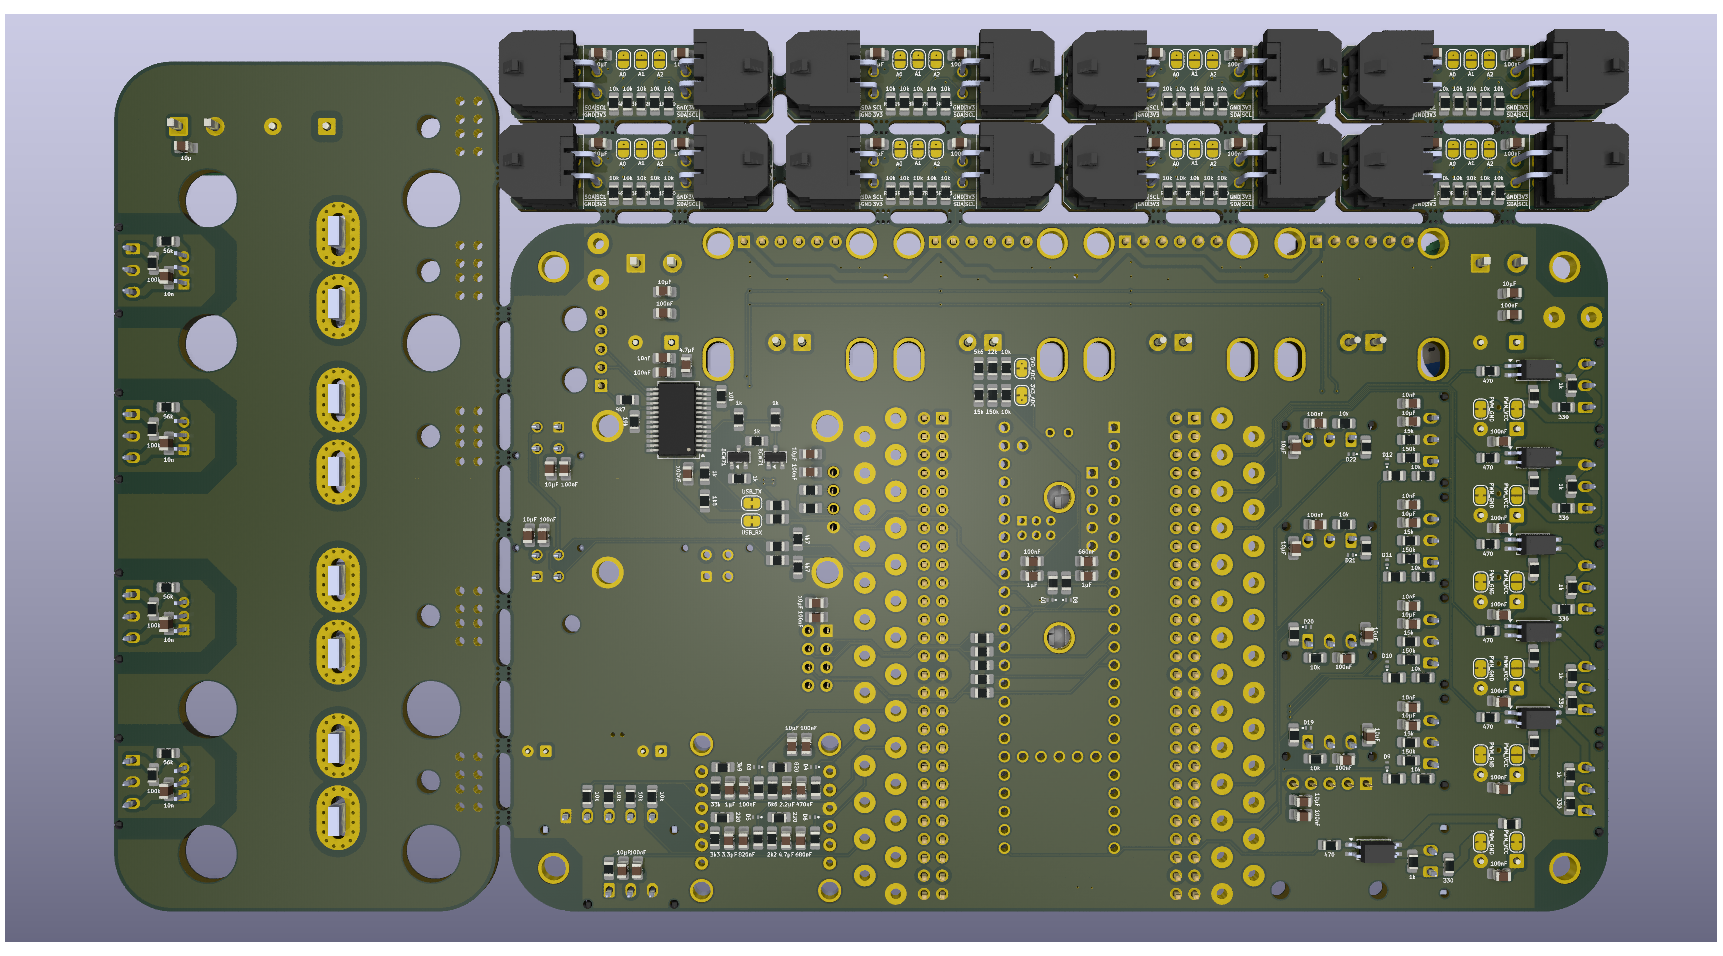
\includegraphics[width=1\textwidth, center]{images/design/assembly/v3/pcb_bottom.png}
	}
	\caption{3D-render of the TruggySense V2 finalized PCB-design}
\end{figure}
\RmFigWS

\subsection{BOM}
The KiCAD BOM extension can be installed using the guide in section~\ref{sec:kicad_bom}

\href{../../cad/KiCAD/v3/board_logic/bom/ibom.html}{Click here to see the interactive BOM.}
\Needspace{10\baselineskip}     % Set table not prematurely overflow to next page
\begin{table}[h!]
    \centering
    \caption{Bill of materials of the TruggySense v2}
    \begin{adjustbox}{max width=\textwidth, max height=1\textheight}
        \begin{tabular}{l r c c}
            \toprule
                \textbf{Component} & \textbf{Value} & \textbf{Qty} & \textbf{Footprint} \\
            \midrule
                \csvreader[
                    head to column names,
                    late after line=\\,
                ]{./databases/design/bom/finalized.csv}{}{
                    \href{\PurchaseLink}{\Component} & 
                    \href{\PurchaseLink}{\Value} &
                    \href{\PurchaseLink}{\Qty} & 
                    \Footprint
                }
            \bottomrule
        \end{tabular}
    \end{adjustbox}
    \label{tab:bill_of_materials}
\end{table}
\section{FreeCAD}
KiCAD 9.0 was used to design the PCBs.
The guide for this can be found in chapter~\ref{sec:freecad_guide}.
\subsection{Designs recommendations}
A new setup for the full assembly couldn't be made due to time constrains.
These are some recommendations if you want to build a full assembly for the finalized PCB:
\begin{itemize}
    \item Create casings for the Logic-, Supply- and Temperature Sensor board.
    \item Increase the sizes of the holes in the HLC-casing, that mount the case to the base plate.
    \item Mount the antenna module to the inside of the lid.
    \item Add holes that allow access to the GPIO pins of the HLC.
    \item Rotate both the TMDC holder and HLC such that the IO of the HLC is pointed towards the left side (battery side) of the vehicle.
    \item Create a TMDC 40-2411 holder and put it at an angle such that there is a hole between it and the HLC case.
          This will allow that hole, to act as a cable management clip.
    \item Recreate the rear mounts, such that the screws are clear of the mounting protrusions of the lid.
    \item Widen the base plate to be as wide as the bottom chassis.
    \item Make it so that the base plate can be placed (or be removed) more easily from the chassis, enlarging the cut-outs for the mounting protrusions of the lid.
    \item Bring the logic- and supply-boards more to the center of the base plate.
    \item Redo all the mounting holes on the base plate.
\end{itemize}

Note that both the casings for the \textbf{\href{https://www.printables.com/model/548510-gps-gy-gps6mv2-module-case-neo-6m}{GPS-module}} and the \textbf{\href{https://www.treatstock.com/blog/3d-printed-cases-for-nvidia-jetson-nano}{HLC}}, were taken from external sources.
Click on the bold-face text to open them.
\section{Metalcut}
MetalCut was used to prepare the laser cut.
The guide for this can be found in chapter~\ref{sec:metalcut_guide}.

I recommend to use a 4mm thick Acrylic/PMMA plate instead of the 6mm.
If you do change that means that \textbf{these values aren't correct anymore}:
\RmLstWS
\begin{itemize}
    \item Power 85\%
    \item Speed 12mm/s
\end{itemize}
\RmLstWS
Make sure to change them.

\chapter{Software}                  % ---------------------- Software ----------------------
\section{Install ArduinoIDE}
Don't worry we won't use the ArduinoIDE, it is just a requirement to run PlatformIO.
\section{Install PlatformIO}
Global install of platformIO (on Linux):
\begin{lstlisting}[style=cmd]
    pip3 install -U platformio
\end{lstlisting}

Check the installation:
\begin{lstlisting}[style=cmd]
    pio --version
\end{lstlisting}

Install via VS code.
On the left side choose "Plugins" and install:
\begin{enumerate}[nosep]
    \item C/C++ Extension Pack
    \item PlatformIO IDE
\end{enumerate}

Enable "pio" command on debian 12
\begin{lstlisting}[style=cmd]
    nano ~/.bashrc
\end{lstlisting}

At the bottom of the file paste this:
\begin{lstlisting}[style=script]
    export PATH="$HOME/.platformio/penv/bin:$PATH"
\end{lstlisting}

Save and close the file and reload:
\begin{lstlisting}[style=cmd]
    source ~/.bashrc
\end{lstlisting}

Check the installation:
\begin{lstlisting}[style=cmd]
    pio --version
\end{lstlisting}
\newpage
\section{Module testing}
\subsection{Teensy 4.1}
Plug in the teensy and run:
\begin{lstlisting}[style=cmd]
    pio device list
\end{lstlisting}

The output should look something like:
\begin{lstlisting}[style=script]
    /dev/ttyACM0
    ------------
    Hardware ID: USB VID:PID=16C0:0483 SER=15284150 LOCATION=1-8:1.0
    Description: USB Serial
\end{lstlisting}

For a more detailed output, run:
\begin{lstlisting}[style=cmd]
    pio device monitor
\end{lstlisting}

The output should look something like:
\begin{lstlisting}[style=script]
    --- Terminal on /dev/ttyACM0 | 9600 8-N-1
    --- Available filters and text transformations: debug, default, direct, hexlify, log2file, nocontrol, printable, send_on_enter, time
    --- More details at https://bit.ly/pio-monitor-filters
    --- Quit: Ctrl+C | Menu: Ctrl+T | Help: Ctrl+T followed by Ctrl+H
\end{lstlisting}

If the command gives a "permission denied" use:
\begin{lstlisting}[style=cmd]
    sudo chmod a+rw /dev/ttyACM0
\end{lstlisting}

Find the board:
\begin{lstlisting}[style=cmd]
    pio boards | grep Teensy
\end{lstlisting}

The output should include:
\begin{lstlisting}[style=script]
    teensy41   IMXRT1062    600MHz       7.75MB   512KB     Teensy 4.1
\end{lstlisting}

Create a directory for the project and go to it:
\begin{lstlisting}[style=cmd]
    cd TruggySense/code/module_tests/Teensy41/
\end{lstlisting}

Create a udev rule:
\begin{lstlisting}[style=cmd]
    sudo nano /etc/udev/rules.d/49-teensy.rules
\end{lstlisting}

Add the following to the file:
\begin{lstlisting}[style=script]
    SUBSYSTEM=="usb", ATTR{idVendor}=="16c0", MODE:="0666"
    KERNEL=="hidraw*", ATTRS{idVendor}=="16c0", MODE:="0666"
\end{lstlisting}

Save and close the file.

Reload udev:
\begin{lstlisting}[style=cmd]
    sudo udevadm control --reload-rules
    sudo udevadm trigger
\end{lstlisting}

Create a project:
\begin{lstlisting}[style=cmd]
    pio project init --board teensy41
\end{lstlisting}

A "platformio.ini" file should have been created, containing:
\begin{lstlisting}[style=platformio]
    [env:teensy41]
    platform = teensy
    board = teensy41
    framework = arduino
\end{lstlisting}

There should also be a "src" folder.
Create a new file called "main.cpp" inside that folder.

Paste the default Arduino code:
\begin{lstlisting}[style=platformio]
    #include "Arduino.h"

    #ifndef LED_BUILTIN
    #define LED_BUILTIN 13
    #endif

    void setup() {
      // initialize LED digital pin as an output.
      pinMode(LED_BUILTIN, OUTPUT);
    }

    void loop() {
      // turn the LED on (HIGH is the voltage level)
      digitalWrite(LED_BUILTIN, HIGH);

      // wait for a second
      delay(1000);

      // turn the LED off by making the voltage LOW
      digitalWrite(LED_BUILTIN, LOW);

      // wait for a second
      delay(1000);
    }
\end{lstlisting}

Run the code using:
\begin{lstlisting}[style=cmd]
    pio run -t upload
\end{lstlisting}

When doing so this window will pop up:
\RmFigWS
\begin{figure}[h!]
    \centering
    \caption{Teensy pop-up window}
    \begin{subfigure}{\DualColumnWidth\textwidth}
        \centering
        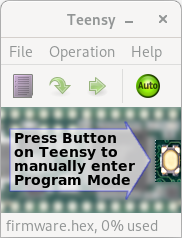
\includegraphics[width=10em]{./images/programming/teensy_upload_halted.png}
        \caption{Upload halted}
        \label{fig:teensy_upload_halted}
    \end{subfigure}
    \begin{subfigure}{\DualColumnWidth\textwidth}
        \centering
        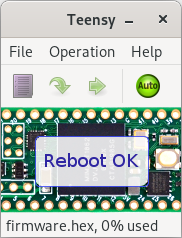
\includegraphics[width=10em]{./images/programming/teensy_upload_succes.png}
        \caption{Upload success}
    \end{subfigure}
    \label{fig:teensy_pop_up}
\end{figure}
\RmFigWS

Sometimes it will automatically upload, other times it requires you to press the reset button.
Do not press it before and while uploading it, only when the pop-up window requires it.
\subsection{UART communication}
\begin{lstlisting}[style=cmd]
# Plug in the teensy and run:
    pio device list

# If the command gives a "permission denied" use:
    sudo chmod a+rw /dev/ttyACM0

# Activate the UART communication:
    pio device monitor --port /dev/ttyACM0 --baud 115200
\end{lstlisting}
\RmLstWS\RmFigWS
\section{ROS2 integration}
\subsection{Install Docker}
These are the steps needed to install docker on debian 13:
\begin{lstlisting}[style=cmd]
# Install docker:
    sudo apt update && sudo apt install docker.io docker-compose

# Allow docker usage without sudo command:
    sudo groupadd docker && sudo usermod -aG docker $USER
\end{lstlisting}
\RmFigWS
\subsection{Setup the Teensy}
\href{Uhttps://micro.ros.org/docs/tutorials/core/teensy_with_arduino/RL}{This is the guide that was used as a basis for setting up micro-ROS on the Teensy module.}

First of all create a teensy project using PlatformIO.

A "platformio.ini" file should have been created.
Add the following:
\begin{lstlisting}[style=platformio]
    [env:teensy41]
    platform = teensy
    board = teensy41
    framework = arduino
    monitor_speed = 115200
    upload_protocol = teensy-cli
    board_microros_distro = humble
    board_microros_transport = serial
    lib_deps = https://github.com/micro-ROS/micro_ros_platformio
\end{lstlisting}

There should also be a "src" folder.
Create a new file called "main.cpp" inside that folder.
Paste the default Arduino code:
\begin{lstlisting}[style=platformio]
    #include <Arduino.h>                  // Must include this first for Arduino functions
    #include <micro_ros_platformio.h>
    #include <rcl/rcl.h>
    #include <rclc/rclc.h>
    #include <std_msgs/msg/int32.h>

    #ifndef LED_BUILTIN
    #define LED_BUILTIN 13
    #endif

    // micro-ROS objects
    rcl_publisher_t publisher;
    rcl_node_t node;
    rclc_support_t support;
    rcl_allocator_t allocator;
    std_msgs__msg__Int32 msg;

    bool connected = false;

    void setup() {
        // Initialize Serial and LED
        Serial.begin(115200);
        delay(2000);
        pinMode(LED_BUILTIN, OUTPUT);

        // Set up micro-ROS transport
        set_microros_serial_transports(Serial);

        allocator = rcl_get_default_allocator();

        // Attempt to connect
        while (!connected) {
            Serial.println("Trying to connect to micro-ROS agent...");
            rcl_ret_t ret;

            // Initialize support
            ret = rclc_support_init(&support, 0, NULL, &allocator);
            if (ret != RCL_RET_OK) {
                Serial.println("Failed to init support, retrying...");
                delay(1000);
                continue;
            }

            // Initialize node
            ret = rclc_node_init_default(&node, "teensy_node", "", &support);
            if (ret != RCL_RET_OK) {
                Serial.println("Failed to init node, retrying...");
                rclc_support_fini(&support);
                delay(1000);
                continue;
            }

            // Initialize publisher
            ret = rclc_publisher_init_default(
                &publisher,
                &node,
                ROSIDL_GET_MSG_TYPE_SUPPORT(std_msgs, msg, Int32),
                "teensy_counter"
            );
            if (ret != RCL_RET_OK) {
                Serial.println("Failed to init publisher, retrying...");
                rcl_node_fini(&node);
                rclc_support_fini(&support);
                delay(1000);
                continue;
            }

            // Successfully connected
            connected = true;
            Serial.println("Connected to micro-ROS agent!");
        }

        msg.data = 0;
    }

    void loop() {
        // Blink LED
        digitalWrite(LED_BUILTIN, HIGH);
        delay(500);
        digitalWrite(LED_BUILTIN, LOW);
        delay(500);

        // Publish micro-ROS message
        msg.data++;
        rcl_publish(&publisher, &msg, NULL);
    }
\end{lstlisting}
\newpage
In the command promt type:
\begin{lstlisting}[style=cmd]
    nano Dockerfile.pio
\end{lstlisting}

\begin{lstlisting}[style=script]
    # 1) Get image
    FROM ros:humble

    # 2) Change the shell instruction type
    SHELL ["/bin/bash", "-c"]

    # 3) Get variables
    ARG GIT_USER_NAME
    ARG GIT_USER_EMAIL

    # 4) Install dependencies
    RUN apt update && apt install -y \
        build-essential \
        git \
        libasio-dev \
        python3-colcon-common-extensions \
        python3-pip \
        python3-rosdep \
        python3-venv \
        && rm -rf /var/lib/apt/lists/*

    # 5) Fix git issues
    RUN git config --global pull.rebase false && \
        git config --global --add safe.directory /workspace && \
        git config --global user.name "${GIT_USER_NAME}" && \
        git config --global user.email "${GIT_USER_EMAIL}" && \
        git config --global --add safe.directory /workspace/.pio/libdeps/teensy41/micro_ros_platformio/build/dev/src/ament_cmake

    # 6) Setup the virtual environment for PlatformIO
    RUN python3 -m venv ~/.platformio/penv && \
        ~/.platformio/penv/bin/python -m pip install --upgrade pip && \
        ~/.platformio/penv/bin/python -m pip install -U platformio catkin_pkg empy==3.3.4 lark-parser pyyaml
        
    # 7) Update the system
    RUN apt update -y && apt upgrade -y && apt autoremove -y

    # 8) Open the terminal inside the container
    CMD ["/bin/bash"]
\end{lstlisting}

\begin{lstlisting}[style=cmd]
    nano docker-compose.yaml
\end{lstlisting}

\begin{lstlisting}[style=script]
version: "3.8"

services:
  microros:
    build:
      context: .
      dockerfile: Dockerfile.pio
      args:
        GIT_USER_NAME: "${GIT_USER_NAME}"
        GIT_USER_EMAIL: "${GIT_USER_EMAIL}"

    container_name: microros-pio
    privileged: true
    stdin_open: true
    tty: true

    volumes:
      - ${HOST_WORKSPACE_PATH}/TruggySense/code/protocol_tests/ROS2:/workspace
      - /dev:/dev

    environment:
      - ROS_DOMAIN_ID=0

    command: /bin/bash
\end{lstlisting}

\begin{lstlisting}[style=cmd]
    nano .env
\end{lstlisting}

\begin{lstlisting}[style=script]
GIT_USER_NAME=<Git username>
GIT_USER_EMAIL=<Git mail>

# Only the BASE path here!
HOST_WORKSPACE_PATH=<Path to TruggySense directory>
\end{lstlisting}

\begin{lstlisting}[style=cmd]
    docker-compose up -d
    docker exec -it microros-pio /bin/bash
\end{lstlisting}

Or run the Dockerfile manually:
\begin{lstlisting}[style=cmd]
    docker image prune -a
    sudo rm -rf ~/<PATH>/TruggySense/code/protocol_tests/ROS2/.pio
    rm -rf /workspace/pio
    docker build -t microros-pio -f Dockerfile.pio .
    docker run -it --rm --net=host -v /dev:/dev --privileged -v ~/<PATH>/TruggySense/code/protocol_tests/ROS2:/workspace microros-pio
    # -it           --> i = interactive & t = allocates terminal --> Use the container shell
    # --net=host    --> Uses the host's network instead of the internal docker network
    # -v dev/dev    --> Mounts the host's connected devices to the docker container
    # --privileged  --> Gives the container full access to the host's system (needed for hardware) 
\end{lstlisting}

To run the code:
\begin{lstlisting}[style=cmd]
    cd /workspace
    source ~/.platformio/penv/bin/activate
    pio run -t upload -e teensy41
    pio device monitor -b 115200
\end{lstlisting}
\subsection{Setup the Jetson}
\href{https://developer.nvidia.com/embedded/learn/get-started-jetson-nano-devkit}{Click here to follow a guide to setup the jetson.}

If using the micro-usb port for power, make sure to disconnect jumper J48. You can place this jumper over the 5V pins for safekeeping.

\begin{lstlisting}[style=cmd]
    sudo apt update && sudo apt -y upgrade && sudo apt -y autoremove
    sudo apt install docker.io dockercompose
    nano Dockerfile
\end{lstlisting}

\begin{lstlisting}[style=script]
    # 1) Get image
    FROM ros:humble

    # 2) Change the shell instruction type
    SHELL ["/bin/bash", "-c"]

    # 3) Get variables
    ARG GIT_USER_NAME
    ARG GIT_USER_EMAIL

    # 4) Install dependencies
    RUN apt update && apt install -y \
        build-essential \
        git \
        libasio-dev \
        python3-colcon-common-extensions \
        python3-pip \
        python3-rosdep \
        python3-venv \
        && rm -rf /var/lib/apt/lists/*
        
    # 5) Fix git issues
    RUN git config --global pull.rebase false && \
        git config --global --add safe.directory /workspace && \
        git config --global user.name "${GIT_USER_NAME}" && \
        git config --global user.email "${GIT_USER_EMAIL}" && \
        git config --global --add safe.directory /workspace/.pio/libdeps/teensy41/micro_ros_platformio/build/dev/src/ament_cmake
        
    # 6) Update the system
    RUN apt update -y && apt upgrade -y && apt autoremove -y

    # 7) Open the terminal inside the container
    CMD ["/bin/bash"]
\end{lstlisting}

\begin{lstlisting}[style=cmd]
    sudo apt update
    sudo apt Upgrade
    sudo apt autoremove

    sudo apt install docker.io dockercompose
    nano Dockerfile
\end{lstlisting}

\begin{lstlisting}[style=cmd]
    docker image prune -a
    docker build -t ros-transceiver -f Dockerfile .
    docker run -it --rm --net=host -v /dev:/dev --privileged -v ~/<PATH>/TruggySense/code/protocol_tests/ROS2:/workspace ros-transceiver
\end{lstlisting}

\begin{lstlisting}[style=cmd]
# Install the micro-ros interpreter on the host machine
# - Create workspace for the micro_ros_setup of Humble
    mkdir -p ~/agent_ws/src
    cd ~/agent_ws/src
    git clone -b humble https://github.com/micro-ROS/micro-ros-build.git micro_ros_setup

# - Build micro-ros environment
    cd ~/agent_ws
    source /opt/ros/humble/setup.bash
    rosdep fix-permissions
    rosdep update
    rosdep install --from-paths src --ignore-src -y
    colcon build

# - Build the agent
    source install/local_setup.bash
    ros2 run micro_ros_setup create_agent_ws.sh
    ros2 run micro_ros_setup build_agent.sh

# Start ROS host container:
    cd ~/agent_ws
    source install/local_setup.bash
    ros2 run micro_ros_agent micro_ros_agent serial --dev /dev/ttyACM0 -b 115200

# View ROS host messages:
    source /opt/ros/humble/setup.bash
    ros2 topic list
    ros2 topic echo /teensy_counter
\end{lstlisting}

% https://github.com/micro-ROS/micro_ros_platformio
% pio pkg install # Install dependencies
%
% pio run --target upload # Flash the firmware

% After library changes:
% pio run --target clean_microros  # Clean library

% Serial micro-ROS Docker Agent
% docker run -it --rm -v /dev:/dev -v /dev/shm:/dev/shm --privileged --net=host microros/micro-ros-agent:$ROS_DISTRO serial --dev [YOUR BOARD PORT] -v6

\chapter{Testing \& validation}     % ---------------------- Testing & validation  ----------------------
\section{Install Matlab}
The installation file can be found using \href{https://nl.mathworks.com/downloads/}{this link}.

The installation for Linux (Debian and Ubuntu) can be done using the following commands:
\begin{lstlisting}[style=cmd]
# Unzip the file:
    unzip matlab_R2026a_Linux.zip -d ./matlab_R2026a_Linux && cd ./matlab_R2026a_Linux

# Install KiCad:
    sudo apt update 
    sudo xhost +SI:localuser:root
    sudo -H ./install
    sudo xhost -SI:localuser:root

# Open Matlab:
     /usr/local/MATLAB/R20XXy/bin/matlab
\end{lstlisting}
\RmLstWS
\subsection{Install plugins}
Once Matlab is running go to the "Home"-tab and click on the "Add-Ons \textgreater~Explore Add-Ons"-button to open the add-on explorer.
Then install the following extensions:
\RmLstWS
\begin{itemize}
    \item Curve Fitting Toolbox
    \item Antenna Toolbox
    \item Statistics and Machine Learning Toolbox
    \item Phased Array System Toolbox
    \item Image Processing Toolbox
\end{itemize}
\RmLstWS

\subsection{File structure}
The test files can be cound under "code/matlab/paper_Scripts".
It makes use of .json files to read in the data.
\newpage
\section{Experiments}
\subsection{Setup}
As demonstrated by the TruggySense V1, the system is designed to verify and validate the ADAS under various off-road conditions.
To prove this, four experiments were performed on a predefined path (Fig.~\ref{fig:track}): (1) Slow driving, (2) Fast driving, (3) Failure detection, and (4) Crash detection.
Experiments (1) and (2) have proven to sense the characteristics of the environment, using data pertaining to the condition of the vehicle, while experiments (3) and (4) were, in turn, able to demonstrate that the DAQ could sense malfunctions.

\begin{figure}[!h]
	\centering
	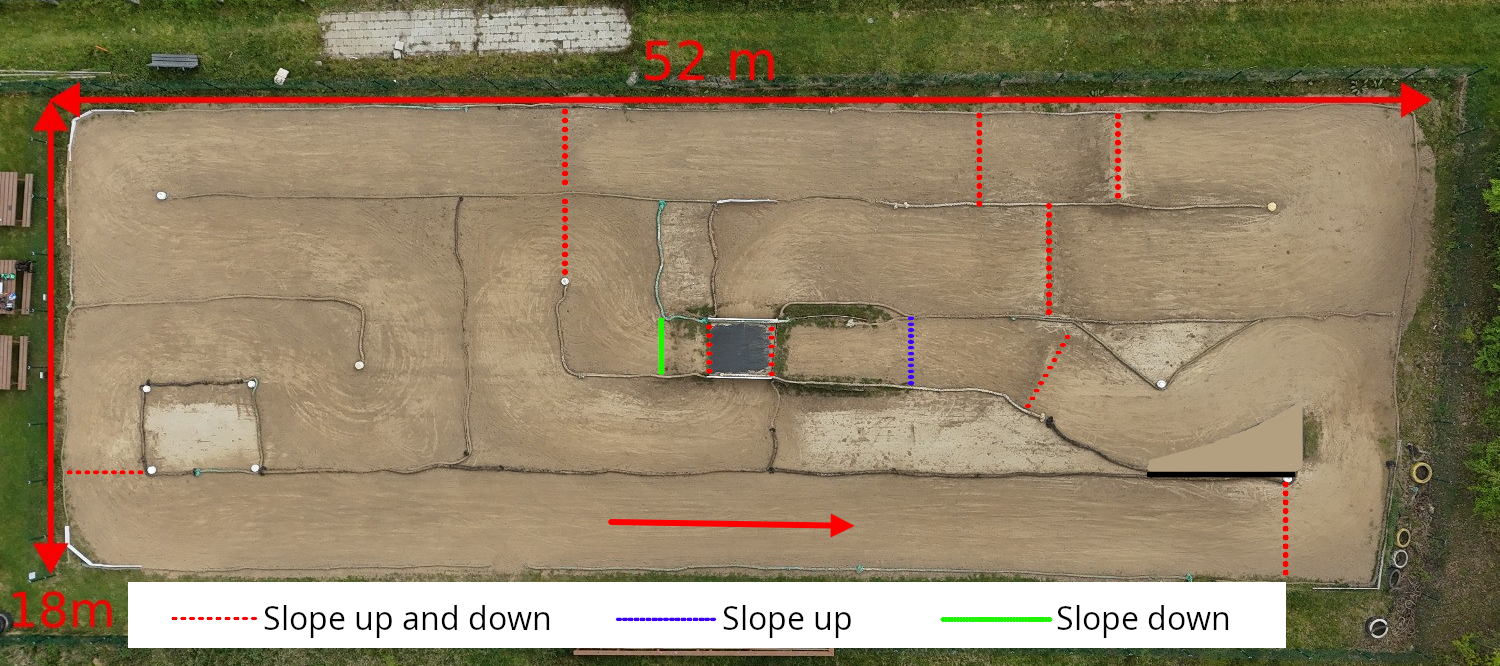
\includegraphics[width=0.5\textwidth]{images/experiments/track_indication.png}
	\caption{
		The experiment trajectory maintained by RC Racing Fun Bornem, located at Bornem, Antwerp, Belgium.
		There are different terrain features embedded into the track, such as hills, uneven terrain, a tunnel, sharp corners, and straight paths, making it a challenge to navigate this track~\cite{Elsermans2025}.
		Note that the track has been slightly altered compared to the TruggySense V1 experiments, with the sand of the elevated platform in the bottom right corner being moved to steepen the hills located on the top lane.
	}
	\label{fig:track}
\end{figure}

As for the experiments, only the first and second are executed and discussed by the current system, since they display whether the system is operating similarly to its predecessor.
The first experiment, "Slow driving" is meant to form a baseline and to evaluate stability and accuracy of the DAQ, during which the system will operate at its lowest possible settings.
The second "Fast driving" is meant to demonstrate the system under strain.
Besides this, the stability and accuracy of the DAQ will be evaluated by performing stationary experiments.

\subsubsection{Slow driving over the track} 
During this experiment, the RCV was driven slowly and at a constant speed.
As demonstrated in Fig.~\ref{fig:exp1_fig1}, the position data-points clearly correlate with the route taken on the track.

\begin{figure}[!h]
	\centering
	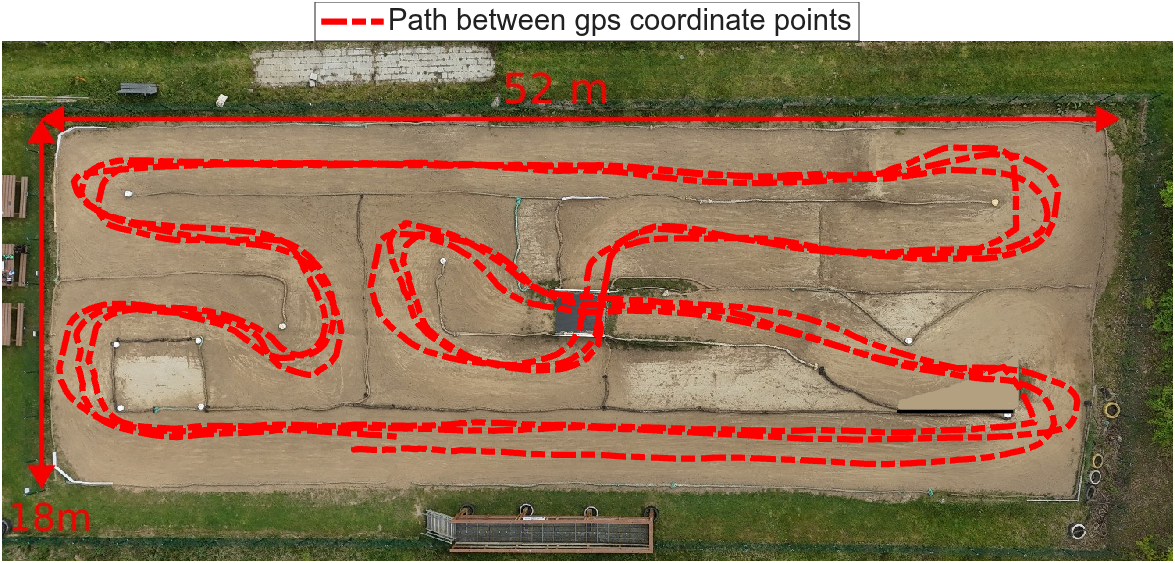
\includegraphics[width=0.5\textwidth]{images/experiments/slow_drive/exp1_fig1.png}
	\caption{
		GPS reference of the TruggySense V2, during the "Slow driving" experiment.
	}
	\label{fig:exp1_fig1}
\end{figure}

\newpage
Fig.~\ref{fig:exp1_fig3_v2} reveals that terrain variations, such as divots, ridges, and slopes, are reflected in the pitch angle: a positive value corresponds to an incline, while a negative value indicates a decline. 
These results are consistent with those of the TruggySense V1 (Fig.~\ref{fig:exp1_fig3_v1}), and further capture track changes, including the displacement of sand from the elevated platform in the bottom-right corner toward the upper lane.

\begin{figure}[!h]
	\centering
    \begin{subfigure}{0.47\textwidth}
        \centering
        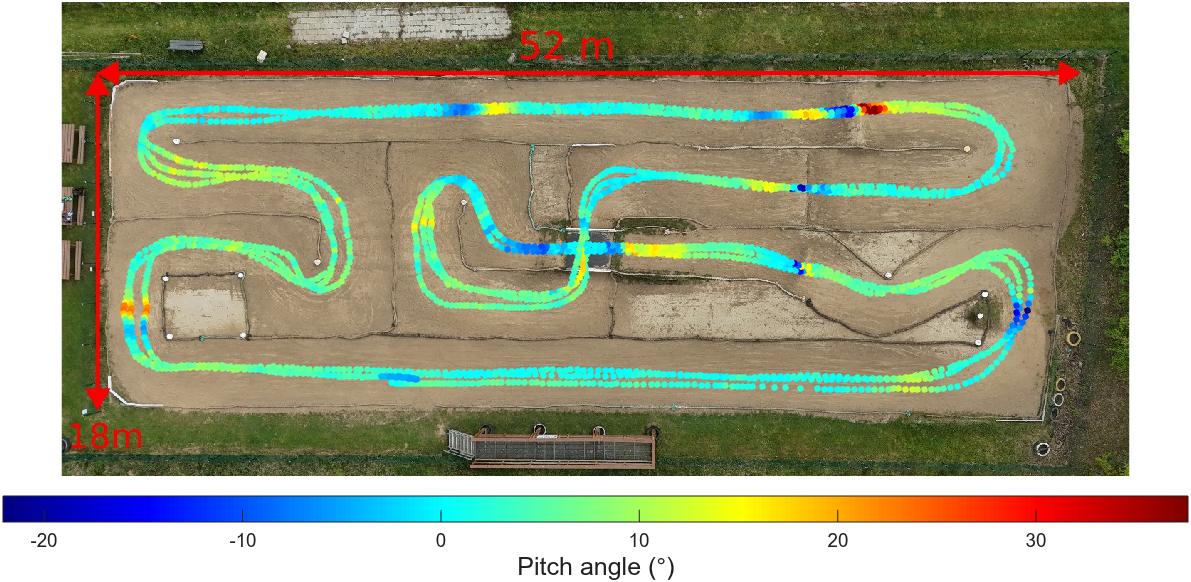
\includegraphics[width=\textwidth]{images/experiments/slow_drive/exp1_fig3_v1.png}
        \caption{Pitch angle of the TruggySense V1.}
		\label{fig:exp1_fig3_v1}
    \end{subfigure}
    \begin{subfigure}{0.47\textwidth}
        \centering
        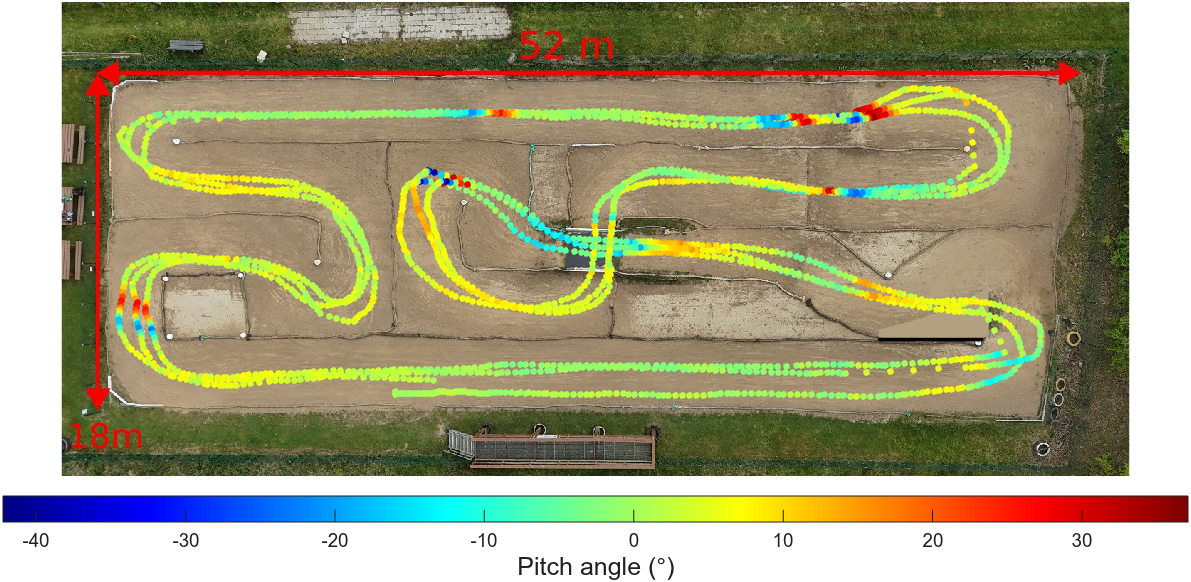
\includegraphics[width=\textwidth]{images/experiments/slow_drive/exp1_fig3_v2.png}
        \caption{Pitch angle of the TruggySense V2.}
		\label{fig:exp1_fig3_v2}
    \end{subfigure}
	\caption{Difference in pitch angle, during the "Slow driving" experiment.}
	\label{fig:exp1_fig3}
\end{figure}

The RCV features three differentials, one at the front, rear, and middle, enabling the wheels to rotate at different speeds whilst turning a corner.
Fig.~\ref{fig:exp1_fig3_v2} demonstrates that the direction of a turn can be discerned from the data gathered by the DAQ: a negative value corresponds to a clockwise turn, while a positive value indicates a counterclockwise turn.
This is consistent with the TruggySense V1 results presented in Fig.~\ref{fig:exp1_fig3_v1}.

\begin{figure}[!h]
	\centering
    \begin{subfigure}{0.47\textwidth}
        \centering
        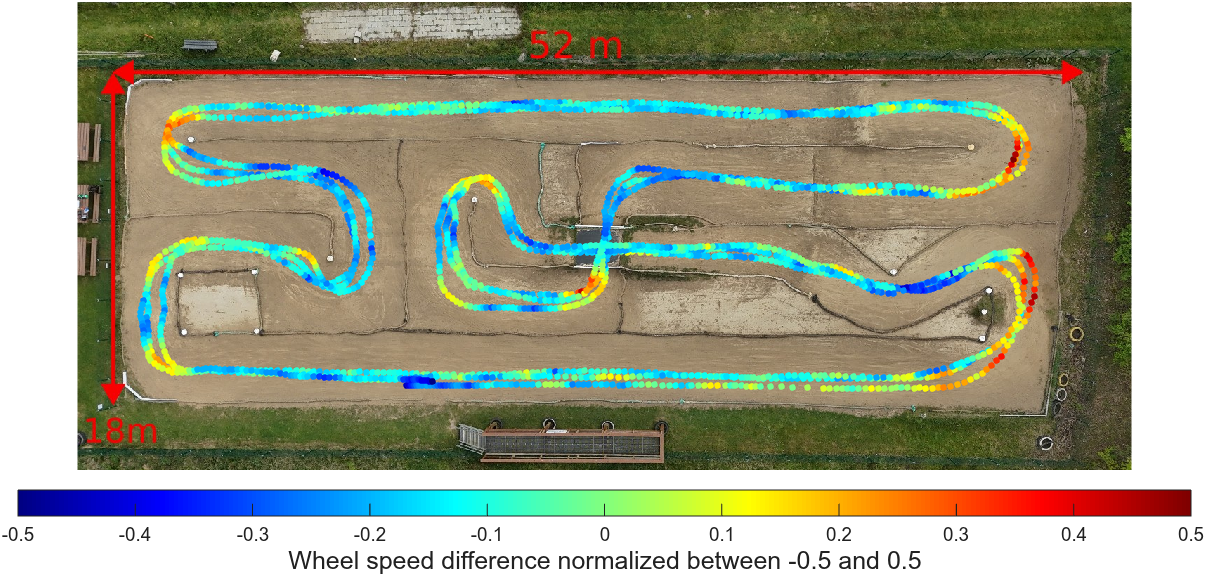
\includegraphics[width=\textwidth]{images/experiments/slow_drive/exp1_fig2_v1.png}
        \caption{Normalized wheel speed difference of the TruggySense V1.}
		\label{fig:exp1_fig2_v1}
    \end{subfigure}
    \begin{subfigure}{0.47\textwidth}
        \centering
        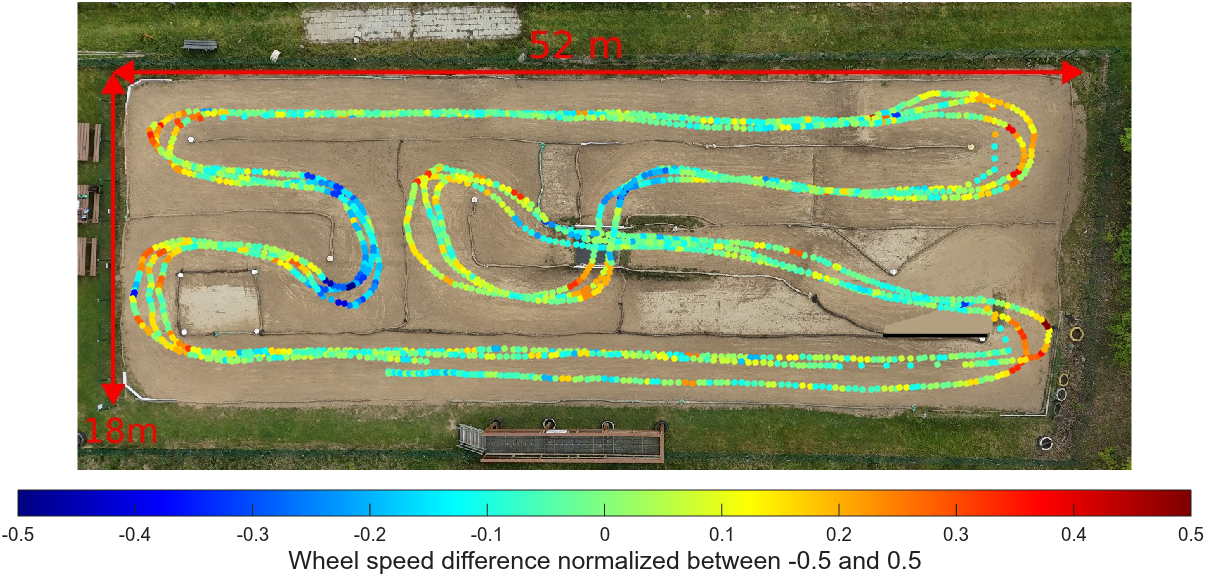
\includegraphics[width=\textwidth]{images/experiments/slow_drive/exp1_fig2_v2.png}
        \caption{Normalized wheel speed difference of the TruggySense V2.}
		\label{fig:exp1_fig2_v2}
    \end{subfigure}
	\caption{Difference in left and right wheel speeds, during the "Slow driving" experiment.}
	\label{fig:exp1_fig2}
\end{figure}


Due to the nature of this experiment, the RCV will have lower power consumption and, in turn, reduced heating.
Fig.~\ref{fig:exp1_fig4} illustrates that the temperatures of the motor ESC $ t_{esc_{1}} $ and $ t_{m_{1}} $ both increased after prolonged usage, while battery pack $ t_{bp} $ and  steering servo $ t_{ss} $ maintained a steady temperature.

\begin{figure}[!h]
	\centering
	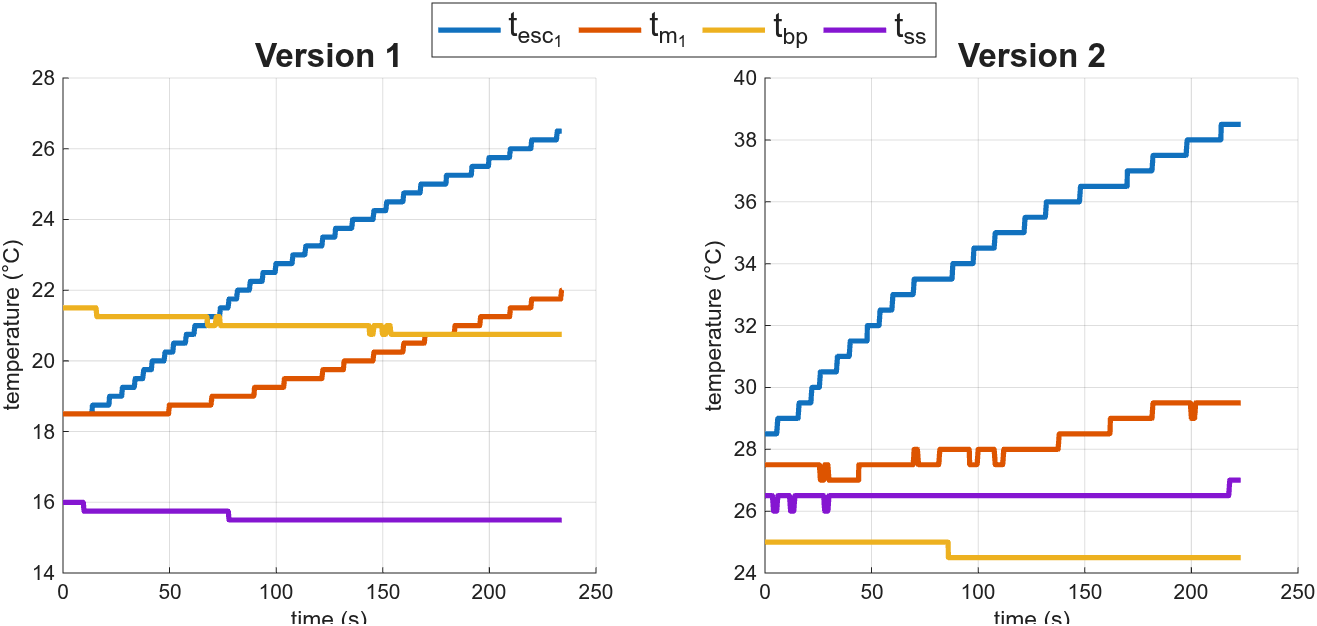
\includegraphics[width=0.5\textwidth]{images/experiments/slow_drive/exp1_fig4.png}
	\caption{
		Temperature comparison of the active components between the TruggySense V1 and V2 during the "Slow driving" experiment.
		The following components where measured: $esc_{1}$ = ESC, $m_{1}$ = Motor, $bp$ = Battery Pack, and $ss$ = Steering Servo.
	}
	\label{fig:exp1_fig4}
\end{figure}

\newpage
\subsubsection{Fast driving over the track}
During this experiment, the RCV was driven at a higher speed than in experiment (1), with a throttle maintained at approximately twice the value used previously.
The increase in speed leads to a wider spacing between the GPS data-points and greater wheel slip, as indicated by the steep inclines and declines in Fig.~\ref{fig:exp2_fig1_v2}.
These results are consistent with those of the TruggySense V1 (Fig.~\ref{fig:exp2_fig1_v2}).

\begin{figure}[!h]
	\centering
    \begin{subfigure}{0.47\textwidth}
        \centering
        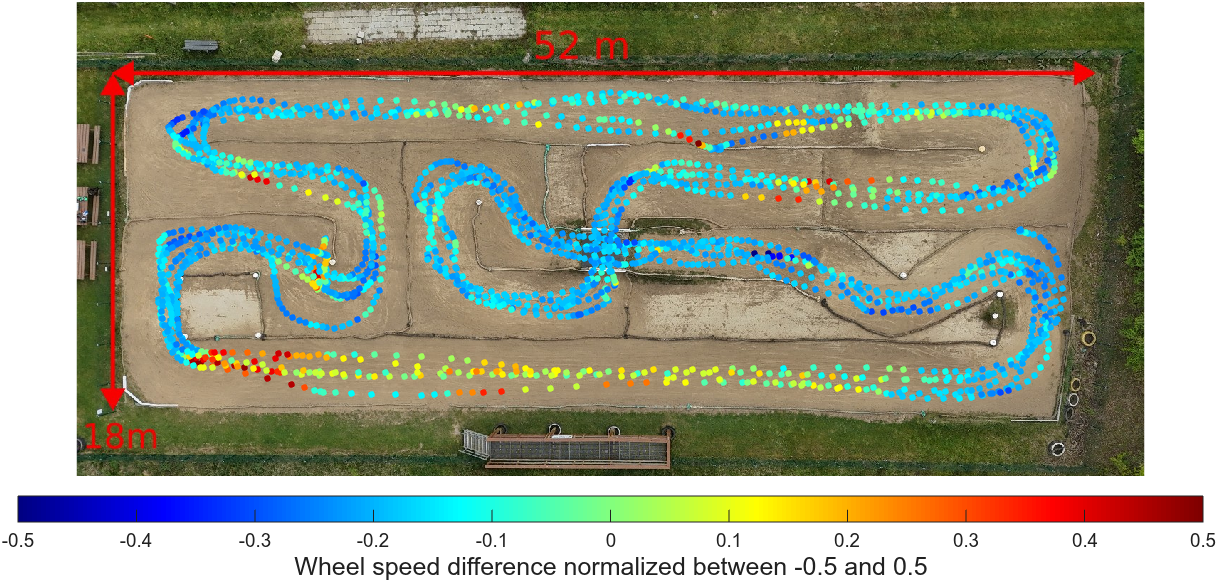
\includegraphics[width=\textwidth]{images/experiments/fast_drive/exp2_fig1_v1.png}
		\label{fig:exp2_fig1_v1}
        \caption{Normalized wheel speed difference of the TruggySense V1.}
    \end{subfigure}
    \begin{subfigure}{0.47\textwidth}
        \centering
        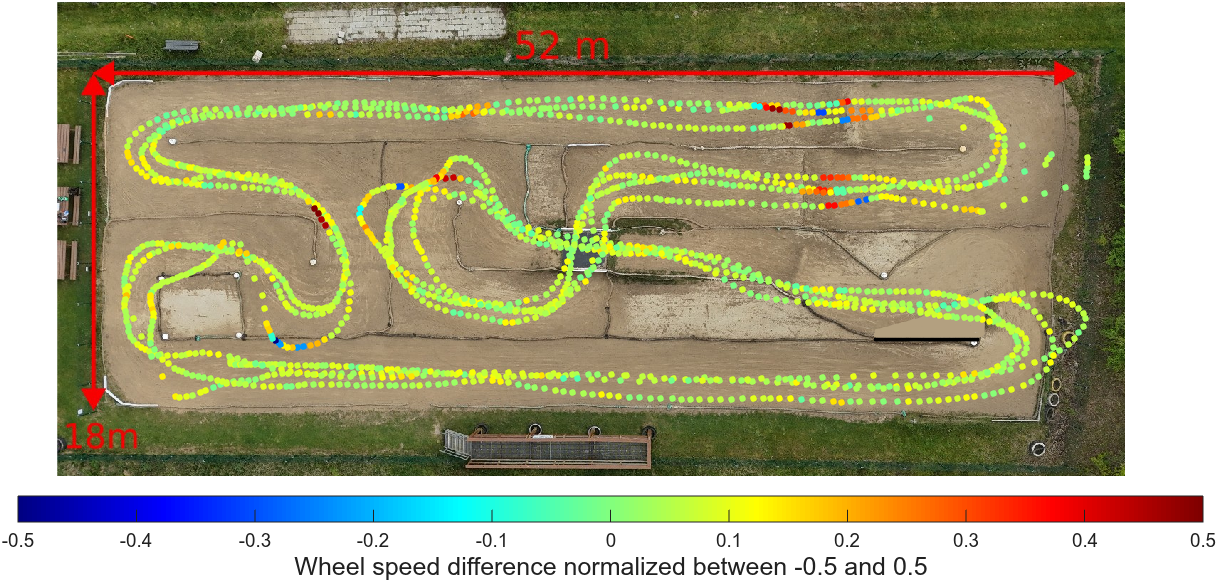
\includegraphics[width=\textwidth]{images/experiments/fast_drive/exp2_fig1_v2.png}
		\label{fig:exp2_fig1_v2}
        \caption{Normalized wheel speed difference of the TruggySense V2.}
    \end{subfigure}
	\caption{Difference in front and back wheel speeds, during the "Fast driving" experiment.}
	\label{fig:exp2_fig1}
\end{figure}

Fig.~\ref{fig:exp2_fig2} compares the temperature difference of the ESC $ t^{f}_{esc_{1}} - t^{s}_{esc_{1}} $, motor $ t^{f}_{m_{1}} - t^{s}_{m_{1}} $ and battery pack $ t^{f}_{bp} - t^{s}_{bp} $, compared to experiment (1).
While there is a temperature increase, it is relatively low compared to the increase that was measured by the TruggySense V1.
This, in combination with the wider distances between GPS data points, suggests that the original tests were done at a higher speed.
Additionally, the change in sensor has introduced a clear reduction in accuracy.

\begin{figure}[!h]
	\centering
	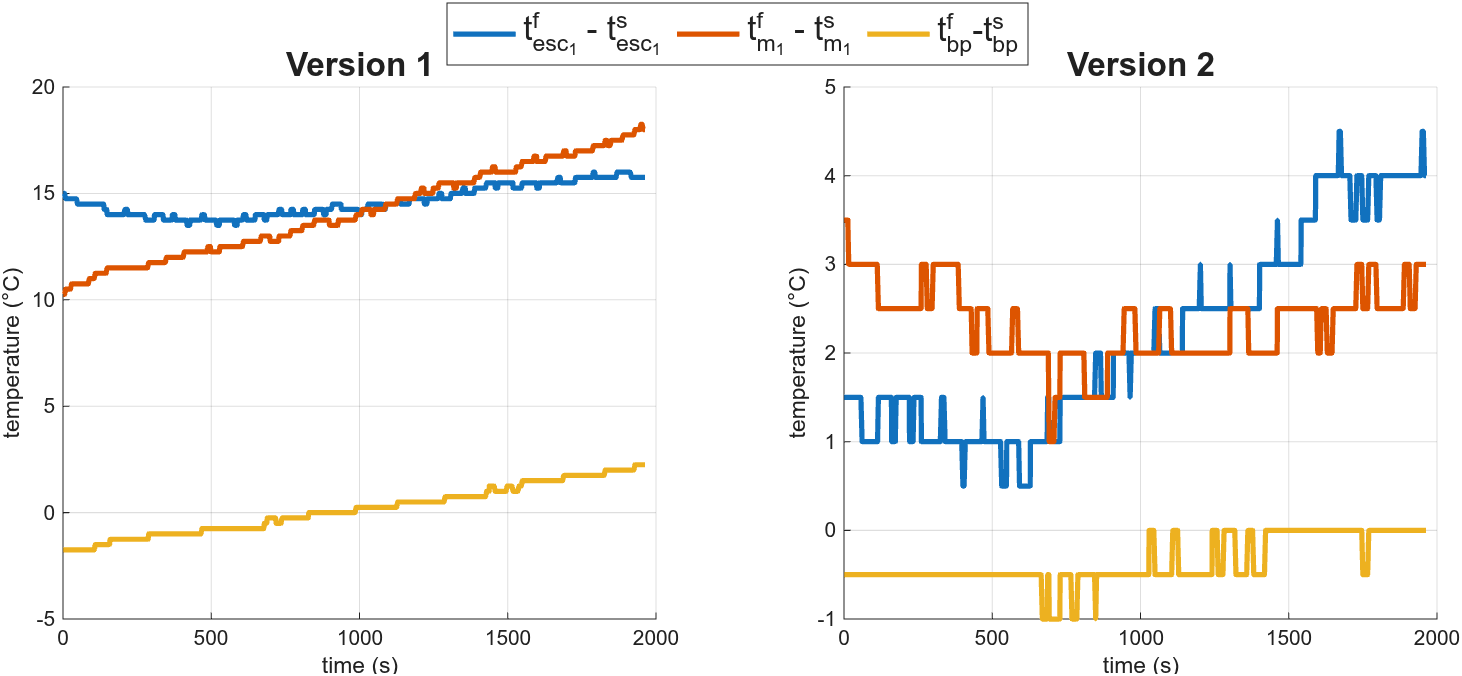
\includegraphics[width=0.5\textwidth]{images/experiments/fast_drive/exp2_fig2.png}
	\caption{
		Temperature difference between "Fast driving" and "Slow driving" experiments of the TruggySense V1 and V2.
		The following components where measured: $esc_{1}$ = ESC, $m_{1}$ = Motor, and $bp$ = Battery Pack.
	}
	\label{fig:exp2_fig2}
\end{figure}

Under higher speeds, minor steering adjustments result in greater turns, which could destabilize the RCV.
However, Fig.~\ref{fig:exp2_fig4} suggests that this affects the TruggySense V2 less than V1.
The cause for this may be due to more precise driver input, a lower operating speed compared to the original "Fast driving" experiment, or the recalibration of the neutral positions of the front wheels to reduce drift\footnote{Unlike the rear wheels, the front wheels are not perpendicular to each other. If they are not calibrated correctly, this could cause the vehicle to drift to one side.}.
Since the difference in speed was already inferred from Fig.~\ref{fig:exp2_fig1} and Fig.~\ref{fig:exp2_fig2}, the lower operating speed is the most likely reason.

\begin{figure}[!h]
	\centering
	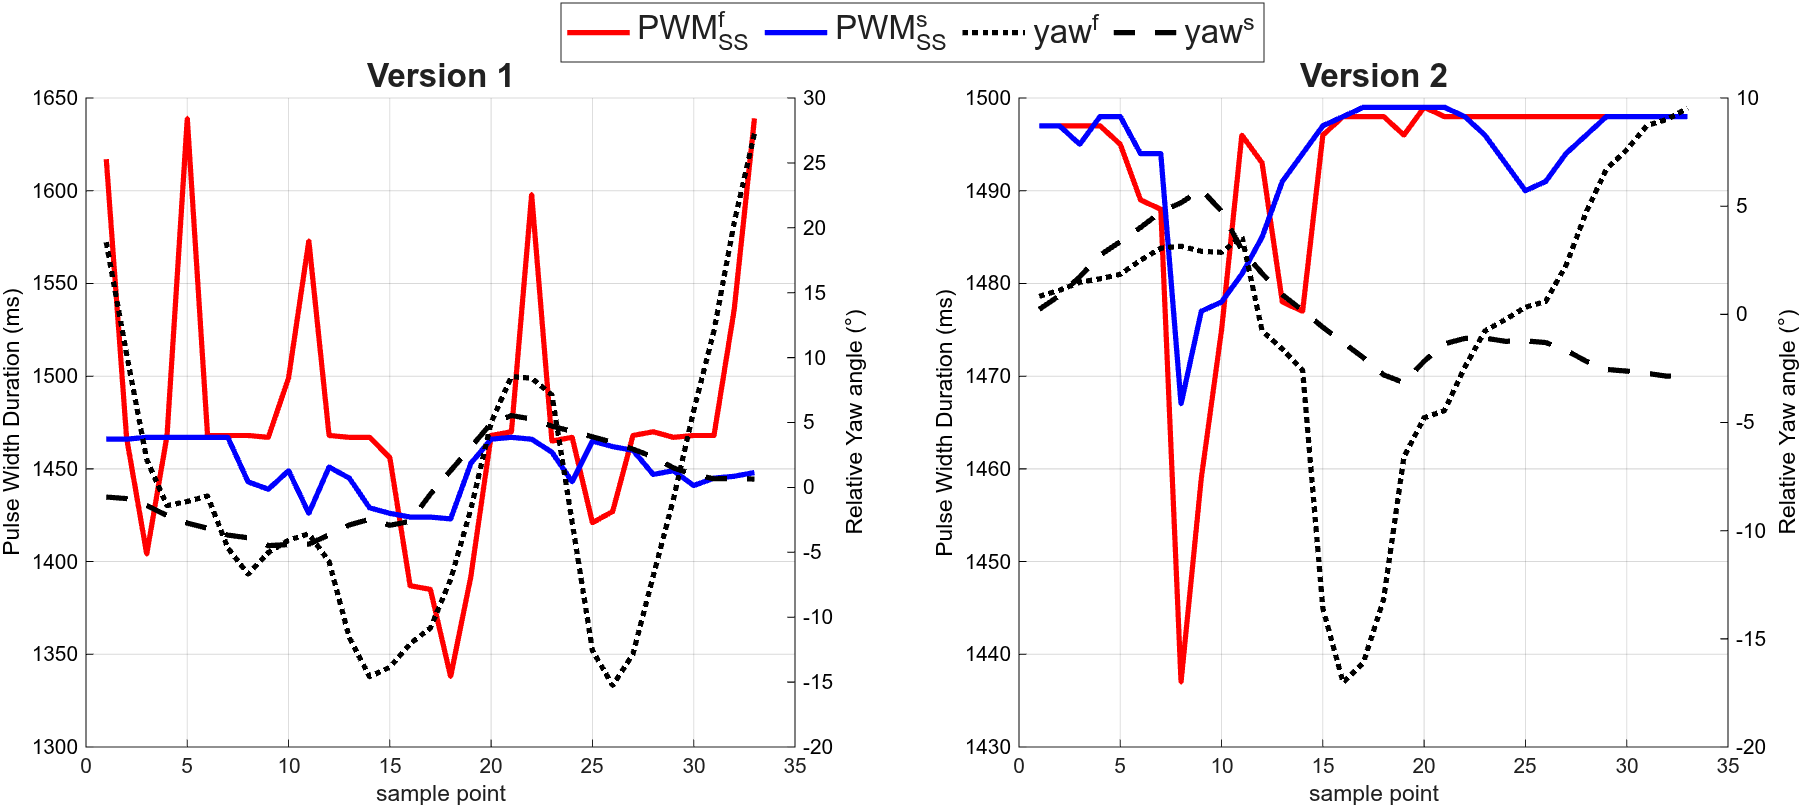
\includegraphics[width=0.5\textwidth]{images/experiments/fast_drive/exp2_fig4.png}
	\caption{
		Raw PWM values of the steering servo with yaw angles between "Fast driving" and "Slow driving" experiments of the TruggySense V1 and V2.
	}
	\label{fig:exp2_fig4}
\end{figure}

\newpage
\subsubsection{Stability and accuracy of the DAQ}
During these experiments, the system was placed upon an elevated platform with the wheels suspended in the air to permit free rotation.
As the majority of the "Slow driving" and "Fast driving" experiments rely on positioning, orientation angles, and wheel speed data, the accuracy of these sensors is evaluated in this section.

Fig.~\ref{fig:exp_position} visualizes the accuracy of the positioning.
Using the Haversine formula~\cite{Robusto1957} --to convert a difference in latitude $\Delta\varphi$ and longitude $\Delta\lambda$ data to meters, compared to the mean radius of the earth $R$-- the distance to the center of each data set can be attained (as presented in Tab.~\ref{tab:position_distance}).
\begin{align}
	a & = \sinsq\left(\frac{\Delta\varphi}{2}\right) + \cos{(\varphi_1)} \cos{(\varphi_2)} \sinsq\left(\frac{\Delta\lambda}{2}\right) \\
	d & = 2 \cdot R \cdot \arctantwo (\sqrt{a},\,\sqrt{1-a})
\end{align}
From this, it can be ascertained that an increase in speed, while driving, does not have a major impact on the accuracy of the GNSS/GPS module, only detecting a 0.15m difference between the "Slow driving" and "Fast driving" experiments.
Noticeably, each data set has shifted results relative to one another, ranging up to 5m.

\begin{figure}[!h]
	\centering
	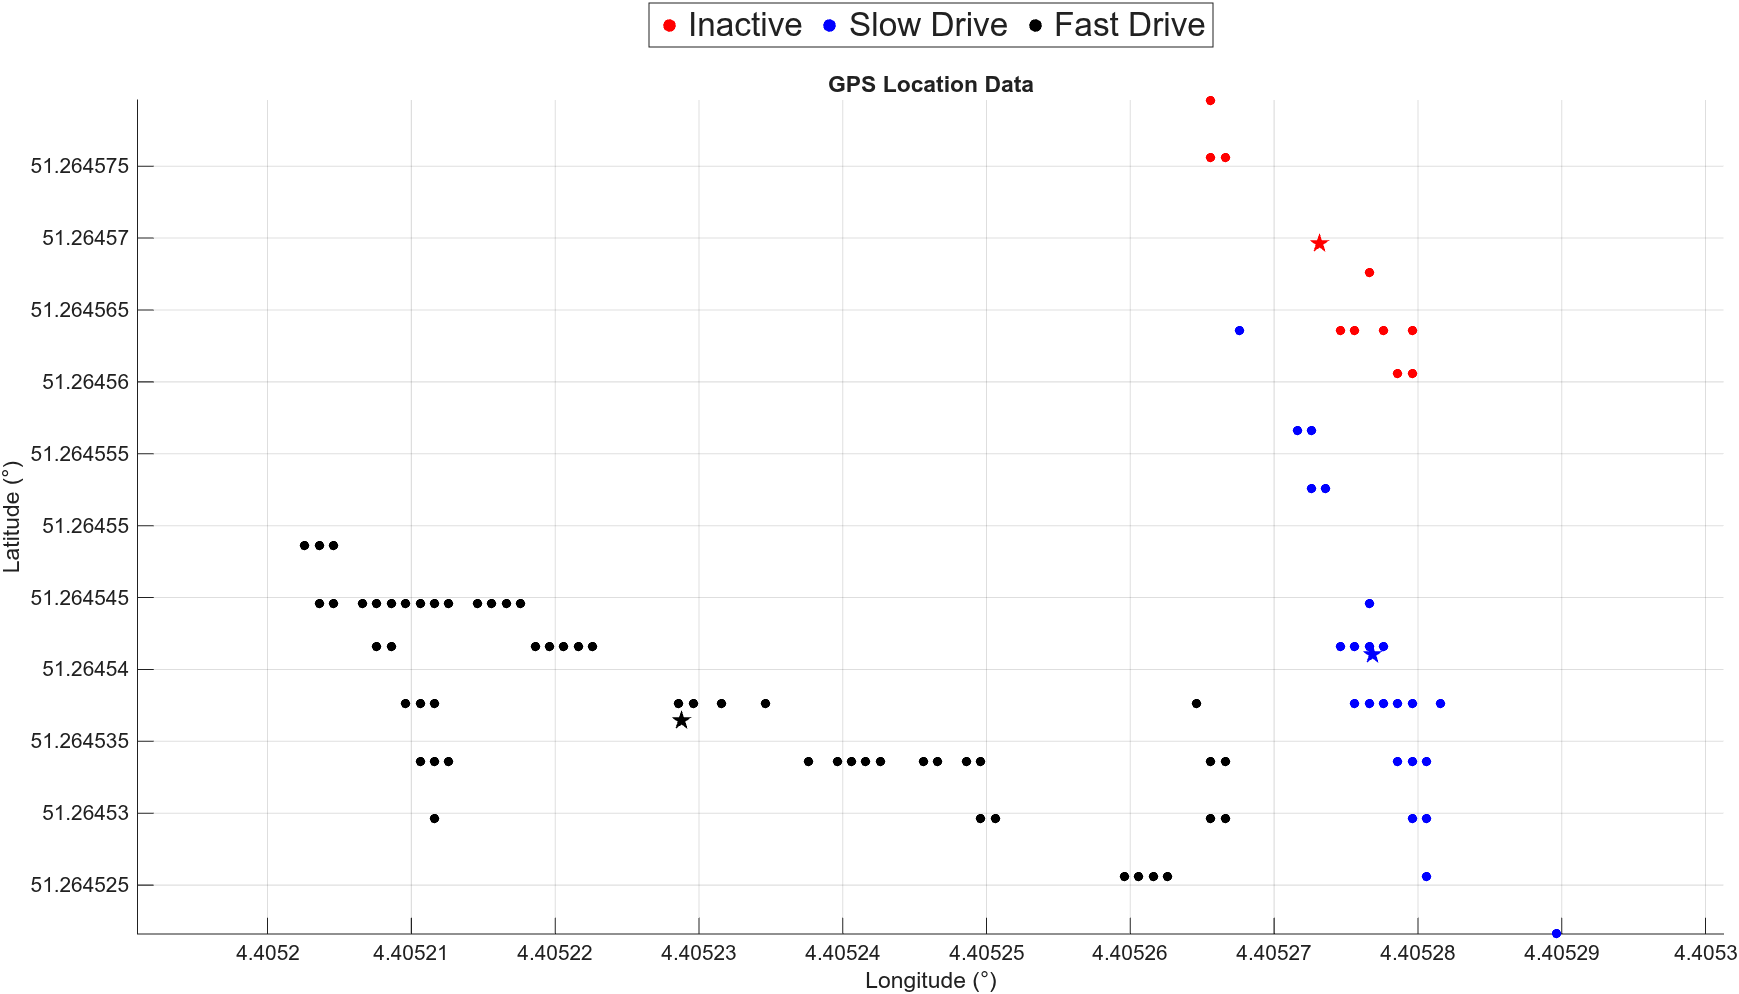
\includegraphics[width=0.5\textwidth]{images/experiments/stationary/exp_position.png}
	\caption{
		The positioning accuracy of the TruggySense V2, while stationary.
		The center point, of each data set, indicated by the pentagram.
	}
	\label{fig:exp_position}
\end{figure}

\begin{table}[!h]
	\centering
	\caption{Positioning deviation}
	\begin{tabular}{lccc}
		\toprule
			Distance to & Standstill (m) & Slow driving (m) & Fast driving (m) \\
		\midrule
			Centroid  & 1.23 & 2.59 & 2.74 \\
			Stationary & 0.00 & 3.19 & 4.81 \\
		\bottomrule
	\end{tabular}
	\label{tab:position_distance}
\end{table}
With, the data in the first row represents the distance from the centroid of each data set, compared to the furthest point in that data set.
And the data in the second row represents the distance of each centroid compared to the centroid of the stationary data set.

Fig.~\ref{fig:exp_wheels} presents the measured rotational speed of each wheel compared to the combined data set.
Across both the "Slow driving" and "Fast driving" experiments, the Front Right (FR) exhibited an above-average rotational speed, while that of the Front Left (FL) was below average.
Implying that, even while suspended, the system steers to the left.

\begin{figure}[!h]
	\centering
	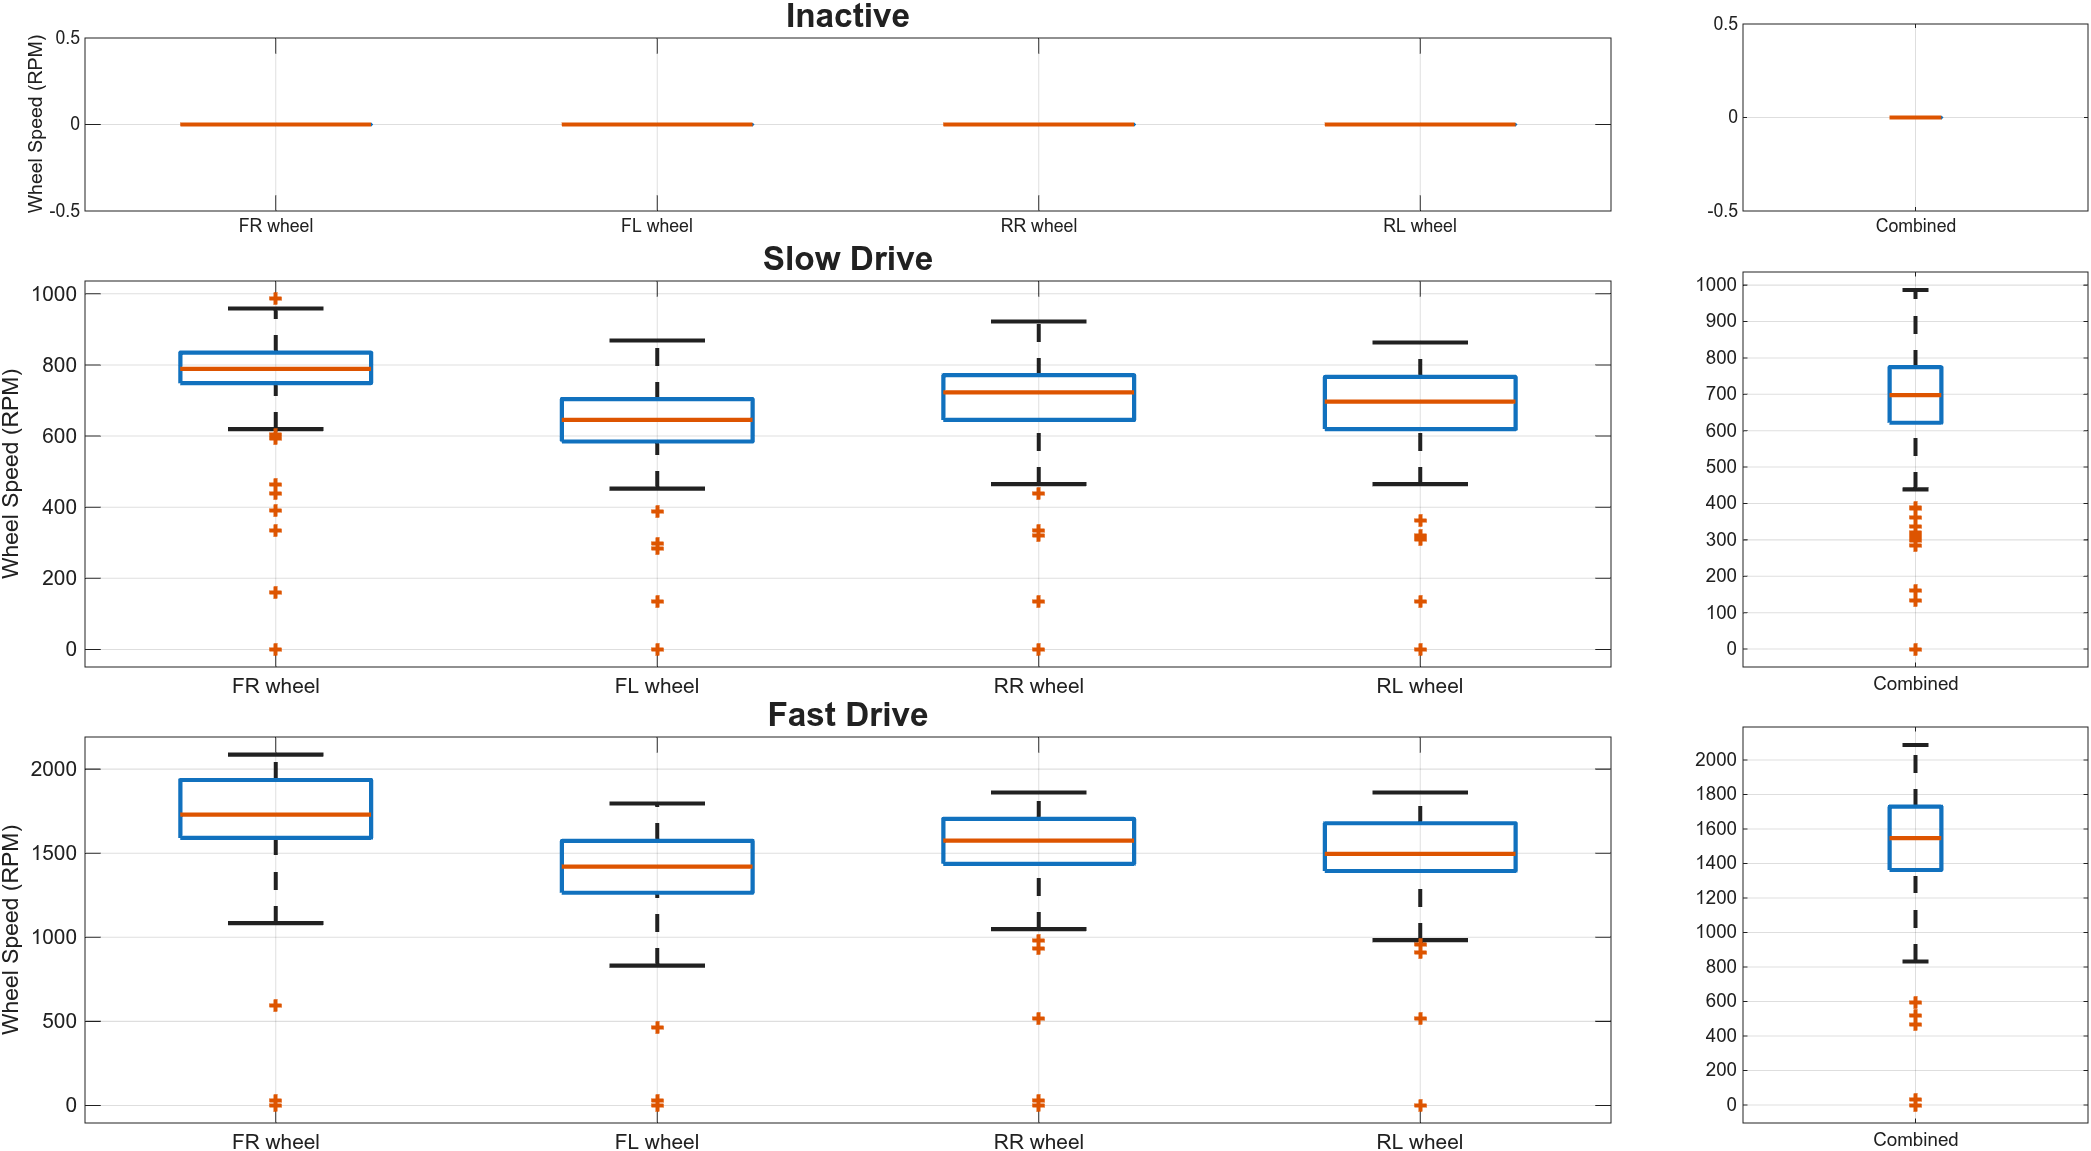
\includegraphics[width=0.5\textwidth]{images/experiments/stationary/exp_wheels.png}
	\caption{Accuracy of the wheel rotation of the TruggySense V2 while stationary.}
	\label{fig:exp_wheels}
\end{figure}

Fig.~\ref{fig:exp_IMU} reveals the stability of the orientation angles.
It clearly reveals that there are disturbances introduced by the rotation of the wheels, and that they increase and become more frequent with an increase in rotational speed.
Nevertheless, even for the "Fast drive" experiment, these deviations remain within approximately $\pm$1° across all orientation angles.
This suggests that the placement of the IMU has no effect on its operational capabilities, and thus can be mounted to the PCB instead of the bottom plate of the chassis.

\begin{figure}[!h]
	\centering
	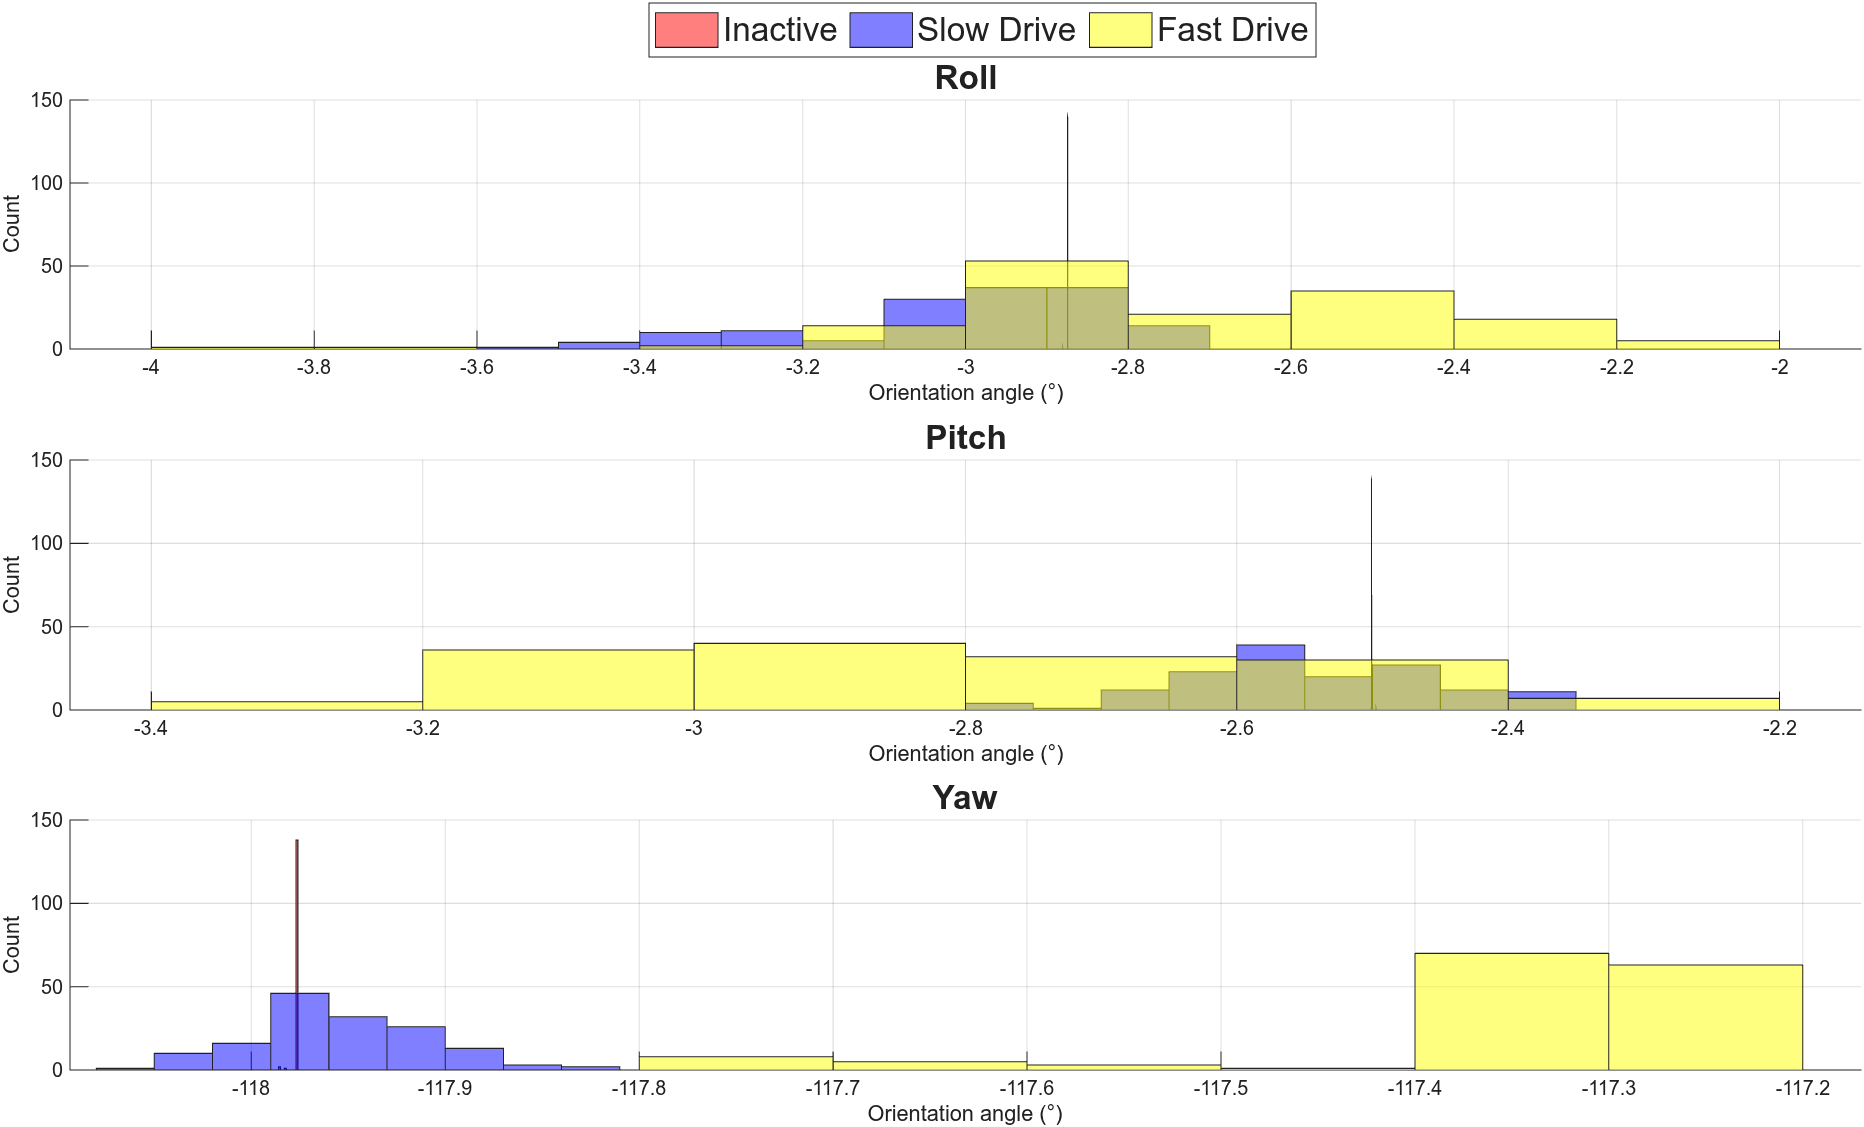
\includegraphics[width=0.5\textwidth]{images/experiments/stationary/exp_IMU.png}
	\caption{Accuracy of the orientation angles of the TruggySense V2 while stationary.}
	\label{fig:exp_IMU}
\end{figure}

\newpage
\section{Discussion and Conclusion}
This project presents the modifications made to the TruggySense V1 and evaluates their impact on the DAQ system. 
It confirms that the system remains capable of ascertaining real-world behavior and key metrics, including driving speed, wheel slip, and orientation, while retaining its accuracy.
Furthermore, it introduces support for IWD and system expansion, while simplifying the hardware assembly.
On top of that, it reduces the overall complexity of the system, streamlining the integration of new modules in both hardware and firmware.

However, several limitations still remain. 
It is still unclear whether the system supports reverse polarity protection, and while support for redundancy has been added, full redundancy has not been implemented. 
Additionally, another attempt at integrating ROS2 was made, but did not yield any discernible progress.
Beyond that, the losses introduced by the new temperature sensors do not justify the replacement of the old ones.

This work continued on the solid foundation that was provided by the TruggySense V1, making it more approachable for the student who will continue to work on it.
Just like its predecessor, it did not focus on groundbreaking scientific discoveries but continued to build a foundation that has the potential to make an impact within the context of engineering education.
One enhancement that could be introduced is the addition of both RADAR and LiDAR technology.
This, in turn, would lay the groundwork for turning this RCV system into a fully autonomous vehicle, capable of comprehending and navigating any off-road environment.

\chapter{Contacts}                  % ---------------------- Contacts ----------------------

\section{Student}
\begin{itemize}
    \item Thomas Kramp
    \item +32 471 48 29 13
    \item thomas.kramp@student.uantwerpen.be
\end{itemize}

\section{Internal Supervisor}
\begin{itemize}
    \item Jan Steckel
    \item +32 3 265 2312
    \item +32 497 86 38 95
    \item jan.steckem@uantwerpen.be
\end{itemize}

\section{Hardware consultants}
\begin{itemize}
    \item Dennis Laurijssen
    \item +32 3 265 16 95
    \item dennis.laurijssen@uantwerpen.be
\end{itemize}
\begin{itemize}
    \item Eric Paillet
    \item eric.paillet@uantwerpen.be
\end{itemize}
\begin{itemize}
    \item Simon Sleutel
    \item simon.sleutel@uantwerpen.be
\end{itemize}

\chapter*{AI Usage}
\begin{table}[h!]
    \centering
    \begin{tabular}{ll}
        \toprule
            \textbf{LLM} & \textbf{Used for} \\
        \midrule
            ChatGPT     & Use of this model has been added in the "docs/ai\_use/directory/chatgpt". \\
            Claude      & Use of this model has been added in the "docs/ai\_use/directory/claude". \\
            Copilot     & Used for the documentation inside the codebase, such as the "@brief"-notes. \\
            Grammerly   & Used to find and fix spelling errors. \\
        \bottomrule
    \end{tabular}
\end{table}

% References Section

\chapter*{Bibliography}

% The following lines set up the bibliography using BibTeX
\bibliographystyle{IEEEtran}
\bibliography{bibliography} % Replace 'bibliography' with the name of your .bib file


% \makefinalpage
\end{document}